\documentclass[12pt]{article}
%\usepackage[showframe]{geometry}% http://ctan.org/pkg/geometry
\usepackage{lipsum}% http://ctan.org/pkg/lipsum
\usepackage{multicol}% http://ctan.org/pkg/multicols
\usepackage{graphicx}% http://ctan.org/pkg/graphicx
\usepackage{float}
\usepackage{fancyhdr}
\usepackage{titling}
\usepackage{subcaption}
\usepackage{indentfirst}
\usepackage{booktabs}
\usepackage{multirow} 
\usepackage{setspace} \doublespacing
\usepackage{mathptmx}
\usepackage{amsmath}
\usepackage[backend=biber, style=apa,]{biblatex}
\usepackage{hyperref}
\usepackage{float}
\usepackage{caption}
\usepackage{sectsty}
\usepackage{titlesec} % Add titlesec package

\pagestyle{fancy}
\doublespacing

%\addbibresource{/mnt/c/Users/woute/projects/Thesis_endstop/MyLibrary.bib}
% \addbibresource{/home/wouter/projects/Thesis_endstop/latex_endstop/MyLibrary.bib}
\addbibresource{MyLibrary.bib}

\hyphenpenalty=1000
\tolerance=2000

\fancyhead{}
\fancyfoot{}
\fancyfoot[R]{\thepage}
\renewcommand{\headrulewidth}{0pt}

% Adjust header whitespace
\setlength{\headheight}{5pt}  % Adjust as needed
\setlength{\headsep}{5pt}     % Adjust as needed

\setlength{\droptitle}{-10em}   % This is your set screw
\setlength{\parindent}{0pt}

\sectionfont{\large} % Change \Large to your desired size
%\subsectionfont{\normalsize} % Change \large to your desired size

% Center the section titles
\titleformat{\section}
  {\normalfont\Large\bfseries\filcenter} % Format: font size, weight, alignment
  {\thesection}{1em}{} % Label and separation from title

\begin{document}

\captionsetup{font=small}

\begin{titlepage}
\centering

% Adjust font size and family as needed
{\LARGE\bfseries Hierarchical Circuit Structure of Mouse Visual Cortex for Generating Illusory Contour Responses\par}

% \vspace{2pt} % Adjust space between title and figure as needed

% Include the figure

\includegraphics[width=0.5\textwidth]{figures/donders_logo.png}

\includegraphics[width=0.5\textwidth]{figures/uva_logo.png}
\begin{center}
  MSc Biomedical Sciences:\\
  Cognitive Neurobiology and Clinical Neurophysiology
\end{center}

\vspace{10pt} % Adjust space between figure and author/date as needed

% Author and Date
{\large Wouter Kroot\par}
\vspace{5pt} % Adjust as needed
{\large April 2024\par}
\vspace{5pt}
{\large Supervisor: Prof. dr. P.H.E. Tiesinga}

\end{titlepage}

% Rest of the document starts here
\newpage

% Abstract
\vspace*{-\headsep}
\vspace*{-\headheight}
\vspace*{-60pt} % Adjust the value to move the figure up
\begin{abstract}
  \small
  \frenchspacing
  % Recent studies of the mouse visual system demonstrated their ability to perceive illusory contours and identified feedback responses to be crucial for the illusory activity measured in the primary visual cortex (V1). Complementing these findings, computational work has shown that length-tuned endstopped cells are capable of delineating visual boundaries between objects, particularly when objects are ambiguous or occluded. Motivated by these findings, we aimed to simulate illusory contour processing to further discern the contribution of recurrent activity to illusory contour responses in V1. We developed a Leaky Integrate and Fire based model, along with population firing rate models, to identify the requirements needed for stable endstopping and to demonstrate how the integration of endstopped cells facilitate the representation of illusory contours. Our findings indicate that orientation-selective and length-tuned endstopped cells are a suitable neural mechanism for detecting the line ends that induce the abutting grating illusion. Furthermore, we demonstrate that recurrent inhibition enables a gradual decrease in endstopping behaviour for stimulus configurations that deviate from an endstopped cell's preferred input. By replicating endstopped responses in a population rate-based model, we show how hierarchical interactions between V1 and higher visual areas integrate endstopped cues to create perceptual boundaries matching illusory contours. These boundaries are amplified and filled in by excitatory recurrent feedback, lifting the illusory figure from the collective organisation of inducers. Our findings demonstrate how the cortex can supply missing information through recurrent connections, while also highlighting the potential of using mice as effective models to explore cortical architectures comparable to those in primates, providing broader implications for understanding cortical organisation across species.

  Illusory contours are edges that are perceived while no physical boundary is present. Recent studies demonstrated that mice can perceive illusory contours and identified feedback responses to be crucial for the illusory-induced activity measured in the primary visual cortex (V1). Additionally, computational work has shown that length-tuned endstopped cells can be used to delineate visual boundaries between objects, particularly when objects are partly occluded. Motivated by these findings, we propose two complementary models capable of representing the abutting grating illusion with a realistic hierarchical organisation of the mouse visual system. The first model is a Leaky Integrate and Fire (LIF) based model used to identify the requirements needed for stable endstopping. Results from the LIF model shows that when endstopped end zones are modulated by indirect inhibitory feedback mechanisms, stability is maintained when input deviates from the cell's preferred orientation. The second model, a population firing rate-based model, replicated the endstopping behaviour from the LIF model and demonstrated how hierarchical interactions between V1 and higher visual areas can integrate endstopped cues to create perceptual boundaries that match illusory contours. These boundaries are amplified and filled in by excitatory recurrent feedback connection to V1, lifting the illusory figure from the collective organisation of inducers. Our models demonstrate how the visual cortex can fill in missing information through recurrent connectivity while also highlighting the potential of using mouse models to explore cortical organisation comparable to those in primates.
  \bigbreak
  \textit{Keywords:} Illusory contours, Endstopped cells, Primary visual cortex, recurrent activity
\end{abstract}


% \newpage
% {\scriptsize
% \tableofcontents}

\newpage

\section*{Introduction}
The mammalian visual system is a complex network of interconnected areas that together process external inputs. Information enters the visual system as two-dimensional retinal activation patterns that are transformed into a coherent three-dimensional representation in the cortex. An essential part of this process is the ability to segment visual scenes into objects distinct from their background and other objects \autocite{kirchbergerEssentialRoleFeedback2020}. Early visual areas, such as the primary visual cortex (V1), perform a local analysis of visual features within relatively small receptive fields and feed their output to higher visual areas (HVAs) that integrate that information over a larger spatial extent and process increasingly abstract features. Some simple features consist of contrast and orientation, more abstract features can be shapes and ultimately encode object category \autocite{ashbridgeEffectImageOrientation2000}. Visual input in V1 is often clearly defined, e.g., by a luminance contrast that indicates a discontinuity such as an edge or a corner. In other cases, feedforward information can be unclear and require further processing for a robust global representation. For example, when an object is occluded by another object, the visual system must make perceptual inferences about the occluded figure and has to fill in the missing details. Interestingly, specific stimulus arrangements can induce the perception of an occluding object while no physical contour is present. Such figures are also known as illusory contours. Because the perception of illusory contours are a direct product of the underlying neural circuitry, they can effectively be used to investigate the neurophysiological interactions required to make inferences about ambiguous or incomplete visual information.
\bigbreak
Although many stimulus configurations make it possible to induce the perception of illusory contours, they often share common features \autocite{palmerLateInfluencesPerceptual2000}. Consider the abutting grating illusion \autocite{sorianoAbuttingGratingIllusion1996} and the Kanizsa triangle illusion \autocite{kanizsaSubjectiveContours1976}. Both illusions involve extrapolations from visual cues that suggest the presence of an occluding object. In the Kanizsa square illusion, three pacman-shaped figures are arranged such that a continuous contour seems to connect the edges of the inducers. Thereby creating the illusion of a square overlapping four circles \hyperref[fig:figure_1]{(figure 1a)}. Similarly, in the abutting grating illusion, the vertical alignment of horizontal lines creates the impression of a vertical contour superimposed on horizontal inducers \hyperref[fig:figure_1]{(figure 1 b)}. In both illusions, inducer input consists of seemingly simple geometrical forms, however, for the resulting illusion to emerge from the background inducers, they require sophisticated processing of individual inducer shapes. Namely, their position and orientation need to be processed in relation to each other. This inter-object complexity necessitates the integration of segmented stimuli, involving either hierarchical feedforward convergence or the local integration of feedback activity. 

\begin{figure}[H]
  \centering
  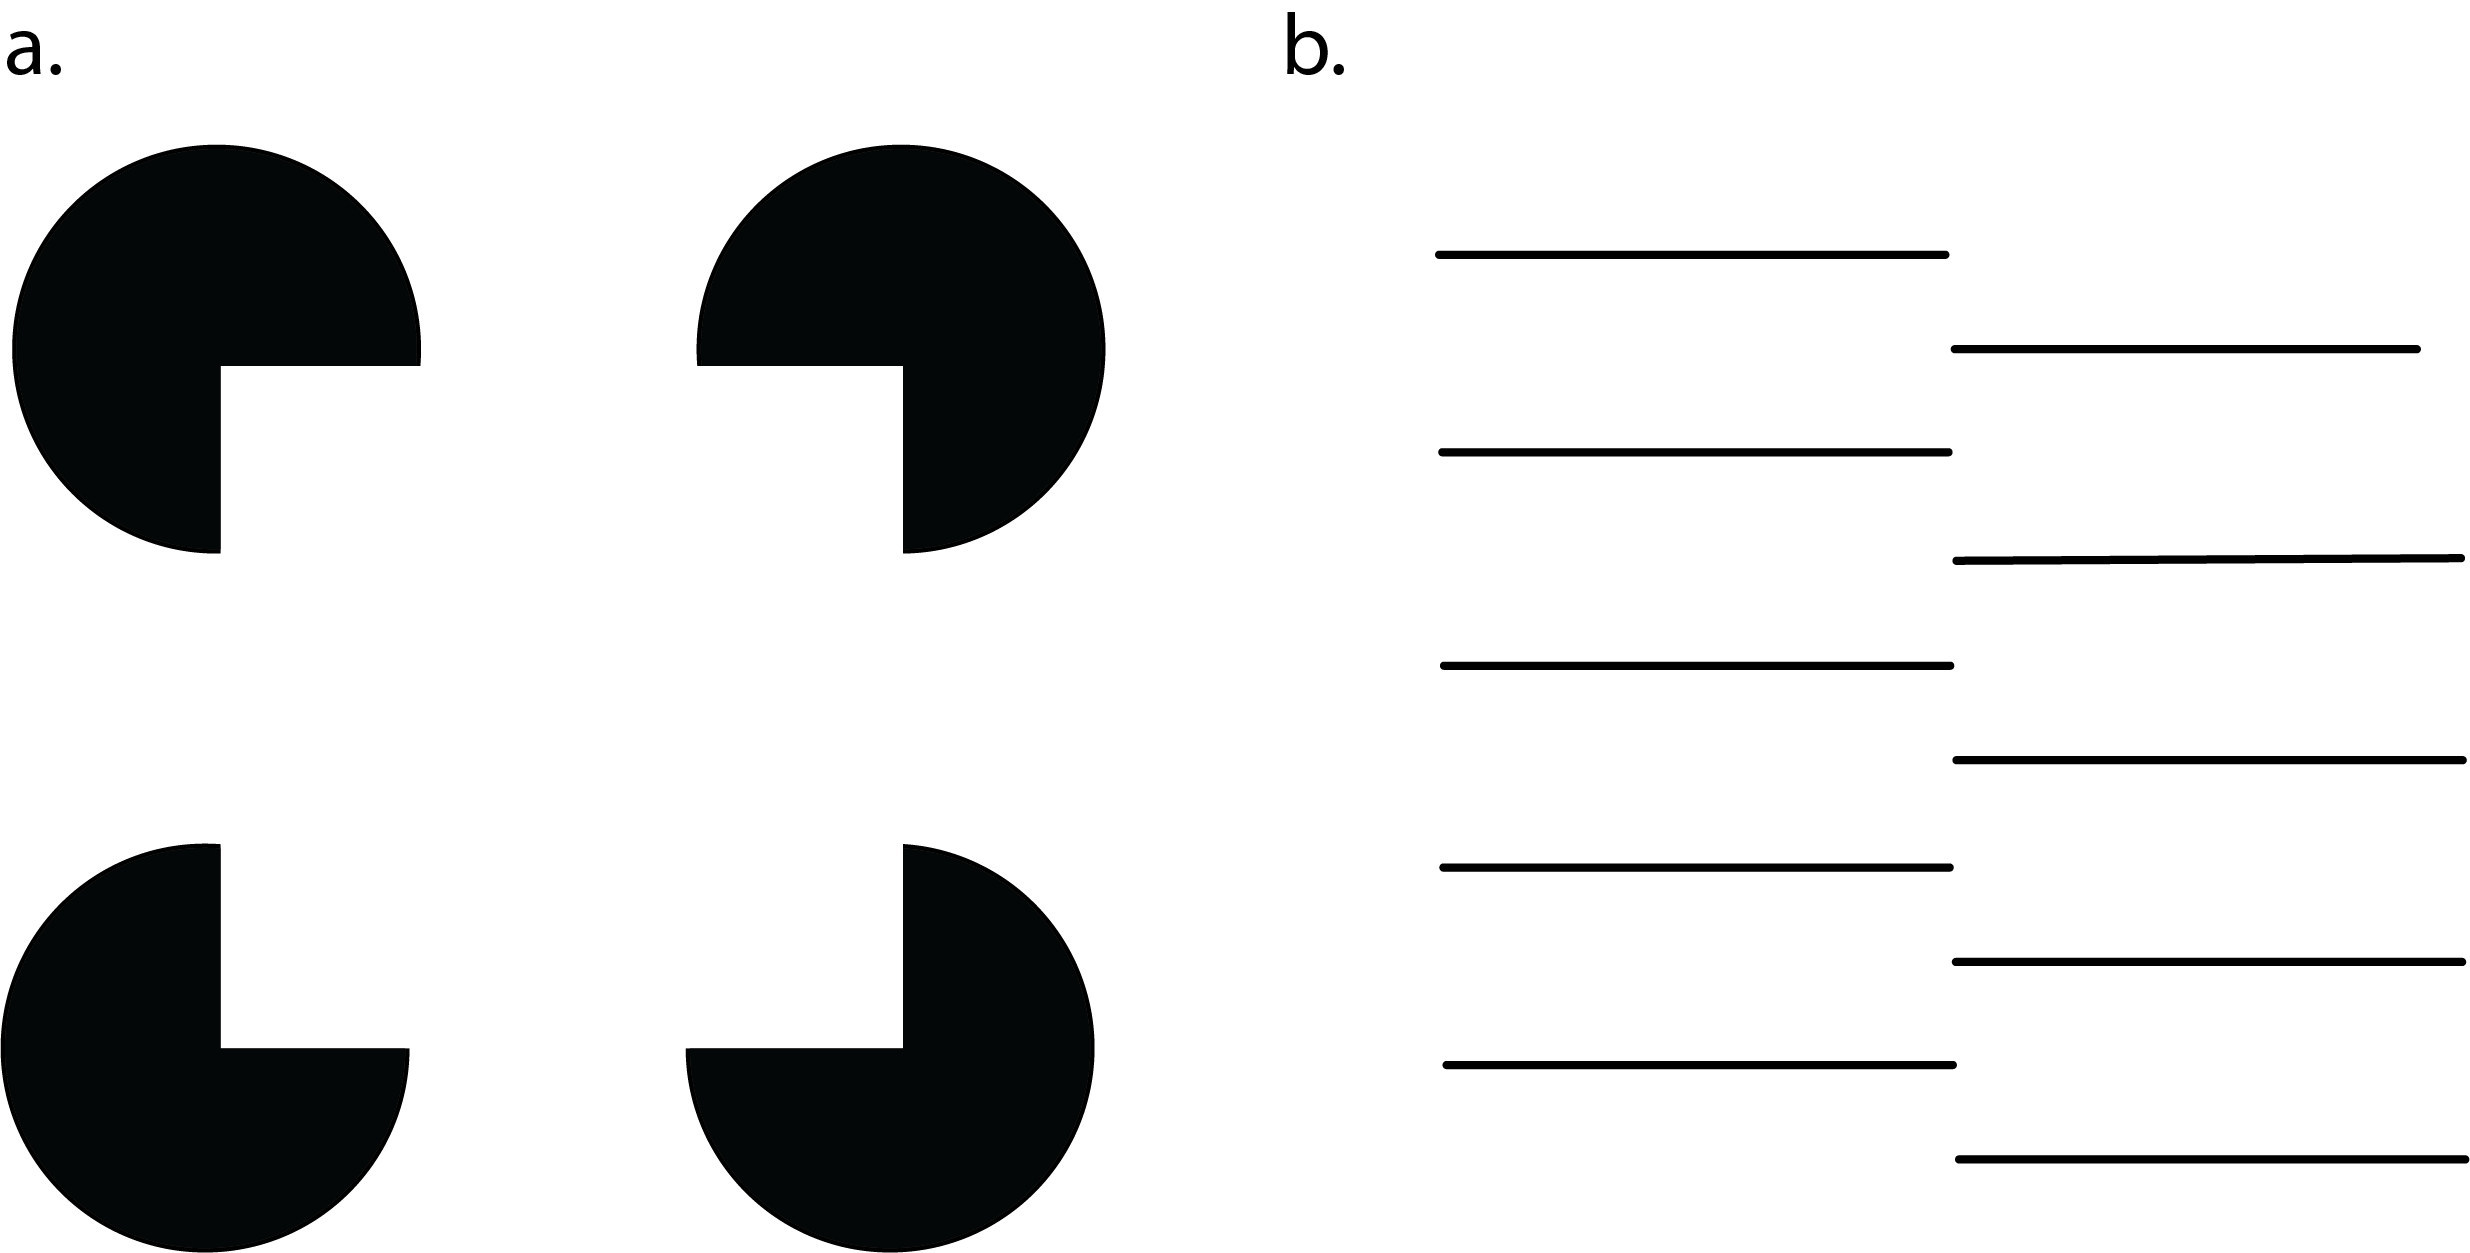
\includegraphics[width=1.0\textwidth]{adjusted_figures/illusory_figures_kanizsa_grating.png}
  \caption{Illusory contour inducing figures. a. The Kanizsa illusion \autocite{kanizsaSubjectiveContours1976}. Four pac-man shaped inducers can be perceived as four circles with an overlapping white square. b. The Abutting grating illusion \autocite{sorianoAbuttingGratingIllusion1996}. The alignment between the horizontal inducers gives the impression of a vertical contour in between the horizontal lines.}
  \label{fig:figure_1}
\end{figure}

% Single-unit recordings from primates have identified neurons in V1 and secondary visual area V2 (~30\% of cells) that react to illusory contours \autocite{vonderheydtMechanismsContourPerception1989}. Interestingly, the response times in V2 precede those in V1, indicating that the first place sensitive for illusory contours in the rhesus macaque is in V2 \autocite{leeDynamicsSubjectiveContour2001}. A possible reason for this delay is that top-down feedback from V2 might supply the missing information about illusory contours to V1. Moreover, recurrent processing is involved in the perception of various illusions, suggesting that interactions between V1 and higher-order processing may be important for the generation of illusory perception \autocite{deweerdCuedependentDeficitsGrating1996,mendolaRepresentationIllusoryReal1999,panEquivalentRepresentationReal2012}. Recurrent activity, which includes both horizontal and their induced feedback connections are demonstrated to play an important role during visual organisation \autocite{roelfsemaCORTICALALGORITHMSPERCEPTUAL2006}. This type of activity helps to integrate local and global visual features, aiding in the grouping of behaviourally relevant objects and their separation from the background. By iteratively refining visual representations, recurrent processing can effectively enhance the perception of complex visual scenes \autocite{roelfsemaCORTICALALGORITHMSPERCEPTUAL2006,shushruthStrongRecurrentNetworks2012}. This recirculation of information is associated with synaptic and conduction delays and would fit the 55 ms delay observed during the filling in process of illusory contours \autocite{leeDynamicsSubjectiveContour2001,pakTopDownFeedbackControls2020}. From this perspective, illusory contours may result from a recurrent process that fills in contour information between specific inducing points that relayed within the feedforward visual input, creating the global perception of a superimposed object. If V2 illusory responses are a product of recurrent activity and real and illusory contours are processed by the same cells, a direct implication would be that higher visual areas might be unable to distinguish between real and illusory contours.
Single-unit recordings from primates have identified neurons in V1 and secondary visual area V2 (\textasciitilde30\% of cells) that react to illusory contours \autocite{vonderheydtMechanismsContourPerception1989}. Interestingly, the response times in V2 precede those in V1, indicating that the first place sensitive for illusory contours in the rhesus macaque is in V2 \autocite{leeDynamicsSubjectiveContour2001}. A possible reason for this delay is that top-down feedback from V2 might supply the missing information about illusory contours to V1. Moreover, recurrent processing, which includes both horizontal and induced feedback connections, is involved in the perception of various illusions, suggesting that interactions between V1 and higher-order processing may be important for the generation of illusory perception \autocite{deweerdCuedependentDeficitsGrating1996,mendolaRepresentationIllusoryReal1999,panEquivalentRepresentationReal2012,roelfsemaCORTICALALGORITHMSPERCEPTUAL2006}.

Recurrent activity, which includes horizontal and induced feedback connections, helps to integrate local and global visual features. This process aids in the grouping of behaviourally relevant objects and their separation from the background. By iteratively refining visual representations, recurrent processing can effectively enhance the perception of complex visual scenes \autocite{roelfsemaCORTICALALGORITHMSPERCEPTUAL2006,shushruthStrongRecurrentNetworks2012}. This recirculation of information is associated with synaptic and conduction delays and would fit the 55 ms delay observed during the filling in process of illusory contours \autocite{leeDynamicsSubjectiveContour2001,pakTopDownFeedbackControls2020}. From this perspective, illusory contours may result from a recurrent process that fills in contour information between specific inducing points that are relayed within the feedforward visual input, creating the global perception of a superimposed object. In the case that V2 illusory responses are a product of recurrent activity and real and illusory contours are processed by the same cells, a direct implication would be that higher visual areas might be unable to distinguish between real and illusory contours.

\bigbreak
This hypothesis has been examined, identifying area V4 in macaques as a crucial integration point where both real and illusory contours are represented equivalently \autocite{panEquivalentRepresentationReal2012}. Through the use of optical imaging and single-cell recordings to compare neural activity elicited by real and illusory contours across areas V1, V2, and V4, it was found that activities in V1 and V2 predominantly relate to the encoding of local spatial features of the inducers, rather than the global orientation of the illusory contour. Meanwhile, V4 processes both real and illusory contours similarly, suggesting that hierarchical interactions govern the global orientation processing of illusory contours. 

Further support for the vital role of recurrent processing in the generation of illusory contours is provided by studies performed in mice. Because the extensive genetic toolkit available for mice that allows for the precise recording and stimulation of specific cells, they are exceptionally well-suited for investigating the hierarchical processing that underpins illusory contours. Akin to the neural delays found in the macaque, mice exhibited a 30 ms delay in the representation of illusory contours compared to contours from real contrast \autocite{pakTopDownFeedbackControls2020}. They trained mice to differentiate between stimuli with and without illusory contours, linking their behaviour to neural activity. They showed that the representation of illusory contours in V1 was eliminated upon the silencing of LM through optogenetics, which aligns with the idea that feedback provides V1 with illusory induced activity \autocite{wyatteEarlyRecurrentFeedback2014}. Although, these findings do not directly show that the generation of illusory contours is dependent on recurrent connectivity they do highlight the role of hierarchical interactions. More recent research by \textcite{shinRecurrentPatternCompletion2023} does show the importance of recurrent activity in the generation of illusory contours in mice. They found that a specific subset of V1 cells could complete the perception of an illusory contour when sufficiently stimulated. Employing decoding techniques and 2-photon stimulation, it was demonstrated that activating a particular set of V1 cells (5\%) could suffice to generate the perception of illusory contours across the V1 network without any visual stimulation. These findings propose a model where recurrent feedback activity between V1 and LM underlies the generation of illusory contours in mice, and highlight the necessity for further investigation into potential similarities and differences across species.
\bigbreak
The visual system of mice and primates differ both anatomically and functionally. The primate visual cortex accounts for over half of their neocortex and has approximately 30 areas \hyperref[fig:Laminar_Figure]{(figure 2 a and b.)} \autocite{fellemanDistributedHierarchicalProcessing1991}. In contrast, the mouse visual cortex includes roughly nine areas \autocite{wangAreaMapMouse2007}. This anatomical disparity reflects the fact that mice do not primarily rely on their vision and are limited in their ability to segment figures from the background compared to primates \autocite{luongoMicePrimatesUse2023}. While primates can easily segment figures using visual cues such as motion and texture, mice struggle with these tasks compared to primates. Experiments have demonstrated that mice cannot effectively use opponent motion cues for segmentation, resorting instead to brute force memorisation of specific stimulus patterns. Nevertheless, mice have shown the ability to utilise texture-based strategies for figure-ground discrimination, using patterns with different orientations and/or phases \autocite{kirchbergerEssentialRoleFeedback2020}. 

Both the mouse lateral medial area (LM) and the primate V2, which are implicated in the generation of illusory contours, represent the vertical meridian along their border with V1, suggesting that LM could be the homologue of primate V2 \autocite{gamanutAnatomicalFunctionalConnectomes2022}. The consistency between illusory contour representations in both species highlights the potential to generalise findings from mice to primates. Furthermore, primates and mice also share functional visual characteristics, such as orientation and spatial frequency selectivity \autocite{niellHighlySelectiveReceptive2008}. Processing information within the cortical column follows a hierarchical structure in mice similar to that of primates, with a clear distinction between feedforward and feedback connections. In primates, feedforward projections arise from the dorsal lateral geniculate nucleus (dLGN) and target layer 4 (L4) of V1. These feedforward signals are then transmitted from L4 to L2/3 and L5 within the cortical column. From L2/3 and L5, the feedforward signals are transmitted up into the hierarchy to L4 \autocite{markovAnatomyHierarchyFeedforward2014}. In contrast, feedback projections originate mainly from infragranular L6 and supragranular L2/3 and target layers L1 and L6 in the lower visual stream \autocite{rocklandWhatWeKnow2019}. The structural connectivity patterns of the cortical column of the mouse are similar to that of the primate, with the main difference being that feedforward connections are not isolated to L4 but also target supra- and infragranular layers \hyperref[fig:Laminar_Figure]{(figure 2c)}. Still, feedforward information is relayed to similar cell types, predominantly targeting excitatory pyramidal cells and inhibitory parvalbumin (PV) interneurons \hyperref[fig:Laminar_Figure]{(figure 2d)}. Thus, despite the smaller size and relatively lower complexity, mice have a hierarchical structure similar to that of primates. This similarity suggests that both primates and mice might process illusory contours based on the basic visual features required to represent illusory-inducing objects in lower visual areas. Therefore, to examine potential mechanical differences between mice and primates for the generation of illusory contours it is important to characterise whether orientation selective responses are a product of the feedforward convergence from the dLGN to V1 or that it is a phenomenon that emerges through cortical connectivity within V1.

\begin{figure}[H]
  \centering
  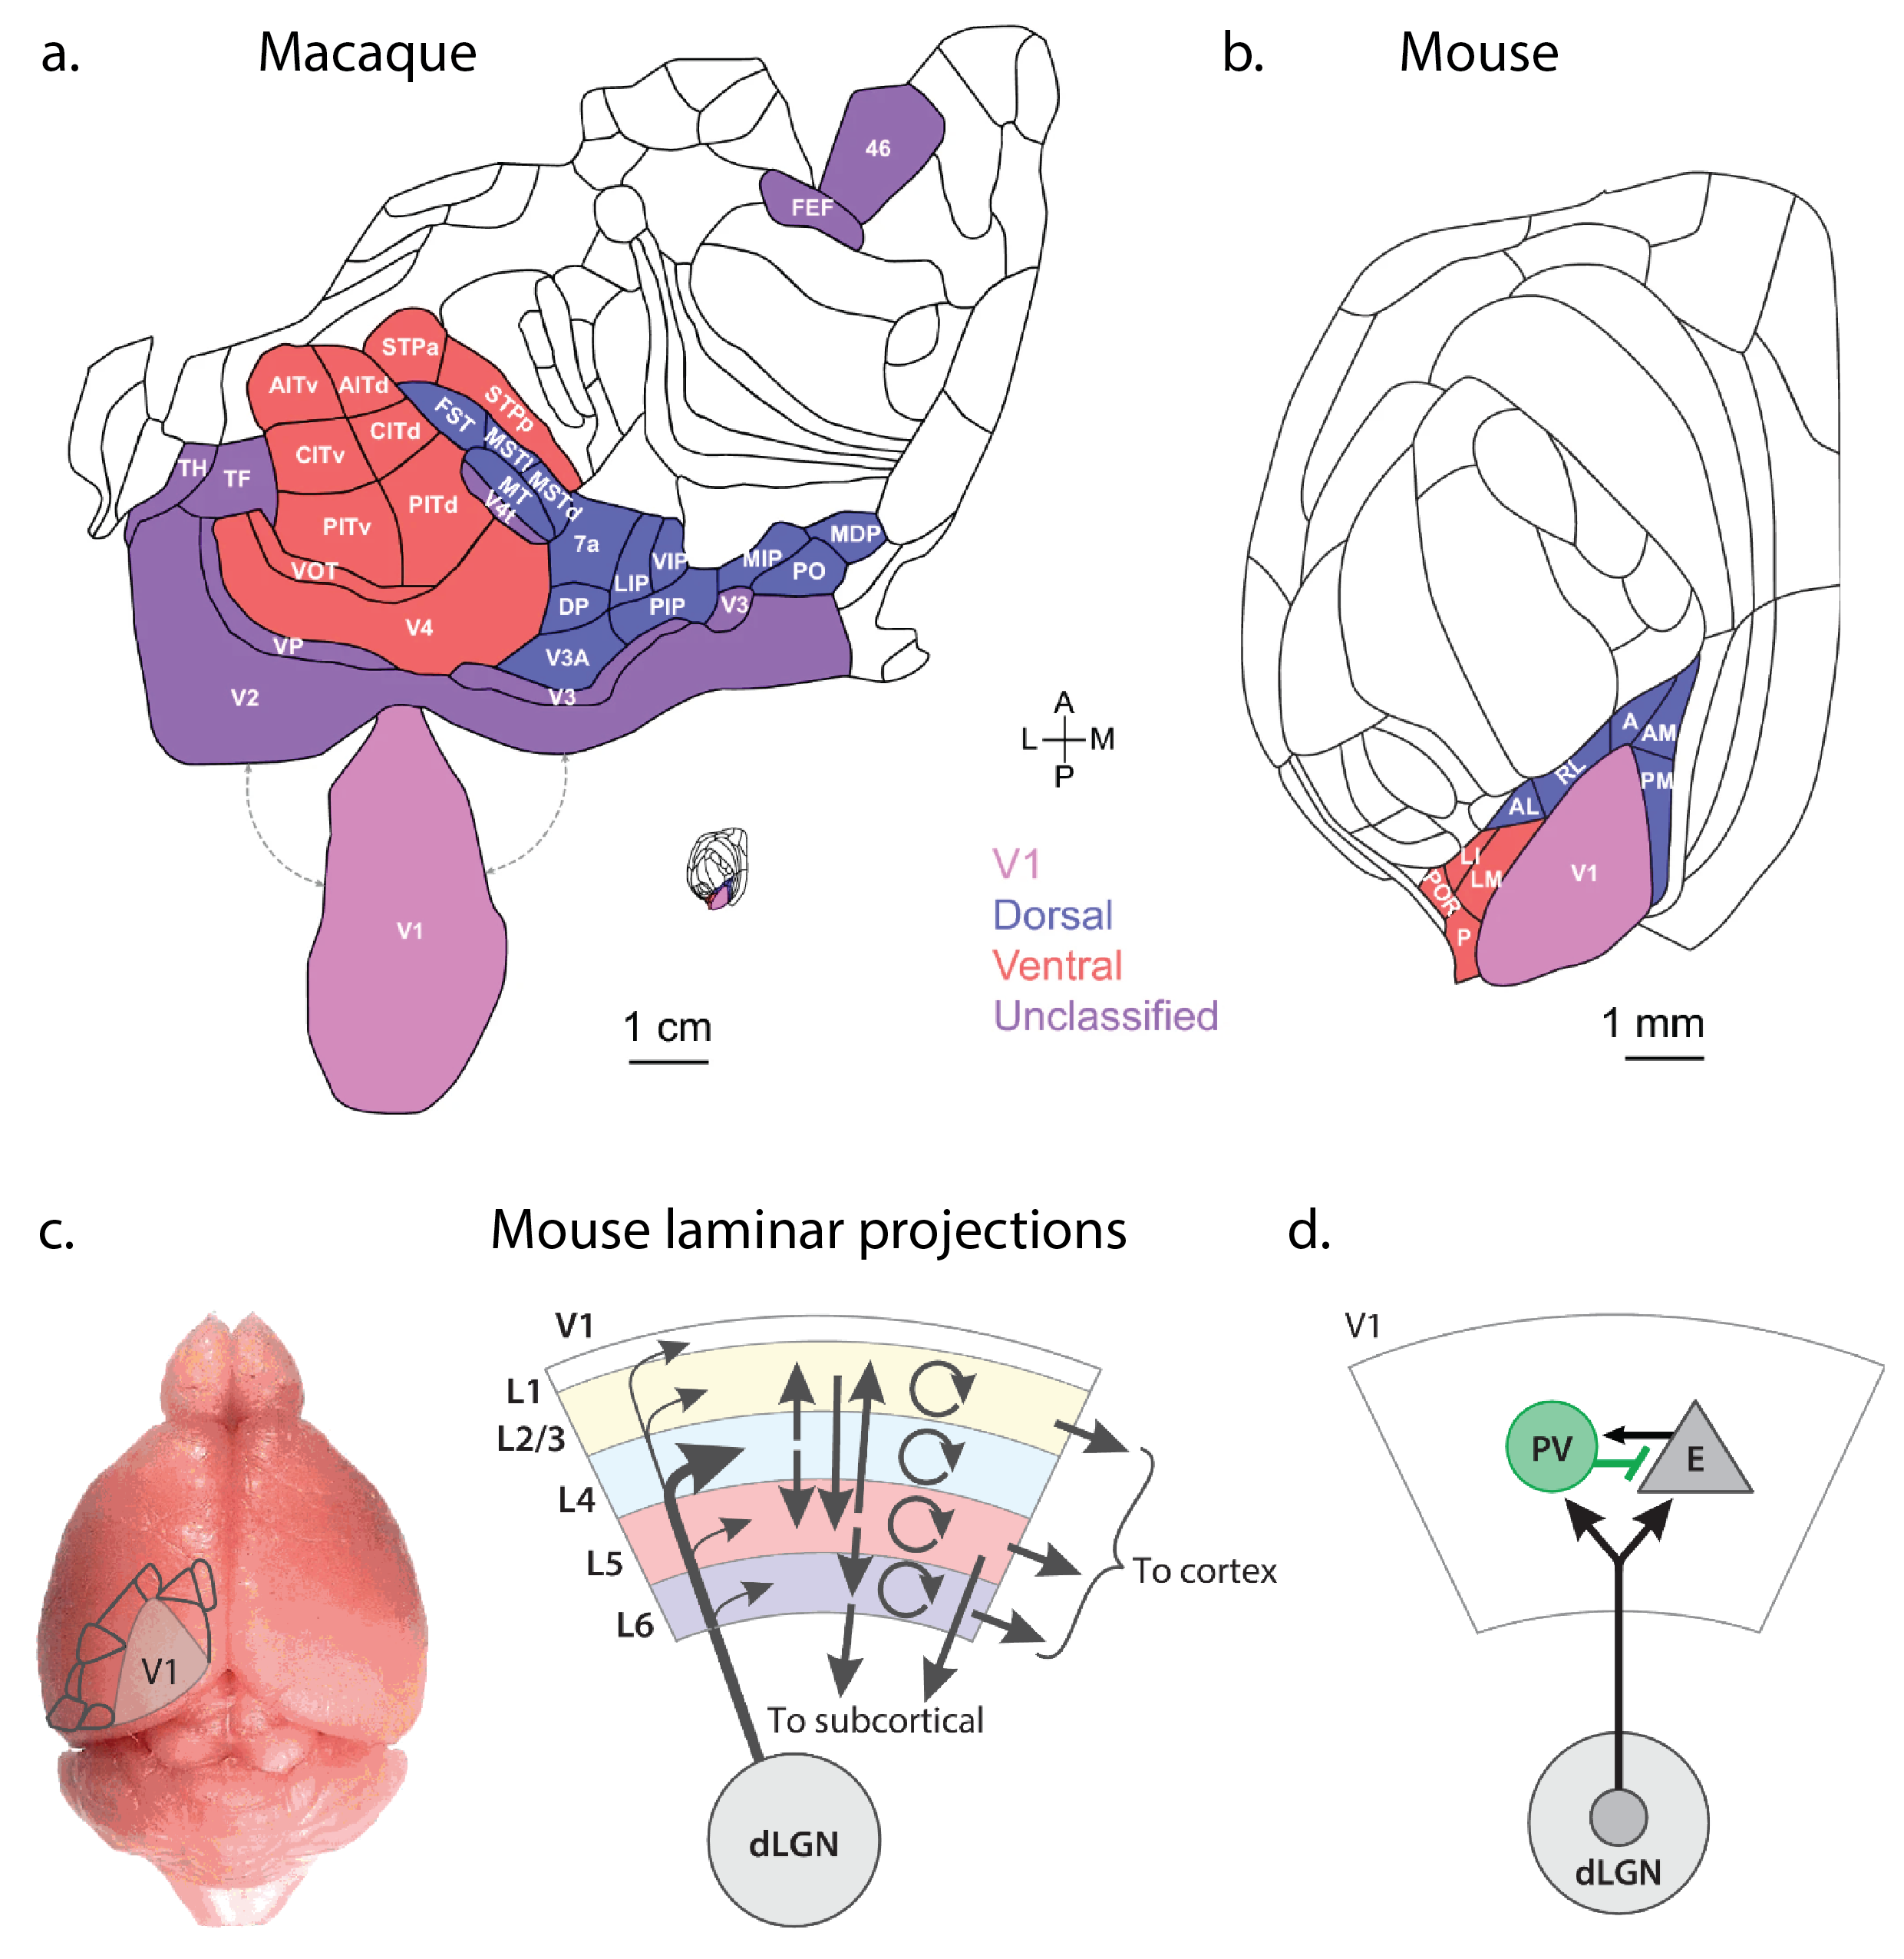
\includegraphics[width=1.0 \textwidth]{adjusted_figures/Laminar_Figure.png}
  \caption{A comparison between the Primate and mouse visual systems. a. The macaque visual system encompasses approximately 30 areas, and therefore, is significantly larger compared to the mouse visual cortex. In the macaque, area V2 wraps around V1 as the secondary visual area. Panel a. adapted from \textcite{gamanutAnatomicalFunctionalConnectomes2022}. b. The mouse visual system, highlighting the dorsal and the ventral stream. Specifically, the ventral area LM is of importance in light of the generation of illusory contours and has been identified as a potential homologue for macaque V2. c. The visual system of the mouse mapped on a cortical image and a description of the laminar projections within V1.  Laminar projections follow a similar pattern to the organisation observed in the macaque. Visual input is relayed from the dorsal lateral geniculate nucleus (dLGN) and is predominantly projected to layer 4, which in turn projects to L2/3 and L5. d. Feedforward input from dLGN to V1 mainly targets excitatory pyramidal cells and PV inhibitory interneurons, indicating that they might be important for the generation of orientation selectivity and the representation of illusion inducer objects. Panels c. and d. adapted from \textcite{niellHowCorticalCircuits2021}}
  \label{fig:Laminar_Figure}
\end{figure}

In both mice and primates the first visual cells sensitive for orientation are found in V1. Both retinal ganglion cells and their target LGN relay cells have circularly symmetric receptive fields and respond to contrast differences within these fields. V1 neurons, however, are responsive to a number of stimulus attributes, such as orientation, motion direction, size, and binocular disparity of visual contours \autocite{hubelReceptiveFieldsBinocular1962}. Early models proposed by \textcite{hubelReceptiveFieldsBinocular1962} emphasised the convergence of signals from the dLGN to V1, suggesting a hierarchical integration of visual information. To test whether orientation selectivity is a strict thalamocortical feedforward process or that these functional properties are a product of neuronal mechanisms on the cortical level \textcite{fersterOrientationSelectivityThalamic1996} inhibited cortical spiking and measured sub-threshold responses. They found that V1 neuron orientation selectivity is largely unaffected by cortical inactivation, providing evidence that the feedforward information transmitted by the LGN relay cells is sufficient to be transformed into orientation selective responses and that cortical circuitry is not required to refine these responses. Despite evidence showing similarities between mammals for how orientation selectivity originates, there are also large differences in the functional organisation across species. For instance, neurons in mouse V1 are not organised in columns with similar orientation preferences, as in primates. Mice also do not have the same pattern of functional segregation by layer that primates exhibit in which simple cells are found more in L4 and complex cells in deeper L2/3 \autocite{martinezReceptiveFieldStructure2005}. Instead, in the mouse, simple and complex cells are evenly distributed across cortical layers \autocite{niellHighlySelectiveReceptive2008}. Nevertheless, these differences in functional organisation are demonstrated to have a minimal impact on the functional properties of orientation tuning \autocite{hooserOrientationSelectivityOrientation2005}. 

Physiologically, V1 neurons can be described as simple or complex cells and are both orientation selective \autocite{skottunClassifyingSimpleComplex1991}. Simple cells receive direct input from the dLGN relay cells and their receptive field responses are characterised by segregated ON and OFF fields that prefer light or dark input, respectively. These subfields are elongated taking on an elliptical shape along the axis of the neuron's preferred orientation. Due to the segregated ON and OFF subfields their responses are sensitive to changes in phase and polarity \autocite{mechlerClassificationSimpleComplex2002}. In contrast, complex cells that receive input from V1 simple cells have receptive fields in which ON and OFF regions are not spatially segregated. Therefore, complex cells respond to both increases and decreases in luminance at the same location and are not sensitive to stimulus polarity or tuned to a particular phase. An important question is how the spatial offset of ON and OFF subfields are developed, since these pathways are not segregated within the LGN. \textcite{nguyenModelOriginDevelopment2019} demonstrated that through a process of Hebbian learning the ON and OFF inputs could be sufficiently segregated to produce orientation selective neurons. In their simulations they simulated a 6 x 6 degree patch of visual field and within this field randomly distributed ON and OFF channels. Then they stimulated neuronal responses using a drifting grating over the full range of orientations. Each cycle in the development process then consisted of increasing the weights of all synapses for one randomly chosen subcortical channel. If the firing rate of a cortical neuron increased as a result, the synapse between the channel and the cortical target remained strengthened, and was otherwise decreased. After roughly 16000 cycles they found segregated ON and OFF subfields that were sufficient for orientation tuning.
\bigbreak

% Need to rewrite this to fit the description of the figure.
This leads us into an examination of various models that attempt to explain how the visual system integrates local and global information to have a shape or contour emerge from inducer shapes. The abutting grating and Kanizsa illusions are both characterised by congruent illusory inducing points, identifiable by the presence of aligned line endings. Kanizsa inducers are considered more complex than abutting line inducers because each inducer point forms part of a corner, essentially two line ends meeting at an angle. In contrast, the abutting grating illusion is simpler, since its inducer points consist of horizontal lines. The inducer lines could be represented by individual length sensitive endstopped neurons, first classified by \textcite{hubelRECEPTIVEFIELDSFUNCTIONAL1965} in the cat's primary visual cortex. These cells are orientation-tuned and exhibit inhibition when a line segment exceeds their excitatory receptive field into their inhibitory end zone \hyperref[fig:endstop_mechanism]{figure 3a}. Subsequent research revealed that a significant portion of V1 simple and complex neurons exhibit endstopping to varying degrees across different species, including primates, cats, and mice \autocite{deangelisLengthWidthTuning1994,jonesSurroundSuppressionPrimate2001,sceniakVisualSpatialCharacterization2001}. Computational models expanded on these findings by demonstrating that through the integration of endstopped cells feedback responses could induce illusory neural activity. A cortical mechanism that was proposed can bee seen in \hyperref[fig:endstop_mechanism]{figure 3 b}. Multiple endstopped cells are connected to a gating mechanism (X cells), which only transmits a signal when both cells are active. These endstopped signals are then summed in a higher visual area and through feedback an orthogonal illusory response is generated \autocite{vonderheydtIllusoryContoursCortical1984}. The neuron in the higher visual area has been described as a bipole cell \textcite{grossbergRoleIllusoryContours1987}.  Bipole cells are sensitive to the collinear alignment of edges in local boundary detection and are capable of integrating the output of endstopped cells to complete open boundaries. In these frameworks recurrent activity ultimately fills in the illusory contour. This type of activity is typically not present in deep neural networks (DNN). As a result, it is not surprising that feedforward DNNs fail in boundary completion tasks \autocite{fanChallengingDeepLearning2023}.  

\begin{figure}[H]
  \centering
  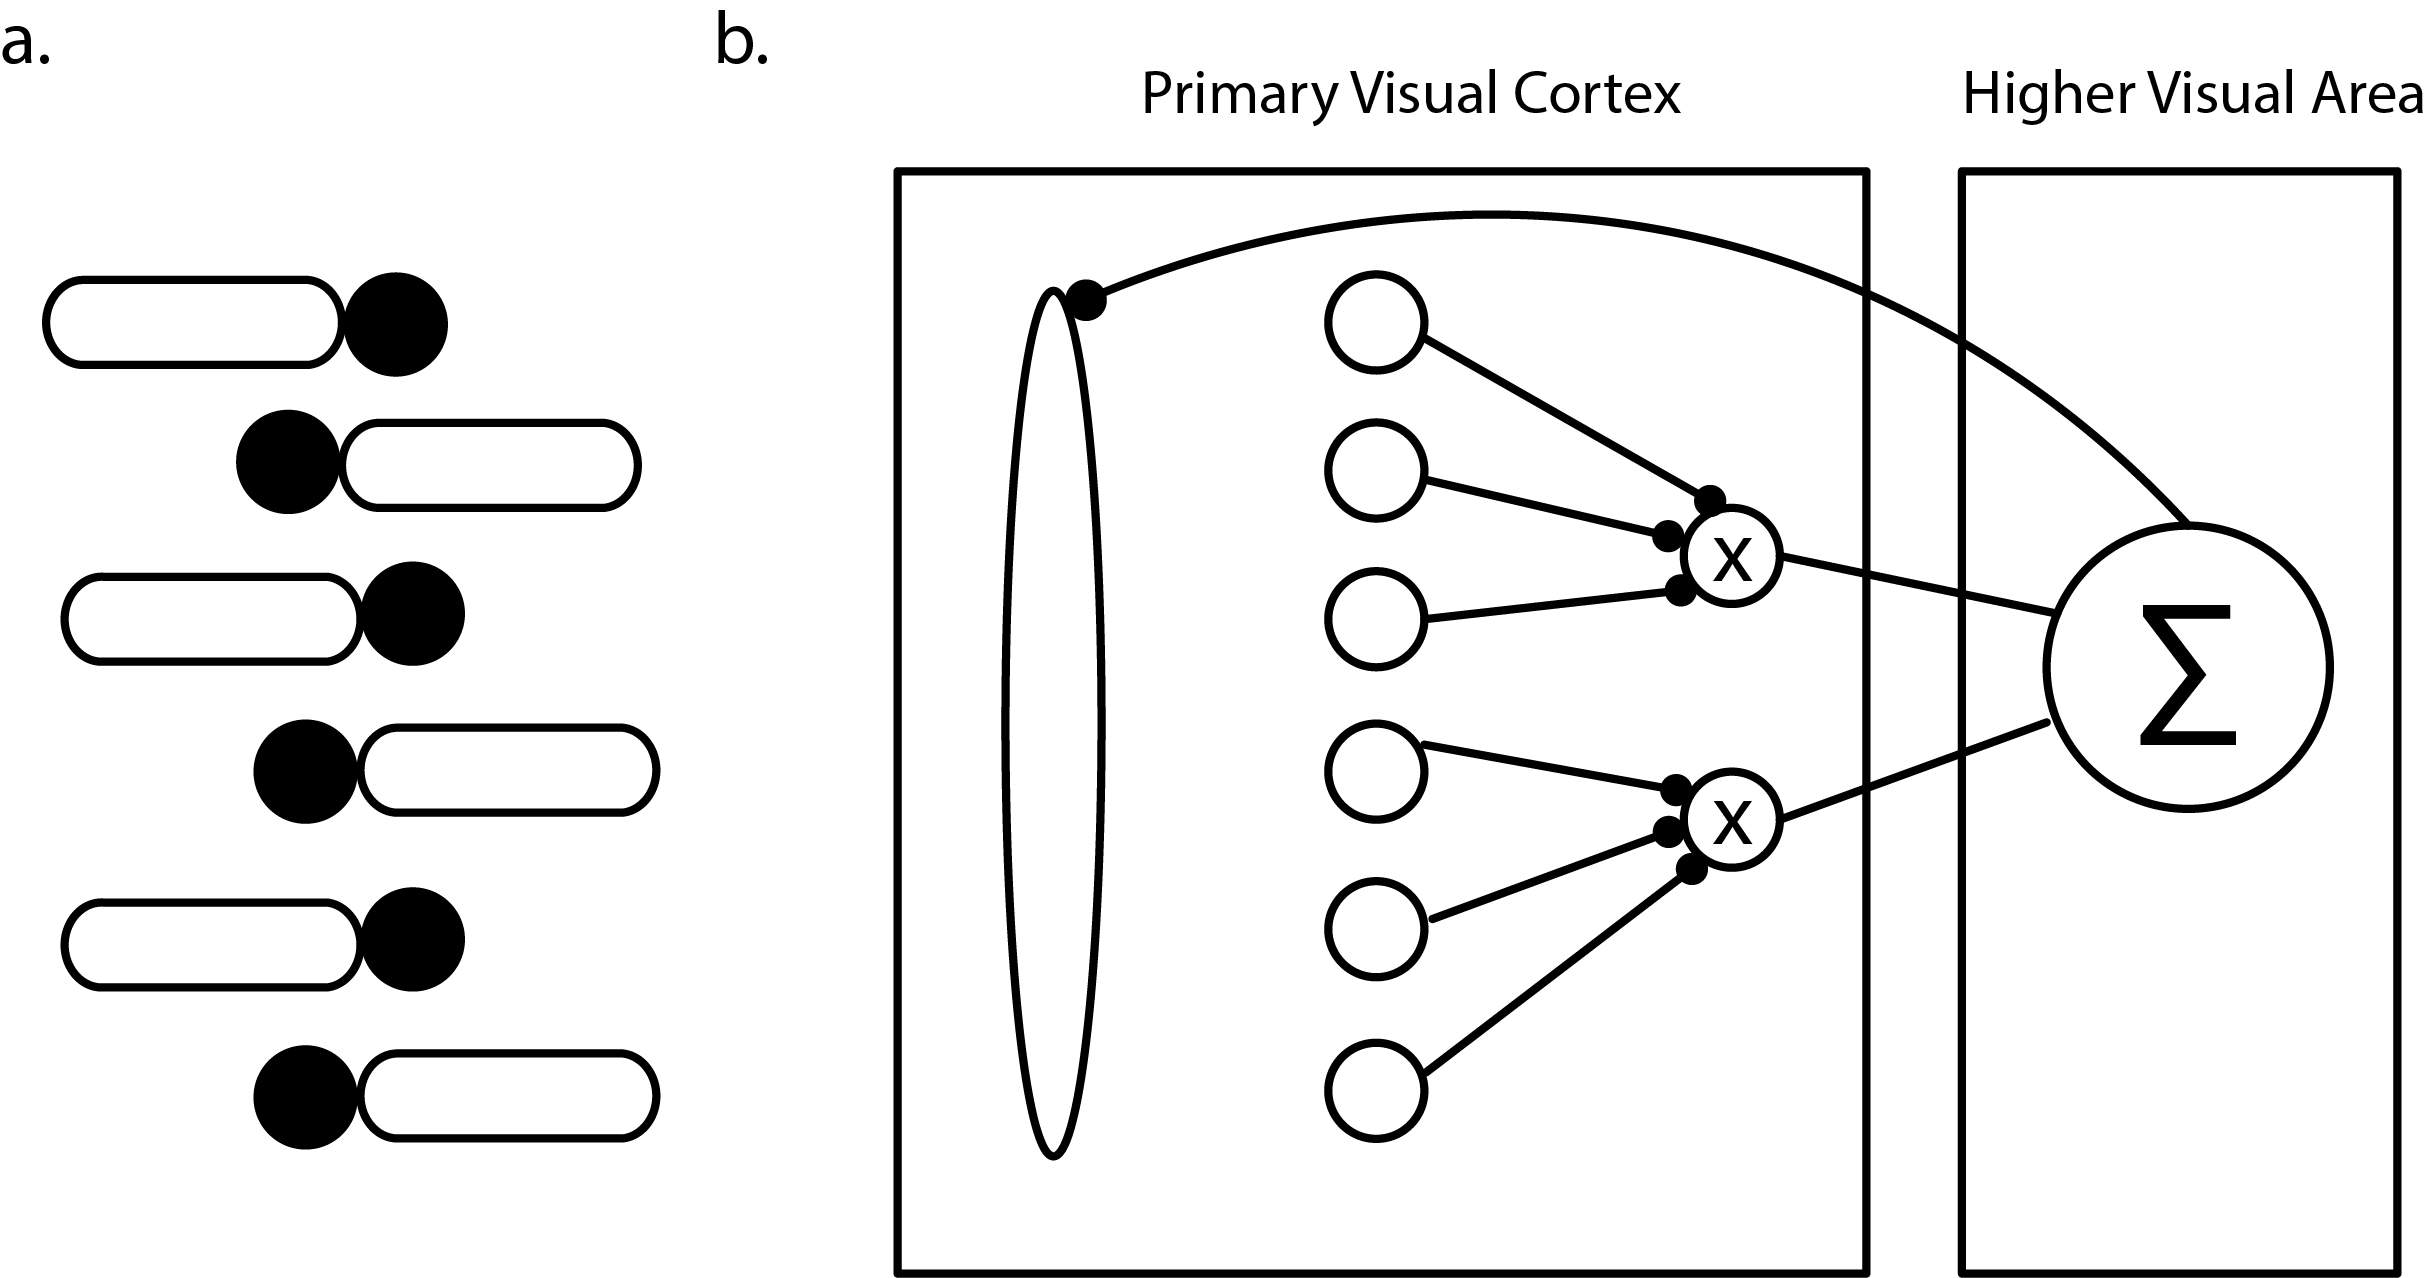
\includegraphics[width=1.0 \textwidth]{adjusted_figures/endstop_mechanism.png}
  \caption{The proposed architecture for the representation of illusory contours in primary visual cortex. a. The receptive field characteristics of an endstopped cell. The elongated white receptive field is the excitatory zone. If a contour fitting the preferred orientation of the endstopped cell falls onto this excitatory zone, the firing rate increases. However, when the stimulus is longer and extends into the black zone of the receptive field, the firing rate is decreased. b. A proposed integration mechanism from \textcite{vonderheydtIllusoryContoursCortical1984}. It describes how the endstopped cells can be integrated in cells that form a logic gate. When both cells are active they project a signal to higher visual area that projects feedback information to lower visual area V1. The feedback creates the V1 activation of cells that respond to the orientation of the illusory contour and not the inducer orientation.}
  \label{fig:endstop_mechanism}
\end{figure}

%%%%%%%%%%%%%%%%%old good text
%ToDo integrate with the figure for recurrent completion
% \Textcite{vonderheydtMechanismsContourPerception1989} expanded on these ideas by demonstrating that endstopped cells in the visual cortex, particularly in V1 and V2 areas, respond to lines and edges, contributing to the perception of illusory contours through mechanisms that integrate local orientation signals into coherent shapes \autocite{grossbergTextureSegregationSurface1998}. These endstopped neurons are maximally activated when lines or edges terminate within their receptive field but deactivate when the lines extend through it, making them crucial for detecting terminations and corners, fundamental elements in creating the perception of contours. \textcite{grossbergRoleIllusoryContours1987} highlights the need for another cell type, the bipole cell. Bipole cells are sensitive to collinear alignment of edges in local boundary detection, they are capable of integrating the output of endstopped cells and can be used to complete open boundaries. Higher visual areas such as V2 and V4 are necessary for integrating information over larger spatial ranges and bridging gaps between endstopped points. These areas use feedback connections to complex cells in earlier visual areas, reinforcing and refining the initial boundary signals to create stable and coherent perceptions of illusory contours.
% \begin{figure}[H]
%   \centering
%   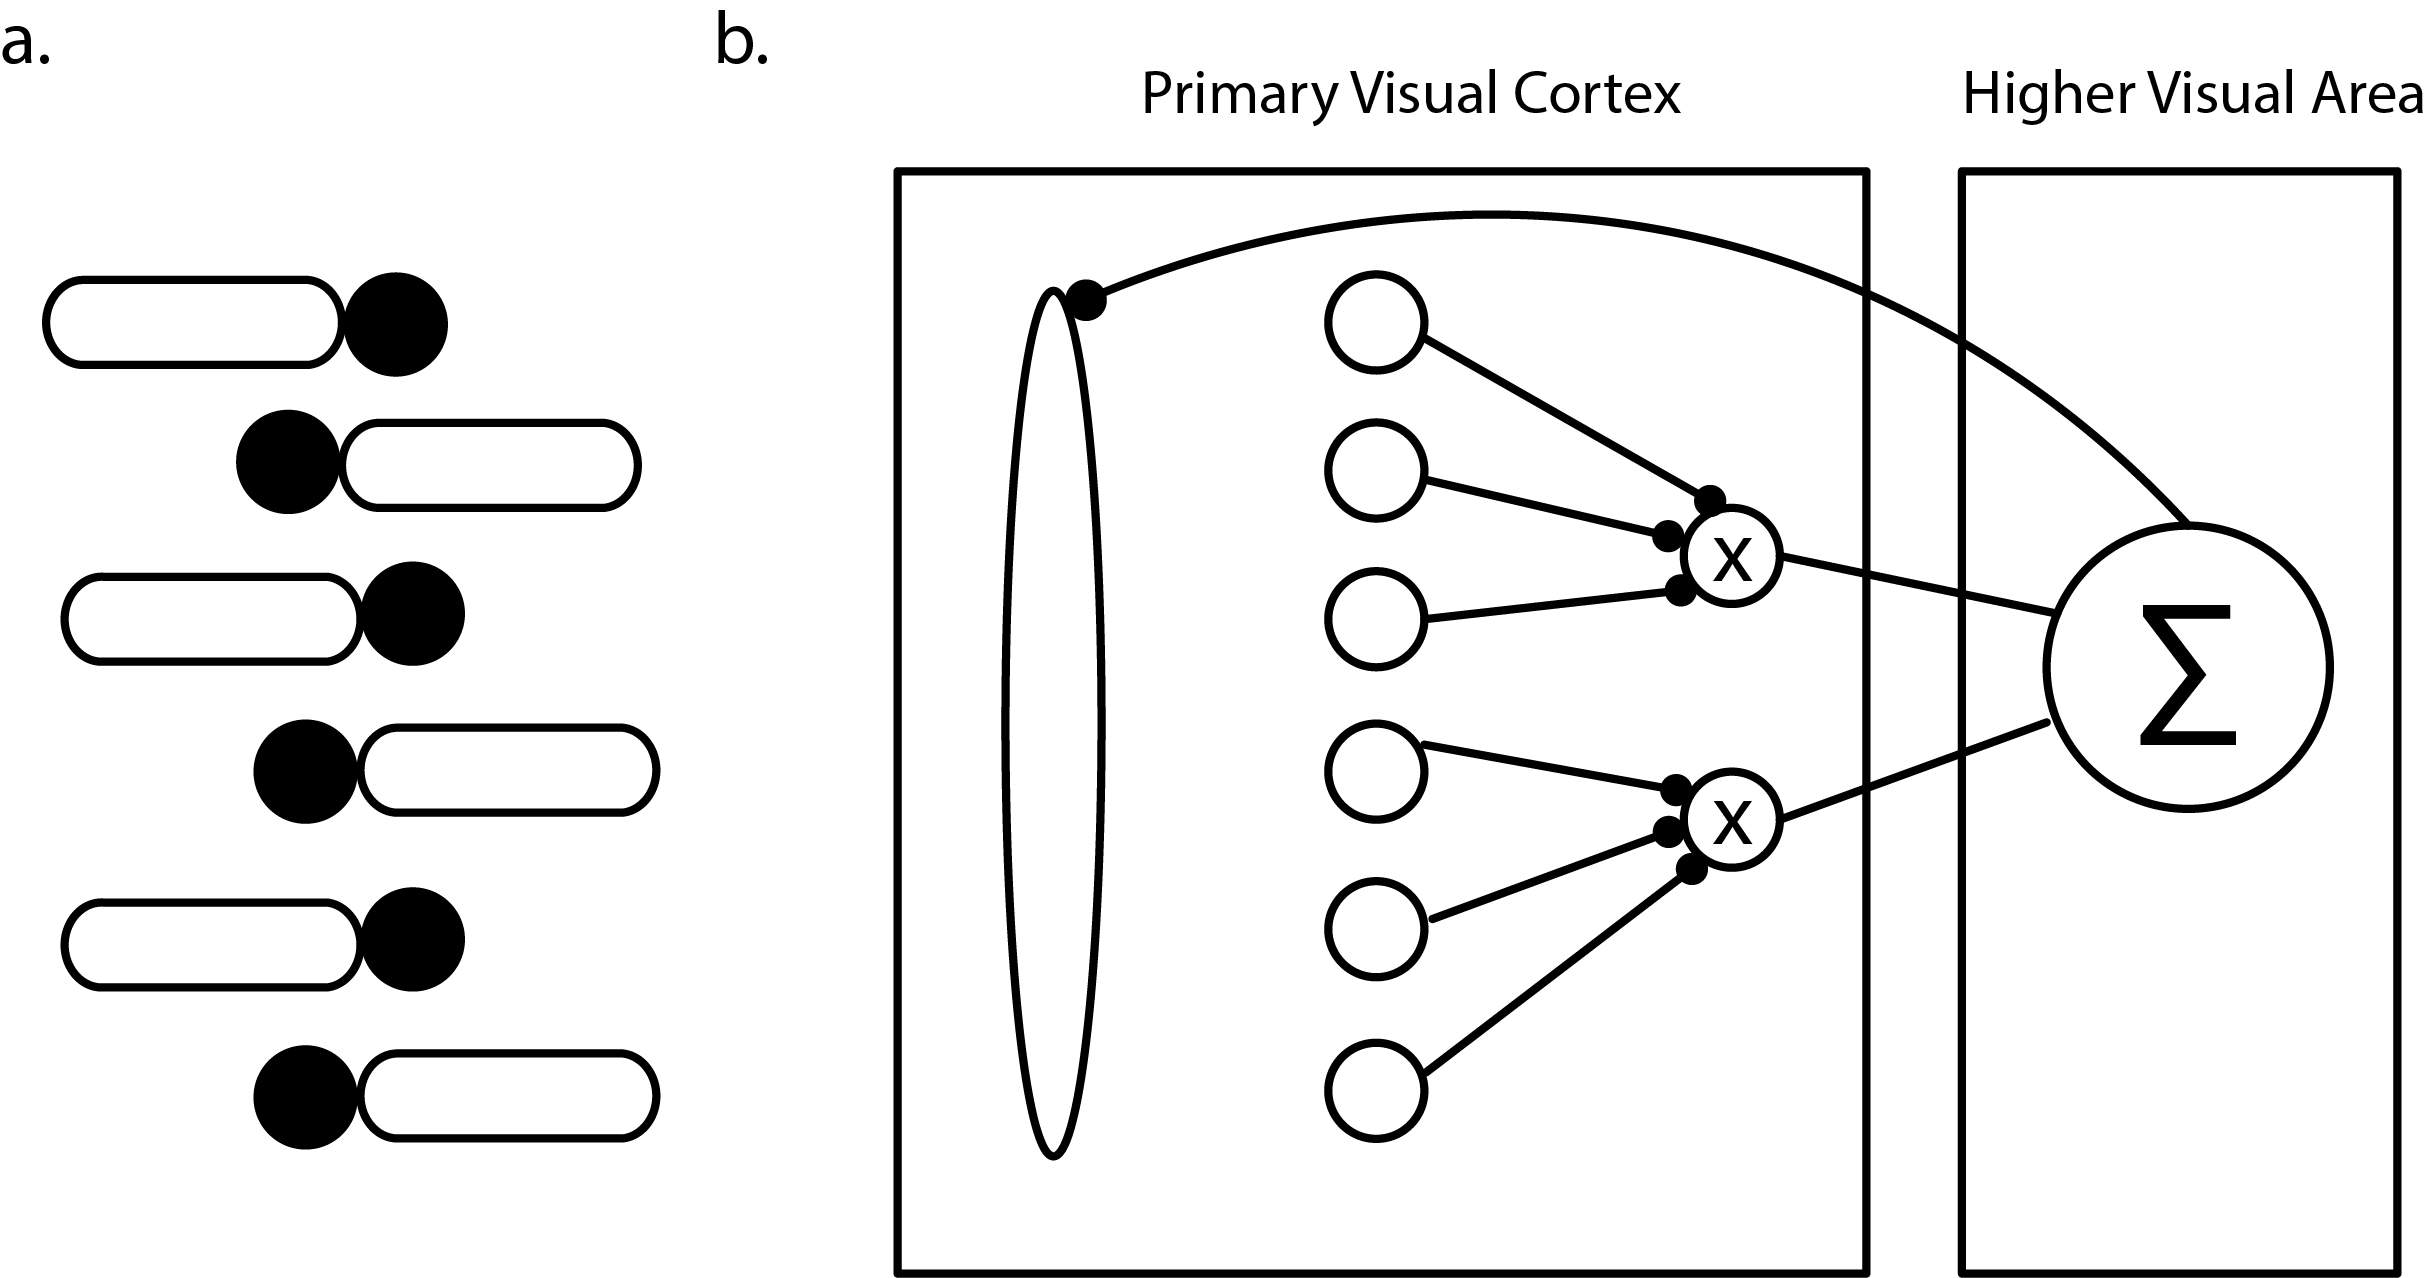
\includegraphics[width=1.0 \textwidth]{adjusted_figures/endstop_mechanism.png}
%   \caption{The proposed architecture for the representation of illusory contours in primary visual cortex. a. The receptive field characteristics of an endstopped cell. The elongated white receptive field is the excitatory zone. If a contour fitting the preferred orientation of the endstopped cell falls onto this excitatory zone, the firing rate increases. However, when the stimulus is longer and extends into the black zone of the receptive field, the firing rate is decreased. b. A proposed integration mechanism from \textcite{sorianoAbuttingGratingIllusion1996}. It describes how the endstopped cells can be integrated in cells that form a logic gate. When both cells are active they project a signal to higher visual area that projects feedback information to lower visual area V1. The feedback creates the V1 activation of cells that respond to the orientation of the illusory contour and not the inducer orientation.}
%   \label{fig:endstop_mechanism}
% \end{figure}

% A recent study by \textcite{fanChallengingDeepLearning2023} explores the challenges deep neural networks (DNNs) face in representing illusory contours, specifically through the abutting grating illusion. Illusory contours, such as those seen in the abutting grating illusion, evoke perceptions of boundaries where none exist, a phenomenon that standard edge detectors cannot handle. The study highlights the failure of convolutional neural networks (CNNs) in revealing activity along these contours and proposes that recurrent processing, akin to that in biological vision, is crucial for accurate representation.

% In biological systems, recurrent connections allow for the integration of contextual information, essential for resolving ambiguities and ensuring consistent perceptual grouping and boundary completion. DNNs, which lack such recurrency, often fail in tasks involving illusory contours, underscoring a significant gap between artificial and biological vision systems \autocite{fanChallengingDeepLearning2023}. Other models that follow a more biologically plausible architecture with recurrent connections have more success regarding the representation of illusory contours \autocite{grossbergRoleIllusoryContours1987,vonderheydtMechanismsContourPerception1989}. Their models incorporate endstopping cells as part of the boundary contour system (BCS) and bipole cells as part of the feature contour system (FCS) to simulate how the brain perceives continuous boundaries from fragmented visual information. Grossberg and Mingolla's neural dynamics model, for instance, shows how these BCS and FCS can interact with each other and through feedback loops complete boundaries and surfaces. The endstopped cell would code for a particular boundary ending of a line and the bipole cells would integrate these termination signals, this interaction is critical for the perception of illusory contours and shapes \autocite{grossbergTextureSegregationSurface1998}. However, while bipole cells and endstopped neurons play crucial roles in local boundary detection, the full representation of illusory contours requires a more integrated approach involving higher visual areas and recurrent processing. This hierarchical and recursive processing framework enables the visual system to perceive complex shapes and contours that are not explicitly present in the visual input, a sophistication that current DNNs lack.
%%%%%%%%%%%%%%%%%%%%%%old good text



% A recent study by \textcite{fanChallengingDeepLearning2023} explores the challenges deep neural networks (DNNs) face in representing illusory contours, specifically through the abutting grating illusion. Illusory contours, such as those seen in the abutting grating illusion, evoke perceptions of boundaries where none exist, a phenomenon that standard edge detectors cannot handle. The study highlights the failure of convolutional neural networks (CNNs) in revealing activity along these contours and proposes that recurrent processing, akin to that in biological vision, is crucial for accurate representation. In biological systems, recurrent connections allow for the integration of contextual information, essential for resolving ambiguities and ensuring consistent perceptual grouping and boundary completion. DNNs, which lack such recurrency, often fail in tasks involving illusory contours, underscoring a significant gap between artificial and biological vision systems \autocite{fanChallengingDeepLearning2023}. 

% Other models that follow a more biologically plausible architecture with recurrent connections have more success regarding the representation of illusory contours \autocite{grossbergFillingInFormsSurface2003,vonderheydtMechanismsContourPerception1989}. Their models incorporate endstopping cells as part of the boundary contour system (BCS) and bipole cells as part of the feature contour system (FCS) to simulate how the brain perceives continuous boundaries from fragmented visual information. Grossberg and Mingolla's neural dynamics model, for instance, shows how these BCS and FCS can interact with each other and through feedback loops complete boundaries and surfaces. The endstopped cell would code for a particular boundary ending of a line and the bipole cells would integrate these termination signals, this interaction is critical for the perception of illusory contours and shapes \autocite{grossbergTextureSegregationSurface1998}. 

% Peterhans and von der Heydt expanded on these ideas by demonstrating that endstopped cells in the visual cortex, particularly in V1 and V2 areas, respond to lines and edges, contributing to the perception of illusory contours through mechanisms that integrate local orientation signals into coherent shapes \autocite{grossbergTextureSegregationSurface1998}. These endstopped neurons are maximally activated when lines or edges terminate within their receptive field but deactivate when the lines extend through it, making them crucial for detecting terminations and corners, fundamental elements in creating the perception of contours. \textcite{grossbergFillingInFormsSurface2003} highlights the need for another cell type, the bipole cell. Bipole cells are sensitive to collinear alignment of edges in local boundary detection, they are capable of integrating the output of endstopped cells and can be used to complete open boundaries. Higher visual areas such as V2 and V4 are necessary for integrating information over larger spatial ranges and bridging gaps between endstopped points. These areas use feedback connections to complex cells in earlier visual areas, reinforcing and refining the initial boundary signals to create stable and coherent perceptions of illusory contours.

% However, while bipole cells and endstopped neurons play crucial roles in local boundary detection, the full representation of illusory contours requires a more integrated approach involving higher visual areas and recurrent processing. This hierarchical and recursive processing framework enables the visual system to perceive complex shapes and contours that are not explicitly present in the visual input, a sophistication that current DNNs lack.
\bigbreak
Despite these computational insights, neurophysiological studies have largely overlooked how endstopping is integrated into higher visual areas for illusory contour perception. Previous computational simulations, while informative, have relied on feed-forward convolutions without accounting for biological constraints, such as the lack of direct inhibition observed in physiological endstopping \autocite{sillitoContributionExcitatoryInhibitory1977} and the absence of feedback mechanisms now recognised as crucial for the representation of illusory contours in lower visual areas \autocite{pakTopDownFeedbackControls2020}. Addressing this gap, our current research endeavours are to (1) simulate the minimal circuit necessary for stable endstopping using leaky integrate and fire (LIF) neurons and (2) integrate endstopped microcircuits through population rate models to accurately represent the abutting grating illusion in line with physiology. Our findings identify the cell types necessary to exhibit endstopping characteristics and clarify how the orientation selectivity of endstopped cells in higher visual areas modulates the representation of illusory contours through recurrent activity. By incorporating endstopped cells into a hierarchical model, we aim to elucidate the neural mechanisms underlying illusory contour perception and provide a comprehensive understanding of how the visual system processes these contours across species.

\newpage
\section*{Methods}
% Introduction that states that we used two models with a rationalisation of why
%\subsection{Point neuron model and population neuron model.}
To investigate the minimal circuit necessary for endstopping and its role in generating illusory contours within the visual cortex of the mouse, the current study used two distinct computational frameworks. In the initial phase of the investigation, the utilised LIF models allowed us to simulate the spatial and temporal integration of synaptic input, at the single-cell level. This approach provided a foundational circuitry for orientation selectivity, complex cell features such as polarity invariance, and length tuning. However, the current connectivity between LIF cells was set manually, and the complexity and computational demands associated with the tuning of each neuron required the current study to shift towards population models for the subsequent phase. Moreover, this phase focused on the generation of illusory contour responses through feedforward and feedback interactions. Nevertheless, the LIF network allowed us to estimate the necessary number of cells and the connectivity between them required to create a stable neural mechanism for endstopping. The population models could then abstract this behaviour into a computationally tractable form, enabling efficient simulation of illusory contour generation throughout the visual hierarchy. 


%\subsection{Simulating the Local microcircuit for Endstopping.}
To create the network for generating endstopping behaviour, the Brain Modelling Toolkit (BMTK) was used. We initialised an instance of the NetworkBuilder class provided by BMTK to construct an architecture of spiking point neurons, creating networks for both the dLGN and V1. Then visual stimuli were presented through a three-dimensional array format (t, y, x), with each entry along the first dimension (time, t) representing a frame, and input organised along the vertical (y) and horizontal (x) dimensions. The BMTK simulation pipeline processed visual information through a series of steps reflecting the increase in neural complexity of the visual system. The toolkit allowed for precise control over the spatial arrangement and connectivity of neurons, facilitating the modelling of user specified neural circuits and their functional behaviours.

An important aspect of the BMTK is the segregation of the visual field as input and neural space. The BMTK has an input network called Filternet that generates firing rates from contrast present in the visual field. This effectively simulates the transformation from light intensity to neural signals as is done by the retina in visual system. Furthermore, the filter cells used in Filternet are responsive to either black or white light intensities thereby simulating the filtering properties of the dLGN, serving as spiking input to the cortex. This simulation environment allows for detailed analysis of how dLGN neurons process various visual inputs and contribute to the overall neural activity in V1. V1 was simulated via a framework called Pointnet, which simulated point neuron networks within the NEST environment. NEST is well-suited for modelling point neural networks and supports the integration of predeveloped point-neuron models. This approach enabled the modelling of cortical processing of visual information, where the integration of inputs from the dLGN and the cortical circuitry results in the emergence of visual features such as orientation selectivity \hyperref[fig:LIF_Overview]{(Figure 4a)}, phase invariance \hyperref[fig:LIF_Overview]{(Figure 4a)}, and length tuning \hyperref[fig:LIF_Overview]{(Figure 4c)}. By separating the simulations into Filternet for the dLGN and Pointnet for the V1 cortex, we had control over the thalamocortical transformation required for orientation selectivity, and guarantee the analysis at the appropriate level of detail.
\bigbreak

% Overview figure
\begin{figure}[H]
  \centering
  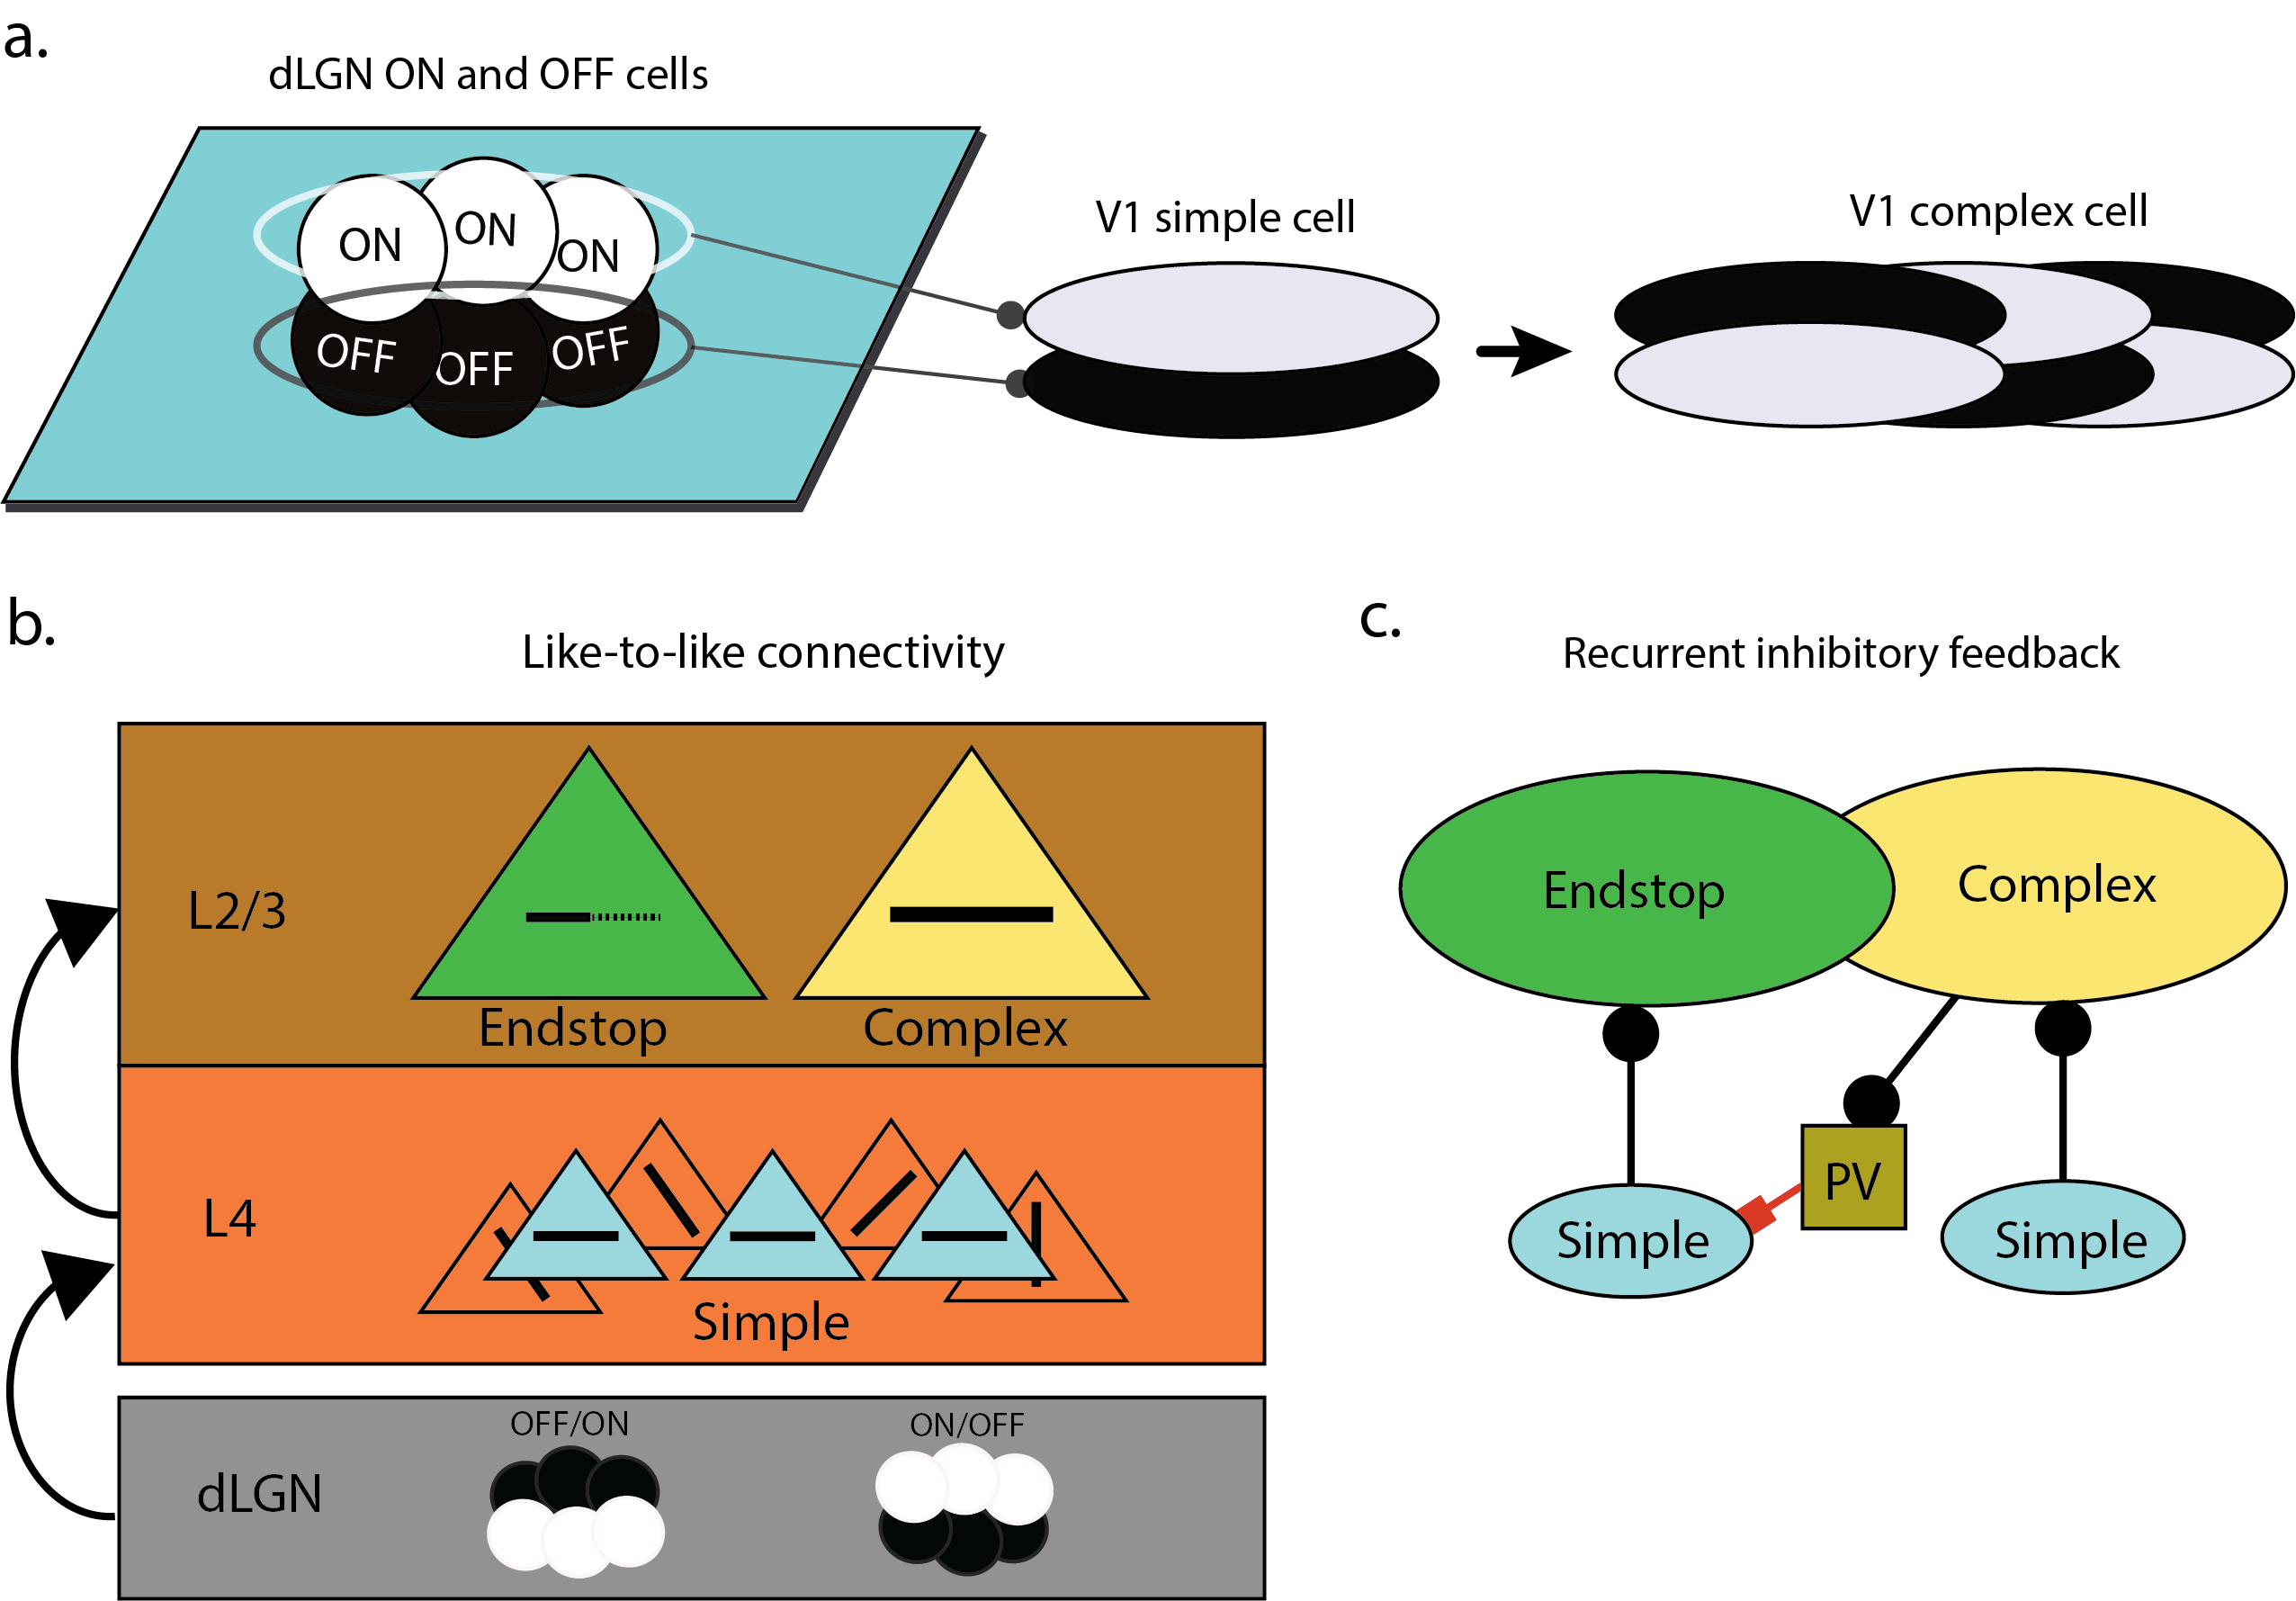
\includegraphics[width=1.0 \textwidth]{adjusted_figures/LIF_Overview_Receptive_Field_Methods.png}
  \caption{The generation of endstopped simple and complex cells through a recurrent inhibitory feedback microcircuit. a. The dLGN ON and OFF cells converge with a spatial offset onto a simple cell, creating a simple filter that responds to edges. Combining multiple simple cells with overlapping ON and OFF fields creates a complex cell. The complex cells, due to their overlapping subfields are not dependent on stimulus polarity and are phase invariant. b. A diagram showing the hierarchical complexity of cells that are connected based on their orientation tuning. The green endstopped cell is illustrated by a dotted line end, showing that an extended line end will result in a decreased firing rate. c. Shows how a particular endstopped microcircuit is made. Population of simple cells converge onto the endstopped and complex cell to give them feedforward input. However, if a line would extend over the endstopped receptive field, it will stimulate the complex cell. A recurrent inhibitory feedback loop would then inhibit the simple population that is responsible for the endstopped cell's drive and firing will decrease.}
  \label{fig:LIF_Overview}
\end{figure}

% ToDo: make sure no redundant information is in it. 
%\subsection{dLGN transformes light intensity to neural activity.}
The first relay station in the visual pathway is the dLGN, which receives input from the retina and transmits visual information to V1 for further processing. The dLGN processes visual stimuli through two distinct pathways: the ON and OFF pathways, which respond to increases and decreases in light intensity, respectively. These pathways are essential for encoding contrast and edge information in visual scenes, providing the initial processing steps that shape the neural representation of visual stimuli. By presenting visual stimuli to the dLGN network, we can effectively simulate the translation of light input into neural signals, creating the first layer for contrast detection in the visual system. Since we are interested in contrast, which is encoded in V1 rather than colour, only monochromatic greyscale stimuli were shown. To transform this input array into neural signals, the dLGN was simulated as a linear-non-linear Poisson cascade model. First, visual input within the space of the receptive field of the dLGN cell is convolved with a linear filter. Then a nonlinear function is applied to the output of the previous linear filter, giving the neuron's instantaneous spike rate as its output. Finally, this firing rate generates spikes according to an inhomogeneous Poisson process \autocite{moskovitzComparisonDeepLearning2018}. The current dLGN model consists of two unit types, ON and OFF surround cells, optimised to closely mimic mammalian thalamic cells \autocite{billehSystematicIntegrationStructural2020}. The ON and OFF cells of the LGN converge on a layer of simple cells, effectively exciting L4 of V1 (Figure \ref{fig:LIF_connectivity}a). This dual pathway of ON/OFF cells is essential for the initial segregation of visual information, setting the stage for more complex edge detection and contrast processing within higher cortical areas. We analysed spiking features in response to static images. Therefore, we focused on modeling ON and OFF cells to have a predominantly sustained responses (sON and sOFF). We used the model templates in our node configuration to implement these cells in our network. The parameters for these cells were set based on values derived from electrophysiological recordings from the mouse dLGN, as reported by \textcite{durandComparisonVisualResponse2016} and \textcite{billehSystematicIntegrationStructural2020}.

\begin{figure}[H]
  \centering
  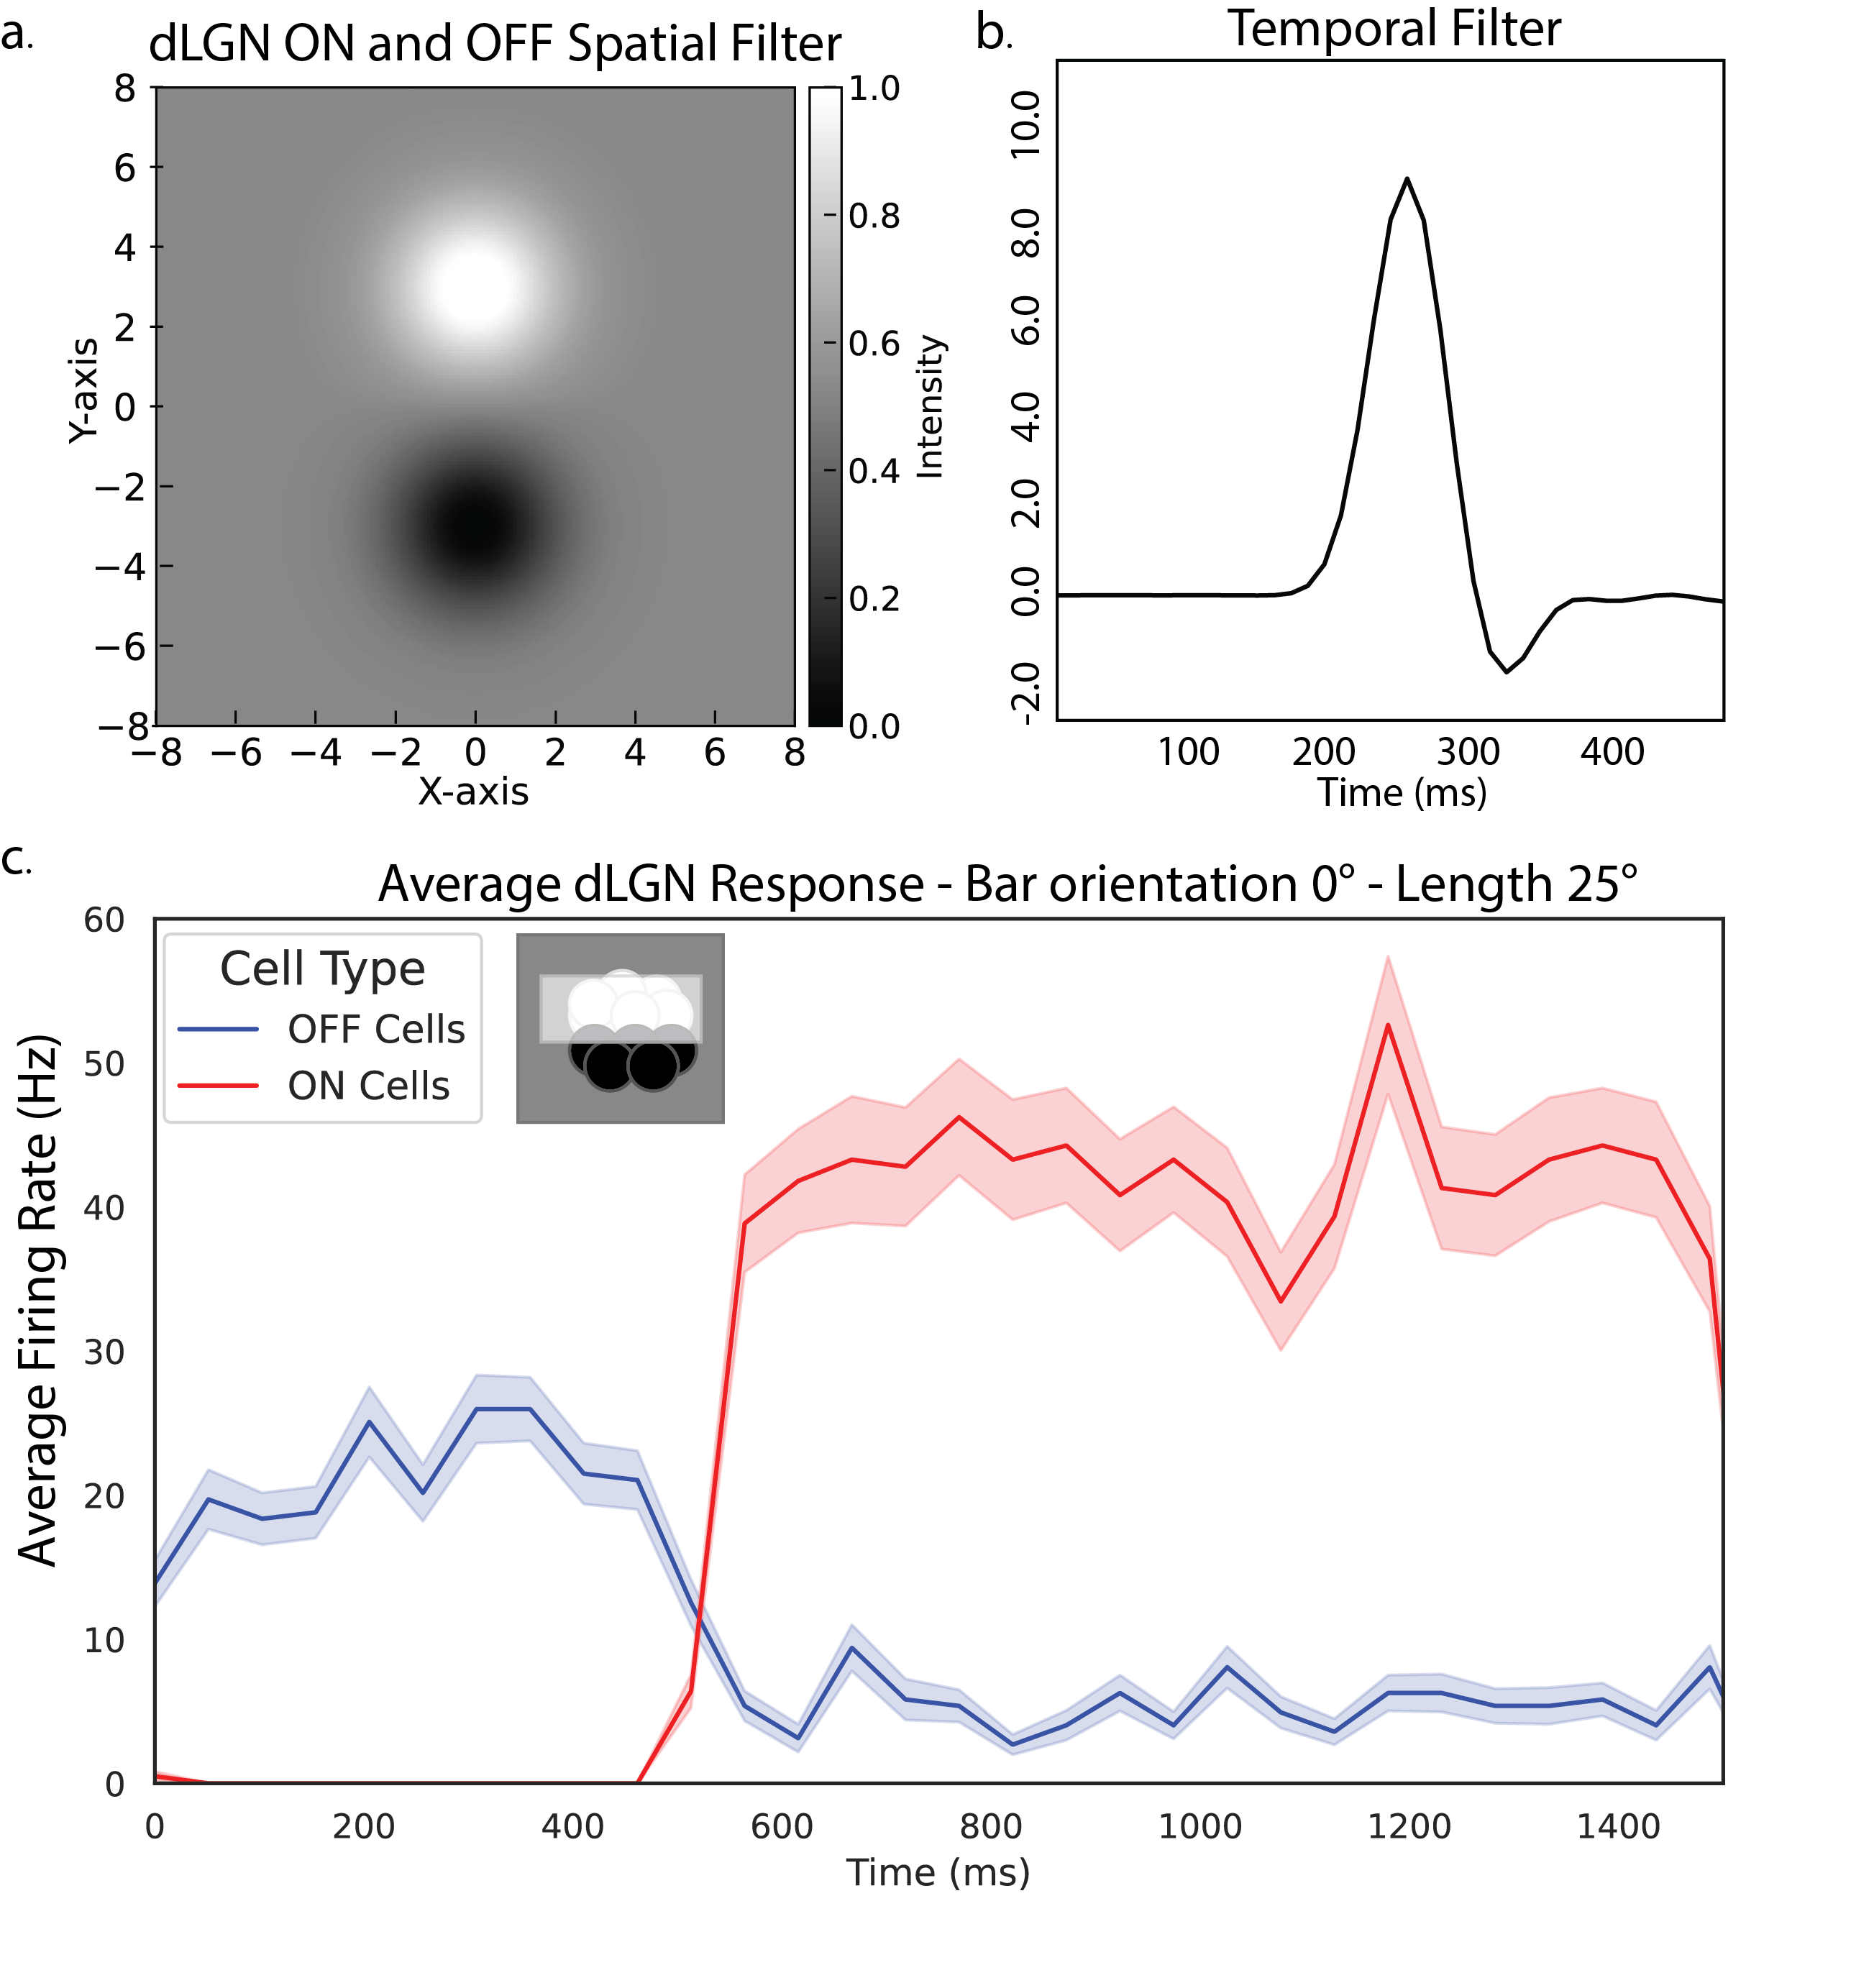
\includegraphics[width=1.0 \textwidth]{adjusted_figures/lgn_response_fig.png}
  \caption{On and OFF cells in the dorsal lateral geniculate nucleus. a. The ON and OFF spatial filters used as input to V1 simple cells. The ON and OFF filters are two inverted gaussian functions that are sensitive to bright and dark input, respectively. b. Each filter also has a temporal filter that dictates how the response changes through time. c. The ON and OFF response to a bar that is completely exciting the ON cells as well as some minor stimulation to the OFF cells. The stimulus is a bar with a length of 25 visual degrees and is horizontal with a rotation of 0 degrees. All stimuli presented to the dLGN were monochromatic and activated ON or OFF cells.}
  \label{fig:LIF_connectivity}
\end{figure}

For the spatial filtering of the dLGN receptive fields, we employed a Gaussian filter characterised by its spatial size and rotation. The default spatial size was set to 5.0 spatial degrees, which means the filter covered a 5-degree area in both the horizontal and vertical directions. The rotation of the filter was set to 0.0 degrees, indicating no rotation and ensuring alignment with the primary axes.

Temporal filtering was managed using a double cosine filter, which incorporates two cosine waves to model the time-dependent response of the neurons. This filter is defined by several key parameters: weights, k-peaks, and delays. The weight parameter controlled the amplitude of the two peaks in the cosine filter. The first peak had a higher amplitude (weights[0]) compared to the second peak (weights[1]). This reflects the biological observation that the initial response to a stimulus is typically stronger than subsequent responses. The k-peaks parameter determined the spread or width of the peaks. The first peak, associated with the initial response, had a narrower spread, while the second peak, representing the later response, was negative and had a broader spread. This setup ensures that the initial peak is sharp and quick, capturing rapid changes, whereas the second peak is more prolonged, capturing sustained responses.

The delay parameter controlled the timing of the peaks. The first delay (delays[0]) set the timing for the initial, larger peak, and the second delay (delays[1]) set the timing for the secondary, smaller peak. A smaller value for delays[0] resulted in a quicker initial response to changes in brightness, indicating that the neuron reacts promptly to the onset of a stimulus. Conversely, a larger value meant a slower initial response. Similarly, the value of delays[1] determined how quickly the secondary response occurred, with smaller values indicating quicker secondary responses and larger values indicating slower ones. By carefully configuring these parameters—weights for amplitude, k-peaks for spread, and delays for timing—we ensured that the dLGN cells accurately modelled the sustained neural responses to both ON and OFF inputs necessary for our study.

\begin{table}[H]
  \centering
  \caption{Parameters and Weights for LGN Cells}
  \begin{tabular}{lll}
  \toprule
  \textbf{Cell Type} & \textbf{Parameter} & \textbf{Description} \\
  \midrule
  \multirow{4}{*}{LGN} 
      & Optimised weight      & (7, -1) \\
      & Delays   & (0, 0) \\
      & K-peaks   & (30, 55) \\
  \bottomrule
  \end{tabular}
\end{table}

The leaky integrate-and-fire (LIF) neuron model was used to represent the V1 cells. The dynamics of the membrane potential \(V(t)\) of the neuron are described by the following differential equation:

\begin{equation}
\tau_m \frac{dV(t)}{dt} = - (V(t) - V_{\text{rest}}) + R_m I(t),
\label{eq:LIF}
\end{equation}

Where \(\tau_m\) is the membrane time constant, representing the rate at which the membrane potential decays to the resting potential in the absence of input. It is given by \(\tau_m = R_m C_m\), where \(R_m\) is the membrane resistance and \(C_m\) is the membrane capacitance. The term \(V(t)\) is the membrane potential at time \(t\), \(V_{\text{rest}}\) is the resting membrane potential, which is the potential across the membrane in the absence of any synaptic input, \(R_m\) is the membrane resistance, which determines how much the membrane potential changes in response to a given synaptic current, and \(I(t)\) is the synaptic input current at time \(t\).

The LIF model also includes a mechanism to generate spikes. When the membrane potential \(V(t)\) reaches a certain threshold \(V_{\text{th}}\), a spike is generated, and the membrane potential is reset to a reset potential \(V_{\text{reset}}\):

\begin{equation}
\text{if } V(t) \geq V_{\text{th}} \text{ then } \begin{cases}
V(t) \rightarrow V_{\text{reset}}, \\
t \rightarrow t + t_{\text{ref}},
\end{cases}
\end{equation}

where \(V_{\text{th}}\) is the threshold potential at which a spike is generated, \(V_{\text{reset}}\) is the reset potential to which the membrane potential is set after a spike, and \(t_{\text{ref}}\) is the refractory period during which the neuron is unable to fire another spike immediately after generating one. During this period, the membrane potential is held at \(V_{\text{reset}}\).

\begin{table}[H]
  \centering
  \caption{Parameters for V1 Cells}
  \begin{tabular}{lll}
  \toprule
  \textbf{Cell Type} & \textbf{Parameter} & \textbf{Values} \\
  \midrule
  \multirow{8}{*}{$\text{V1}_{\text{LIF}}$} 
      & External current         & 0.0 nA \\
      & Membrane time constant        & 44.9 ms \\
      & Membrane capacitance          & 239.0 pF \\
      & Membrane resistance           & 188.29 M$\Omega$ \\  % Calculated as tau_m / C_m
      & Refractory period       & 3.0 ms \\
      & Resting potential          & -78.0 mV \\
      & Threshold potential         & -43.0 mV \\
      & Reset potential      & -55.0 mV \\
  \bottomrule
  \end{tabular}
\end{table}
% For the spatial filtering of the receptive fields, we employed a Gaussian filter characterised by its spatial size and rotation. The default spatial size was set to 5.0 spatial degrees, which means the filter covered a 5-degree area in both the horizontal and vertical directions. The rotation of the filter was set to 0.0 degrees, indicating no rotation and ensuring alignment with the primary axes.

% Temporal filtering was managed using a double cosine filter, which incorporates two cosine waves to model the time-dependent response of the neurons. This filter is defined by several key parameters: weights, k-peaks, and delays. The weight parameter controlled the amplitude of the two peaks in the cosine filter. The first peak had a higher amplitude (weights[0]) compared to the second peak (weights[1]). This reflects the biological observation that the initial response to a stimulus is typically stronger than subsequent responses. The k-peaks parameter determined the spread or width of the peaks. The first peak, associated with the initial response, had a narrower spread, while the second peak, representing the later response, was negative and had a broader spread. This setup ensures that the initial peak is sharp and quick, capturing rapid changes, whereas the second peak is more prolonged, capturing sustained responses.

% The delay parameter controlled the timing of the peaks. The first delay (delays[0]) set the timing for the initial, larger peak, and the second delay (delays[1]) set the timing for the secondary, smaller peak. A smaller value for delays[0] resulted in a quicker initial response to changes in brightness, indicating that the neuron reacts promptly to the onset of a stimulus. Conversely, a larger value meant a slower initial response. Similarly, the value of delays[1] determined how quickly the secondary response occurred, with smaller values indicating quicker secondary responses and larger values indicating slower ones. By carefully configuring these parameters—weights for amplitude, k-peaks for spread, and delays for timing—we ensured that the dLGN cells accurately modelled the sustained neural responses to both ON and OFF inputs necessary for our study.

% \begin{table}[H]
%   \centering
%   \caption{Parameters and Weights for LGN and V1 Cells}
%   \begin{tabular}{lll}
%   \toprule
%   \textbf{Cell Type} & \textbf{Parameter} & \textbf{Description} \\
%   \midrule
%   \multirow{4}{*}{LGN} 
%       & Optimized weight      & (7, -1) \\
%       % & Parameter bounds   & P \\
%       & Delays   & (0, 0) \\
%       & K-peaks   & (30, 55) \\
%   \midrule
%   \multirow{7}{*}{V1} 
%       & External current         & 0.0 nA \\
%       & Membrane time constant        & 44.9 ms \\
%       & Membrane capacitance          & 239.0 pF \\
%       & Refractory period       & 3.0 ms \\
%       & Resting potential          & -78.0 mV \\
%       & Threshold potential         & -43.0 mV \\
%       & Reset potential      & -55.0 mV \\
%   \bottomrule
%   \end{tabular}
% \end{table}



% For the spatial filtering of the receptive fields, we employed a Gaussian filter characterised by its spatial size and rotation. The default spatial size was set to 5.0 spatial degrees for both rows and columns, with a rotation of 0.0 degrees. The temporal filtering was managed using a double cosine filter. The parameters for this filter included weights, kpeaks, and delays. The weight parameter controlled the amplitude of the two peaks in the cosine filter, with the first value being greater than the second (weights[0] > weights[1]). The kpeaks parameter determined the spread of the peaks, ensuring the second peak had a greater spread than the first.
% \bigbreak
% The delay parameter controlled the timing of the peaks, with delays[0] setting the delay for the first, larger peak and delays[1] setting the delay for the second, smaller peak. A smaller value for delays[0] resulted in a quicker initial response to brightness changes, while a larger value meant a slower initial response. Similarly, delays[1] determined how quickly the secondary response occurred, with smaller values indicating quicker secondary responses and larger values indicating slower ones. By carefully setting these parameters, we ensured that the LGN cells accurately modelled the sustained neural responses to both ON and OFF input necessary for our study.

% \begin{table}[H]
%   \centering
%   \caption{Parameters and Weights for LGN and V1 Cells}
%   \begin{tabular}{lll}
%   \toprule
%   \textbf{Cell Type} & \textbf{Parameter} & \textbf{Description} \\
%   \midrule
%   \multirow{4}{*}{LGN} 
%       & Optimized weight      & (7, -1) \\
%       % & Parameter bounds   & P \\
%       & Delays   & (0, 0) \\
%       & K-peaks   & (30, 55) \\
%   \midrule
%   \multirow{7}{*}{V1} 
%       & External current         & 0.0 nA \\
%       & Membrane time constant        & 44.9 ms \\
%       & Membrane capacitance          & 239.0 pF \\
%       & Refractory period       & 3.0 ms \\
%       & Resting potential          & -78.0 mV \\
%       & Threshold potential         & -43.0 mV \\
%       & Reset potential      & -55.0 mV \\
%   \bottomrule
%   \end{tabular}
% \end{table}
\bigbreak
%To Do rewrite more concise
%\subsection{Orientation Selectivity in V1}
To create orientation selective simple cells, dLGN were strategically connected to form elliptical receptive fields. Specifically, we designed each simple cell to have a receptive field composed of two elliptical regions: one for ON and one for OFF dLGN cells \hyperref[fig:LIF_connectivity]{(figure 4a)}. These ellipses were defined by a centre position, minor axis (width), a major axis (length), and orientation angle. Each cell had a predefined preferred orientation for identification, which was described by the angle of its major axis. Importantly, the actual preferred orientation from the cell during simulation is determined by the feedforward activity and not the cell's identification angle. Once an dLGN cell was identified as being within the receptive field of a V1 simple cell, synaptic connections were established with specific weights and delays. These synaptic parameters were carefully tuned to reflect the physiological properties of synaptic transmission observed in biological systems, as described by \textcite{durandComparisonVisualResponse2016}. The synaptic weights determined the strength of the input from the dLGN cell to the V1 cell, while the delays accounted for the time taken for the signal to travel between the two cells. Since the ON and OFF fields of a given simple cell are retinotopically next to each other, cells will act as an edge detector. Thus, when a drifting grating is presented to a simple cell its response will go up and down with the given pattern \hyperref[fig:simple cell orientation tuning]{(figure 6 a)}. Additionally, when the orientation of the drifting grating was changed, the cells would decrease their responses, highlighting that they are indeed orientation selective \hyperref[fig:simple cell orientation tuning]{(figure 6 b)}. These orientation selective simple cells can now be combined to create other types of cortical cells.

\begin{figure}[H]
    \centering
    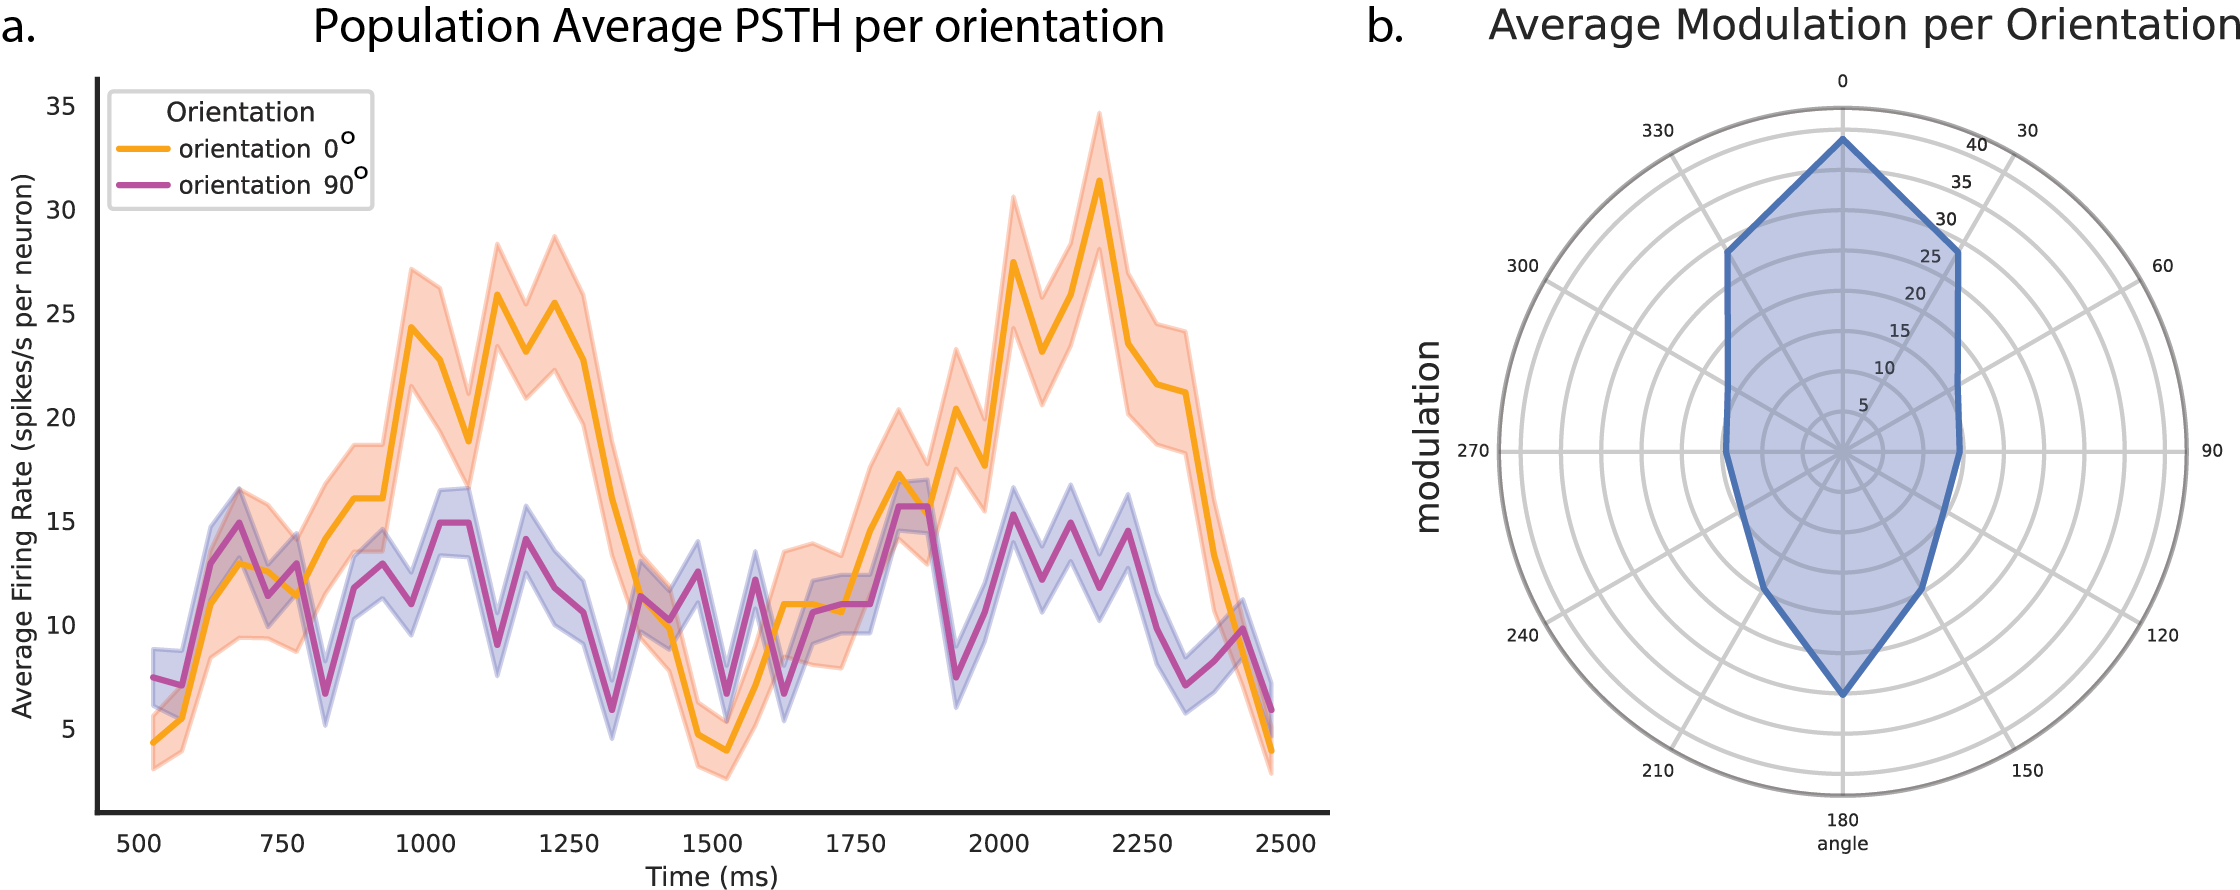
\includegraphics[width=1.0 \textwidth]{figures/figure_simple_orientation_tuning.png}
    \caption{Orientation tuning of simple V1 cells. a. The average orientation tuning of a population of simple cells. The input was a drifting grating with different orientations. In orange a horizontal drifting grating with 0 degrees orientation, and in purple a drifting grating with a 90 degree orientation. Simple cells show a phase sensitivity demonstrated by the two peaks, in which the cell receives no input from the dLGN. The polar plot shows the average firing modulation per orientation, showing that the cells respond to stimuli with both 0 and 180 degrees orientation.}
    \label{fig:simple cell orientation tuning}
\end{figure}

%\subsection{Polarity Invariance of Complex Cells.}
Complex cells are characterised by their ability to respond to edges in their receptive field regardless of input polarity. To achieve this, we connected simple cells that respond to different phases of a retinotopic coordinate. We selected five ON/OFF and five OFF/ON simple cells with similar orientation preferences, resulting in overlapping ON and OFF fields. This overlap created a receptive field that responds to both ON and OFF feedforward inputs. The connection rule for connecting simple cells to complex cells was similar to that used for connecting dLGN cells to simple cells. It iterated over all possible simple cell sources to determine if they fell within the elliptical receptive field of the target complex cell. Because the simple cell sources had similar orientation selectivity, the resulting complex cell also followed this orientation preference.

To test whether our complex cells demonstrated polarity and phase invariance, we presented the circuit with a drifting grating in the preferred orientation of the complex cell \hyperref[fig:polarity invariance]{(figure 7b)}. The drifting grating induced an alternating pattern between white and black in one spot of the visual field. Consequently, ON/OFF cells and OFF/ON cells showed alternating peaks in activity, while complex cells maintained a stable firing pattern. In figure \hyperref[fig:polarity invariance]{(figure 7a)}, the simple cell types clearly showed peaks at 30 Hz, decreasing to 0 Hz. In contrast, due to the converging simple cells, the complex cells exhibited stable activity above 30 Hz, as highlighted in the raster plots \hyperref[fig:polarity invariance]{(figure 7c)}. With these fundamental cell types and the addition of inhibitory interneurons, it is possible to create endstopped length-tuned cells.


% Subsequently, complex cells were created by selectively connecting these simple cells with each other. The process began by combining simple cells responsive to different phases, ON/OFF and OFF/ON, to form complex cells; with the goal of creating a phase invariant complex cell. 

% To create complex cells that respond to contours within their receptive field regardless of input polarity, 5 to 10 retinotopically aligned simple cells were connected to achieve overlapping ON/OFF and OFF/ON receptive fields. The converging simple cells all had the same preferred orientation but different spatial phases creating a single complex cell \hyperref[fig:LIF_Overview]{(Figure 4b)}. 

% The connection rule was used similar to that of the simple cells, which iterated over all possible simple cell sources for each target complex cell, checking for alignment in orientation and differences in phase. Synaptic connections were established between the simple cells and the complex cell, ensuring that the complex cell received inputs from a diverse set of simple cells. This convergence allowed the complex cell to respond to a range of spatial phases of a given orientation, thereby achieving polarity invariance. To test whether our complex cells demonstrated polarity and phase invariance we presented the circuit with a drifting grating in the preferred orientation of the complex cell \hyperref[fig:polarity invariance]{figure 7 b}. The drifting grating would in one spot of the visual field induce an alternating pattern between white and black. Therefore, ON/OFF cells and OFF/ON cells would also show an alternating peak in activity, whereas complex cells are expected to have a more stable firing pattern. In figure 6a the simple cell types clearly showed peaks at 30 Hz and decreasing to 0 Hz. In contrast, due to the converging simple cells, the complex cells have a stable activity above 30 Hz, also highlighted in the raster plots \hyperref[fig:polarity invariance]{figure 7c}. With these fundamental cell types with the addition of inhibitory interneurons it is possible to create endstopped length tuned cells. 

\begin{figure}[H]
    \centering
    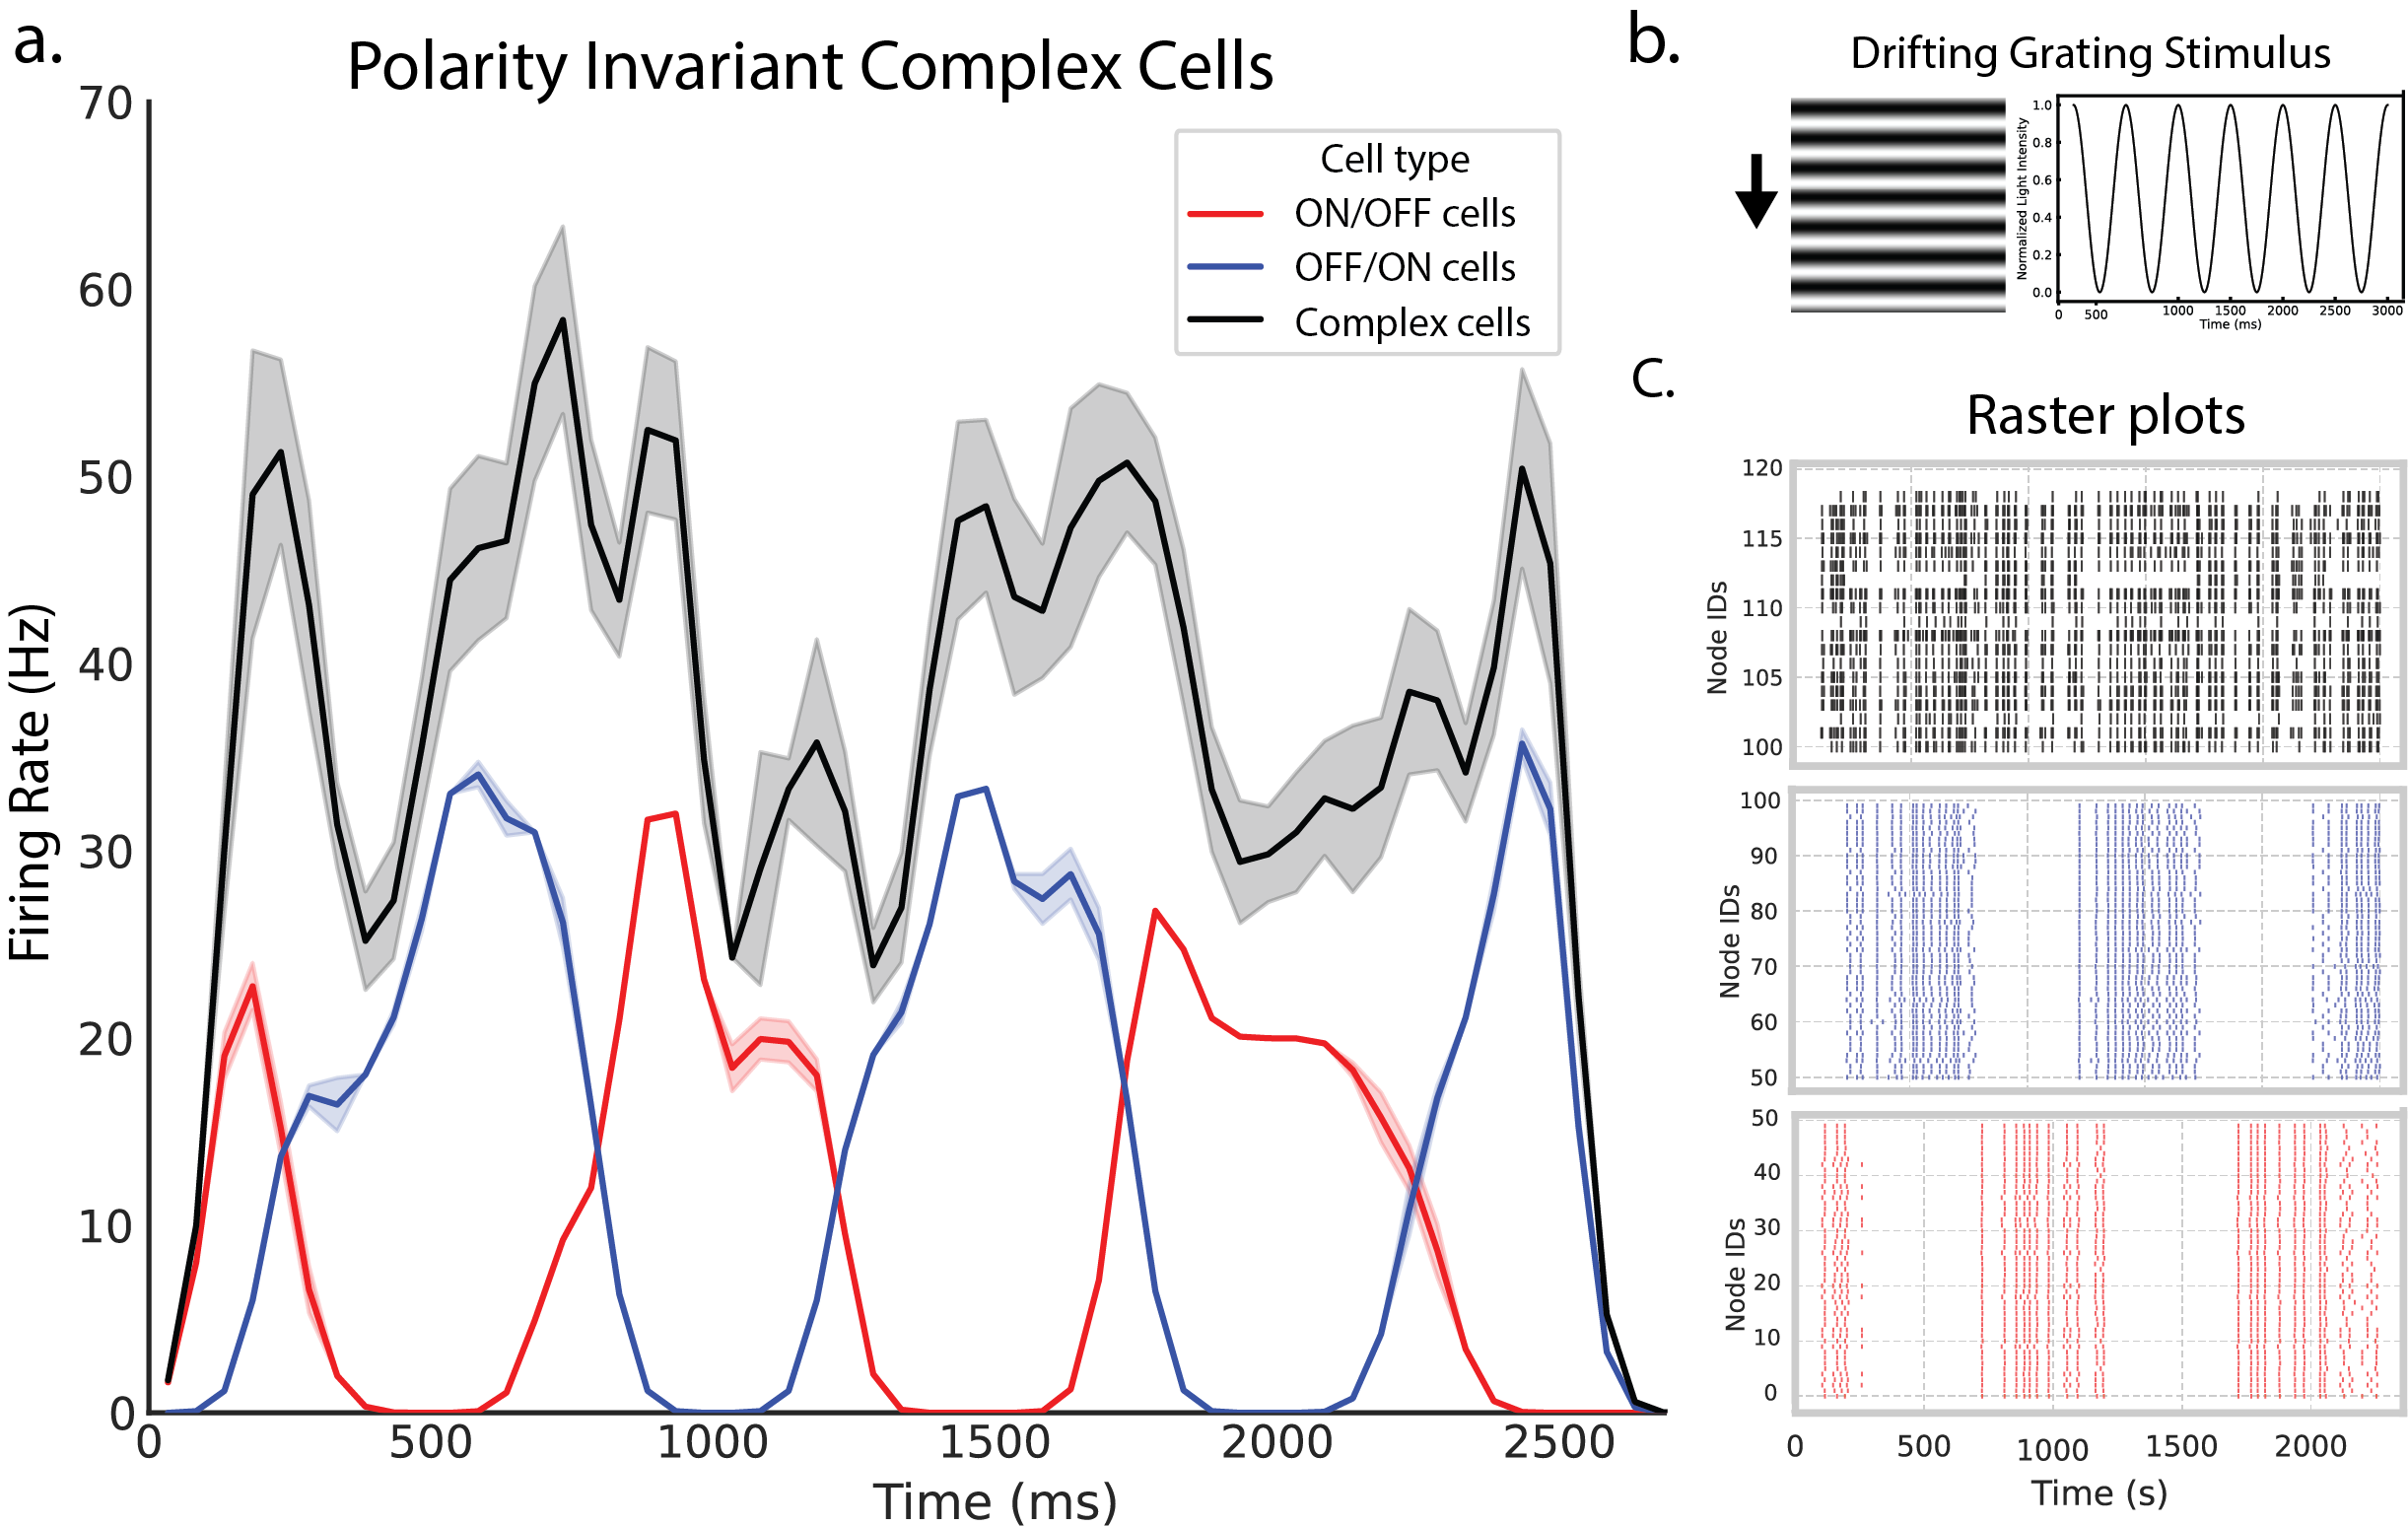
\includegraphics[width=1 \textwidth]{figures/complex_invariance_figure.png}
    \caption{Simple and complex cells responses to a horizontal drifting grating. a. ON/OFF simple cells are shown in red with an offset phase from the OFF/ON cells. The black complex cells do not exhibit the same phase sensitivity but have a more stable response to the ON and OFF alternating stimulus contrast. b. The drifting grating stimulus that was presented to the model. The orientation of the drifting grating matched the preferred orientation of all cell types. c. The raster plots also illustrate the phase sensitivity of the simple cells and how the complex cell has a stable firing to a constantly fluctuating input.}
    \label{fig:polarity invariance}
\end{figure}

%\subsection{Recurrent feedback underlying endstopping.}
Currently, only dLGN, simple cells, and complex cells were described. One goal of the model was to experiment with generating stable endstopping using these cell types. Initially, an attempt was made to create endstopping by combining spatially offset simple cells in a strictly excitatory manner, modelling the inhibitory subfield with an OFF field and the excitatory subfield with an ON field. While this method reduced the firing rate, it did not achieve a zero spiking rate for long inputs due to the excitatory nature, which could only lose half the input based on polarity. To address this, we decided to include a recurrent inhibitory loop from a laterally displaced complex cell to a neighbouring simple cell population. The displacement introduced a spatial offset between the excitation source and the inhibitory location. Resulting in a feedback loop that suppresses cell activity when a stimulus extended beyond their receptive field, the main characteristic of an endstopped cell. Because the inhibitory cells are targeted by a complex cell, the decrease in firing rate is contrast insensitive \hyperref[fig:LIF_connectivity]{(figure 4c)}. The weights that were used to connect each cell type are presented in table 3.  

% Currently, only dLGN, simple cells, and complex cell were described. One of the goals of the model was to experiment with different ways of generating stable endstopping using these cell types. In the initial phases of the LIF model an attempt was made to create endstopping by combining spatially offset simple cells to create endstoping in a strictly excitatory manner. The idea was to converge specific simple ON and OFF fields relative to each other, modelling the inhibitory subfield of an endstopped cell with an OFF field and the excitatory subfield with an ON field. While this method reduced the firing rate, it did not achieve a zero spiking rate for long inputs. The main problem was that due to the excitatory nature you could only lose maximally half the input based on polarity. To remedy this and create endstopped cells that could be inhibited to complete silence, in subsequent methods, we first integrated the simple ON/OFF streams into complex cells before introducing spatial relationships between cells. And then, to create orientation-selective and phase-invariant cells that exhibit endstopping behaviour, we used recurrent activation of inhibitory cells to model endstopping. The next step involved a laterally displaced complex cell. This neighbouring complex cell then projected to a population of inhibitory interneurons that was connected to the original simple cell population \hyperref[fig:LIF_Overview]{figure 4c}. This displacement was crucial as it introduced a spatial offset between the excitation source and the location where inhibition would be applied. The inhibitory interneurons targeted by these projections played a key role in modulating the activity of the simple cells. Once activated by the complex cells, the inhibitory cells provide feedback to the simple cells positioned in the retinotopically overlapping area of the original complex cells. This feedback loop was designed to suppress the activity of the simple cells when a stimulus extended beyond their receptive field. In more detail, as a line or bar stimulus moved across the receptive field of a simple cell and extended beyond it, the laterally displaced complex cell would activate the inhibitory interneurons. These interneurons, in turn, would inhibit the simple cells, thereby reducing their firing rate. This inhibition is a hallmark of endstopping, where the neuron's response is curtailed when a stimulus exceeds the optimal length within its receptive field. The introduction of this recurrent feedback mechanism was essential for creating endstopped cells, which are specialised for detecting the endpoints of lines and bars. Endstopped cells are known for their ability to signal the presence of corners, line ends, and other salient features in the visual field, making them critical for complex shape and motion perception. By implementing this feedback loop, the model could replicate the rapid decline in firing rate that characterises endstopping, providing a more accurate and nuanced representation of visual processing as seen in the primary visual cortex. This approach highlights the importance of inhibitory feedback in fine-tuning the responses of neurons to visual stimuli, ensuring that the network could adapt to varying stimulus lengths and shapes. To investigate further how endstopped cells can be effectively integrated with higher visual areas, the same neural architecture can be used with neural populations instead of individual LIF cells. 

%ToDo change exc inh etc. to population names
\begin{table}[h]
  \centering
  \caption{Connection Weights in the LIF endstop Circuit}
  %\label{tab:weights}
  \begin{tabular}{@{}llcc@{}}
      \toprule
      \textbf{From} & \textbf{To} & \textbf{Weight} & \textbf{Delay (ms)} \\ \midrule
      dLGN (e) & Simple (e) & 0.8 & 0.2 \\
      Simple (e) & Endstopped (e) & 0.8 & 0.2 \\
      Simple (e) & Complex (e) & 0.7 & 0.2 \\
      Complex (e) & PV (i) & 2.5 & 0.2 \\
      PV (i) & Simple (e) & -3.0 & 0.2 \\ \bottomrule
  \end{tabular}
\end{table}

%\subsection{Population activity and illusory contour representation.}
To investigate how endstopped cells can be effectively integrated into higher visual areas, we used neural population models instead of LIF cells while maintaining the same neural architecture. These population models allowed us to recreate interlaminar connections by treating each functional cell type as a population, enabling us to study how they collectively encoded the presence of illusory contours. This abstraction facilitated the addition of a higher visual cortical area, LM, which integrated V1 endstopped responses and provided cell-type-specific recurrent feedback.

The cells that integrated the endstopped responses are called pattern cells, created based on the feedforward orientation selectivity of the endstopped sources. Their feedback targeted orthogonally tuned complex cells, corresponding to the orientation of the resulting illusory contour \hyperref[fig:illusory_filling]{figure 8}. This way, specific endstopped cells were active due to the horizontal inducers, without activating the inhibitory feedback loop. If enough inducers were active, those signals would be integrated and activate the LM pattern cells, resulting in an excitatory feedback loop that fills in the illusory contour between the inducers.


% The population models allowed us to recreate the interlaminar endstopping microcircuits by treating each cell type as a specific population and study how multiple endstopping microcircuits collectively encoded the presence of illusory contours in a specific retinotopic coordinate of the visual field. This way we still captured the dynamic interactions between simple, complex, endstopping, and inhibitory interneurons, while providing a network of which the activity could be further integrated in a higher visual cortical area such as LM, the second visual area in the mouse. In turn, this allowed us to examine how higher level visual feedback could provide information for V1 to induce an illusory filling in mechanism between retinotopic coordinates. Thus, abstracting the LIF model into a population model allowed for a more comprehensive view of how V1 processes visual information in the case of possible occlusion and how an illusory response can be generated to particular stimulus configurations. The final endstopped cells were generated across the grid with specified offsets to ensure coverage of the visual field, and each was assigned a position based on its offset values. Simple cells were derived from the complex cells, inheriting their properties, and inhibitory cells were created to modulate the activity of the simple and complex cells. Pattern cells were generated based on specified orientations and positions to represent orthogonal illusory lines compared to the endstopped cell input they received. Connections from pattern cells to complex and endstop cells facilitated the feedback mechanisms required for simulating illusory contours \hyperref[fig:illusory_filling]{figure 8}. Particular endstopped cells are active due to the horizontal inducers ending within their excitatory receptive field, without activating the inhibitory feedback loop driven by the complex cell. In turn if enough inducers are present those signals would be integrated in the LM pattern cell, with an excitatory feedback loop as a results, filling in the illusory contour between the inducers. Therefore, the current model simulates the generation of illusory contours, based on multiple recurrent feedback loops, one inhibitory local for endstopping and one excitatory between V1 and LM. 
%ToDo describe connectivity patterns used to create population model.


\vspace{20pt}
\begin{figure}[H]
  \centering
  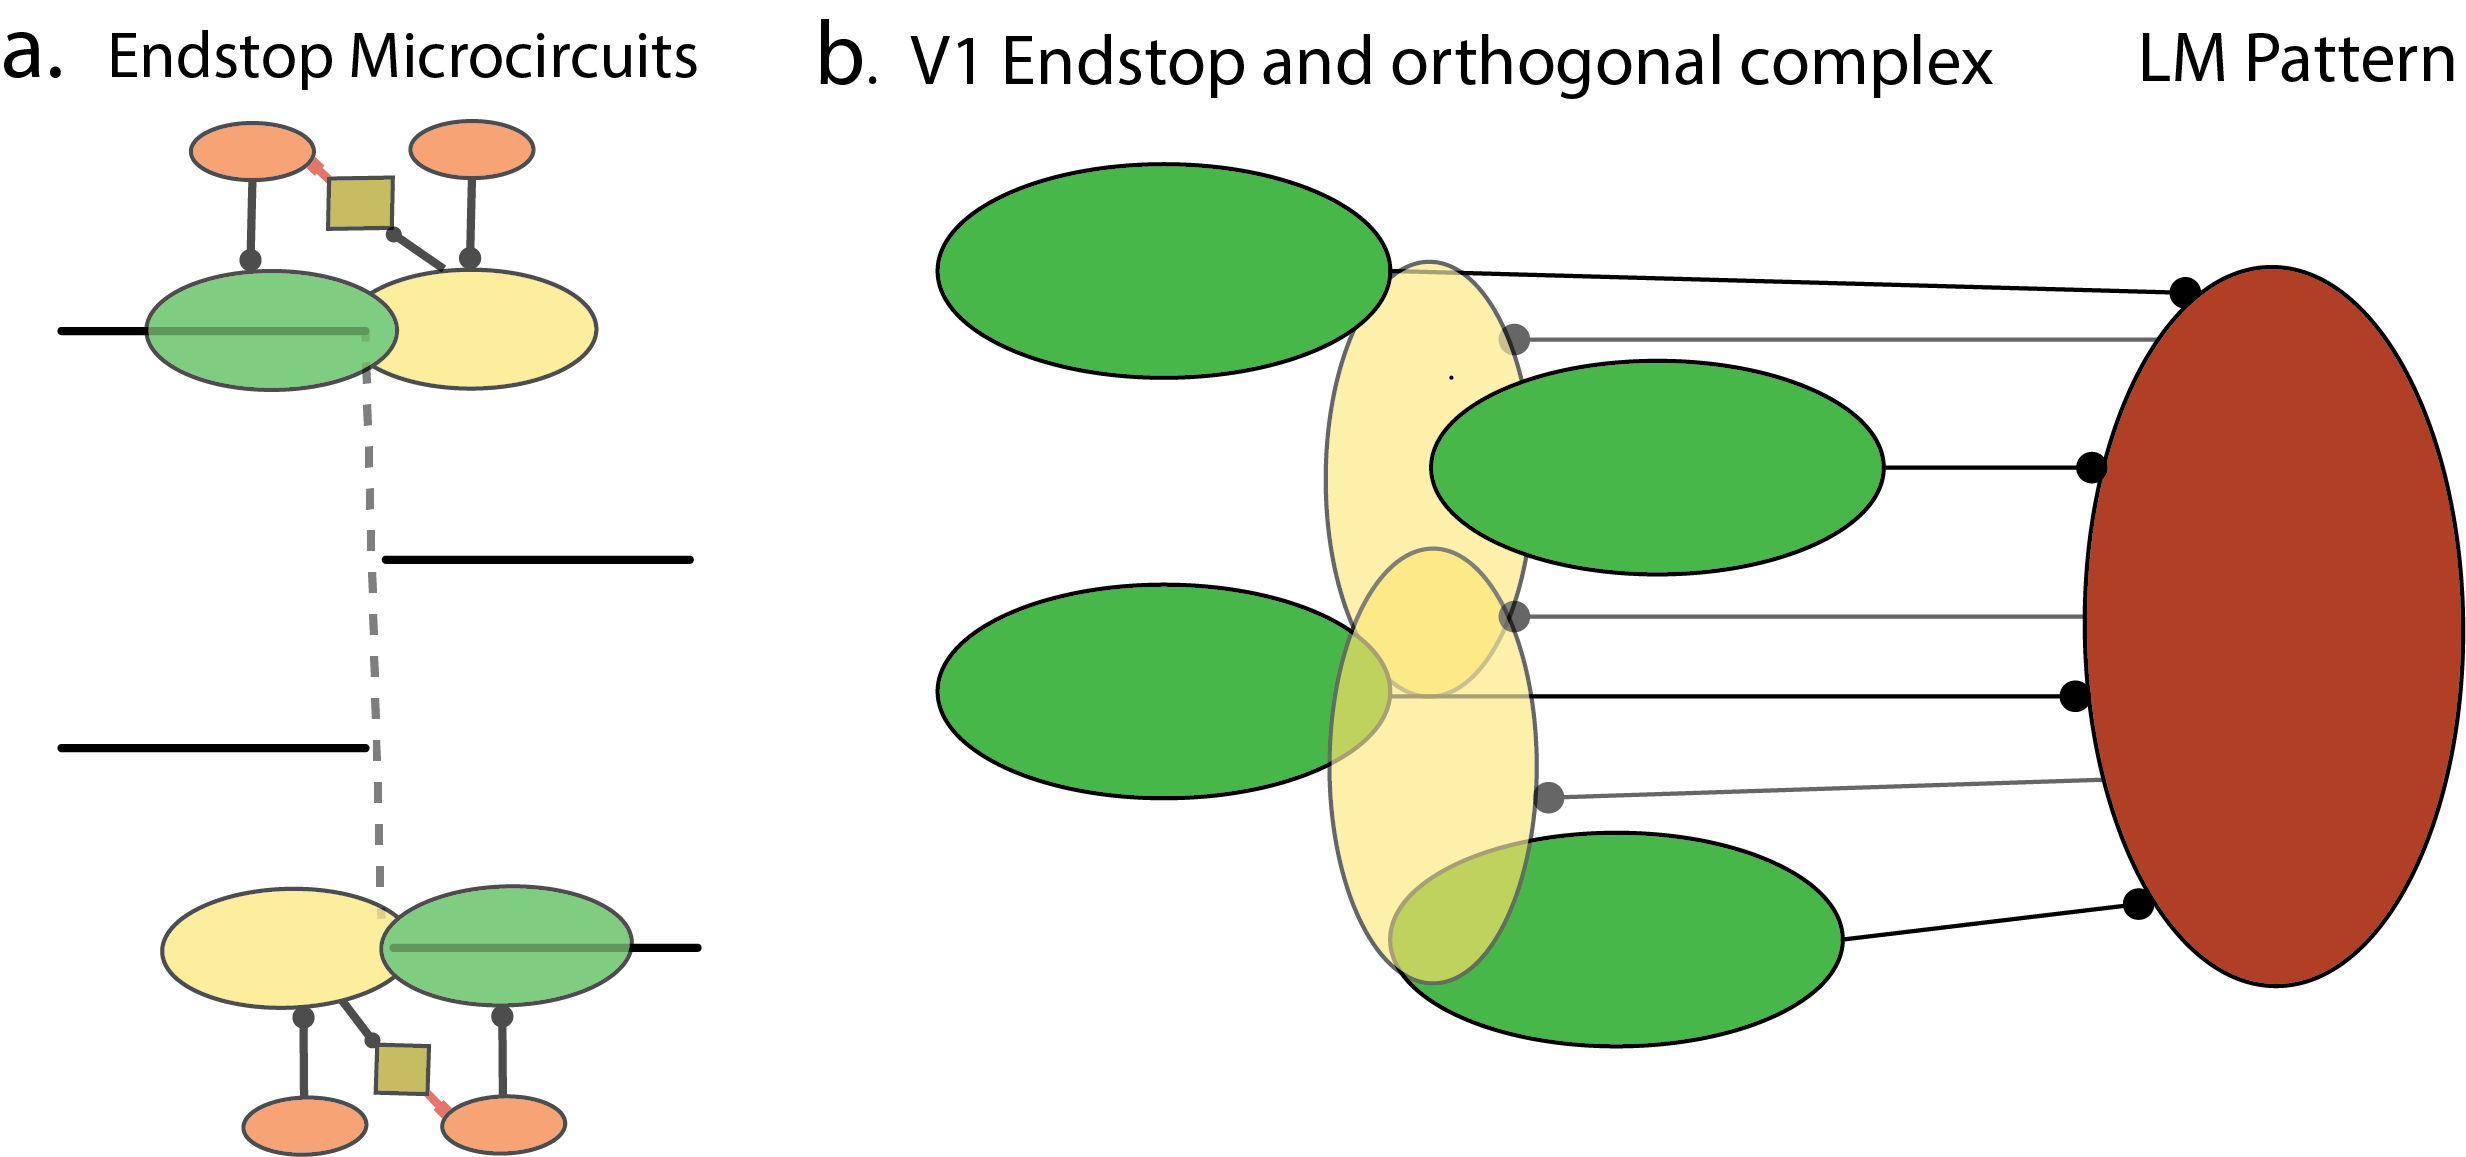
\includegraphics[width=1 \textwidth]{adjusted_figures/illusory_filling.png}
  \caption{The architecture used to represent illusion inducer objects through the feedforward endstopped signals and the representation of illusory contours through feedback responses. a. The endstopped microcircuit illustrated on top of horizontal abutting grating illusion inducers. The cells are colour coded following \hyperref[fig:LIF_Overview](figure 4). b. If all 4 of the endstopped cells are active they fire intensely enough to activate a higher visual pattern cell in LM, which integrates these input and projects feedback onto orthogonally tuned complex cells. This way an illusory contour is locally represented through the integration of local endstopped signals.}
  \label{fig:illusory_filling}
\end{figure}
\newpage
% ToDo check and rewrite
% \subsubsection{PyRates Library and population parameters.}
% The Wilson and Cowan neural mass model within the PyRates library captures the average firing rate dynamic of populations of LIF cells \autocite{wilsonExcitatoryInhibitoryInteractions1972}. The model consists of several key components and parameters that we will explain in detail.
% First, we define an operator called the synaptic excitation operator. This operator uses a sigmoid function to model the process of synaptic excitation. The equation for this operator is:
% \[
% m = \operatorname{sigmoid}(s \cdot (r_{\mathrm{in}} + r_{\mathrm{ext}} - \theta)) - \operatorname{sigmoid}(-s \cdot \theta),
% \]
% where \( m \) represents the output signal from the neuron. The term \(\operatorname{sigmoid}\) is a mathematical function that smoothly limits the output between 0 and 1, mimicking the neuron's firing rate. The parameter \( s \) controls the steepness of the sigmoid curve and is set to 1.0, meaning it defines how quickly the neuron responds to input. The parameter \(\theta\) is a threshold set to 2.0, which the input must exceed for the neuron to start firing. The inputs \( r_{\mathrm{in}} \) and \( r_{\mathrm{ext}} \) represent signals coming from other neurons and external sources, respectively, and both are initially set to 0.0.
% We also have a variation called the synaptic inhibition operator. This operator works similarly but models inhibitory signals, which reduce neuron activity. Its equation is similar, but with different parameters: \( s \) is set to 2.0, making the response steeper, and \( \theta \) is set to 2.5, meaning a higher threshold for inhibition.
% Next, we describe the rate operator. This operator models the rate of change in neural activity over time using the differential equation:
% \[
% r' = \frac{-r + (1.0 - k \cdot r) \cdot m}{\tau}.
% \]
% Here, \( r \) is the current activity level of the neuron, initially set to 0.0. The parameter \( k \) is set to 1.0 and influences how the neuron's activity decreases over time. The term \( \tau \) represents the time constant set to 10.0, which defines how quickly the neuron activity responds to changes. The input \( m \) is the signal calculated by the excitation or inhibition operators.
% To model neural populations, we use node templates. The excitatory population node template combines the rate operator and the synaptic excitation operator to represent a group of excitatory neurons, which promote activity in the network. Conversely, the inhibitory population node template combines the rate operator and the synaptic inhibition operator to represent a group of inhibitory neurons, which suppress activity in the network.

% The node templates can be combine to form a circuit template defining the grand network structure of the model. The Wilson-Cowan circuit template that was used consists of two nodes types an excitatory population and an inhibitory types, that are connected similarly to the LIF model to induce functional variation between simple, complex and endstopped cells. The parameters used in the model are summarised in Table~\ref{tab:parameters}.

%----
% The Wilson and Cowan neural mass model within the PyRates library is a phenomenological model but effectively captures the steady-states in average firing rates of excitatory and inhibitory populations of LIF neurons \autocite{wilsonExcitatoryInhibitoryInteractions1972}. The dynamics of each population are described by a first-order ordinary differential equation:

% \[
% \tau \dot{r} = -r + (k - q r) S(m),
% \]

% where \( r \) represents the average firing rate of the population, \( \tau \) is a lumped population time constant, \( k \) is a coupling term, \( q \) is a refractory term, and \( S(m) \) is the synaptic input. Typically, \( S \) is chosen as a sigmoidal transfer function that transforms the pre-synaptic membrane potential into an average firing rate:

% \[
% S(m) = \frac{1}{1 + e^{-m}}.
% \]

% For both excitatory (E) and inhibitory (I) populations, the Wilson-Cowan model is described via two coupled ODEs:

% \[
% \begin{aligned}
% \tau_e \dot{r}_e &= -r_e + (k_e - q_e r_e) S(c_{ee} r_e + c_{ei} r_i + I_e(t)), \\
% \tau_i \dot{r}_i &= -r_i + (k_i - q_i r_i) S(c_{ie} r_e + c_{ii} r_i + I_i(t)),
% \end{aligned}
% \]

% where \( r_e \) and \( r_i \) represent the firing rates of excitatory and inhibitory populations, respectively. The parameters \( \tau_e \) and \( \tau_i \) are the time constants, \( k_e \) and \( k_i \) are coupling terms, and \( q_e \) and \( q_i \) are refractory terms for excitatory and inhibitory populations, respectively. The terms \( c_{ee} \), \( c_{ei} \), \( c_{ie} \), and \( c_{ii} \) represent the connection weights between populations, and \( I_e(t) \) and \( I_i(t) \) are additional extrinsic inputs. The node templates can be combine to form a circuit template defining the grand network structure of the model. The Wilson-Cowan circuit template that was used consists of two nodes types an excitatory population and an inhibitory population, that are connected similarly to the LIF model to induce functional variation between simple, complex and endstopped cells. The parameters used in the model are summarised in Table~\ref{tab:parameters}.
%---
% The Wilson-Cowan neural mass model within the PyRates library is a phenomenological model that effectively captures the steady-states in average firing rates of excitatory and inhibitory populations of LIF neurons \autocite{wilsonExcitatoryInhibitoryInteractions1972}. The dynamics of each population are described by a first-order ordinary differential equation:

% \[
% \tau \dot{r} = -r + (k - q r) S(m),
% \]

% where \( r \) represents the average firing rate of the population, \( \tau \) is a population time constant, \( k \) is a coupling term, \( q \) is a refractory term, and \( S(m) \) is the synaptic input. Typically, \( S \) is chosen as a sigmoidal transfer function that transforms the pre-synaptic membrane potential into an average firing rate:

% \[
% S(m) = \frac{1}{1 + e^{-m}}.
% \]

% For both excitatory (E) and inhibitory (I) populations, the Wilson-Cowan model is described via two coupled ODEs:

% \[
% \begin{aligned}
% \tau_e \dot{r}_e &= -r_e + (k_e - q_e r_e) S(c_{ee} r_e + c_{ei} r_i + I_e(t)), \\
% \tau_i \dot{r}_i &= -r_i + (k_i - q_i r_i) S(c_{ie} r_e + c_{ii} r_i + I_i(t)),
% \end{aligned}
% \]

% where \( r_e \) and \( r_i \) represent the firing rates of excitatory and inhibitory populations, respectively. The parameters \( \tau_e \) and \( \tau_i \) are the time constants, \( k_e \) and \( k_i \) are coupling terms, and \( q_e \) and \( q_i \) are refractory terms for excitatory and inhibitory populations, respectively. The terms \( c_{ee} \), \( c_{ei} \), \( c_{ie} \), and \( c_{ii} \) represent the connection weights between populations, and \( I_e(t) \) and \( I_i(t) \) are additional extrinsic inputs.

% The synaptic excitation operator uses a sigmoid function to model the process of synaptic excitation. The equation for this operator is:

% \[
% m = \operatorname{sigmoid}(s \cdot (r_{\mathrm{in}} + r_{\mathrm{ext}} - \theta)) - \operatorname{sigmoid}(-s \cdot \theta),
% \]

% where \( m \) represents the output signal from the neuron. The \(\operatorname{sigmoid}\) function is defined as:

% \[
% \operatorname{sigmoid}(m) = \frac{1}{1 + e^{-m}}.
% \]

% Here, \( s \) controls the steepness of the sigmoid curve and is set to 1.0, defining how quickly the neuron responds to input. The parameter \(\theta\) is a threshold set to 2.0, which the input must exceed for the neuron to start firing significantly. The terms \( r_{\mathrm{in}} \) and \( r_{\mathrm{ext}} \) represent internal and external inputs to the neuron, respectively, where \( r_{\mathrm{in}} \) is the input from other neurons within the same network and \( r_{\mathrm{ext}} \) is input from external sources.

% The synaptic inhibition operator works similarly but models inhibitory signals that reduce neuron activity. Its equation is similar, but with different parameters: \( s \) is set to 2.0, making the response steeper, and \(\theta\) is set to 2.5, indicating a higher threshold for inhibition.

% The rate operator models the rate of change in neural activity over time using the differential equation:

% \[
% \tau \dot{r} = -r + (k - q \cdot r) S(m),
% \]

% where \( r \) is the current activity level of the neuron. The parameter \(\tau\) is the time constant set to 10.0, \( k \) is a coupling term set to 1.0, and \( q \) is a refractory term. The input \( m \) is the signal calculated by the excitation or inhibition operators.

% To model neural populations, we use node templates. The excitatory population node template combines the rate operator and the synaptic excitation operator to represent a group of excitatory neurons, which promote activity in the network. Conversely, the inhibitory population node template combines the rate operator and the synaptic inhibition operator to represent a group of inhibitory neurons, which suppress activity in the network. These node templates can be combined to form a circuit template defining the grand network structure of the model. The Wilson-Cowan circuit template used consists of two node types: an excitatory population and an inhibitory population, connected similarly to the LIF model to induce functional variation between simple, complex, and end-stopped cells. The parameters used in the model are summarised in Table~\ref{tab:parameters}.

% \begin{table}[h]
%     \centering
%     \caption{Parameters of the Wilson-Cowan Neural Mass Model}
%     \label{tab:parameters}
%     \begin{tabular}{@{}lll@{}}
%         \toprule
%         \textbf{Parameter} & \textbf{Description} & \textbf{Value} \\ \midrule
%         \( s \) & Steepness of the sigmoid curve (excitation) & 1.0 \\
%         \( \theta \) & Threshold for excitation & 2.0 \\
%         \( r_{\mathrm{in}} \) & Input from other neurons & 5.0 \\
%         \( r_{\mathrm{ext}} \) & External input & 0.0 \\
%         \( s \) (inhibition) & Steepness of the sigmoid curve & 2.0 \\
%         \( \theta \) (inhibition) & Threshold for inhibition & 2.5 \\
%         \( r \) & Current activity level & 0.0 \\
%         \( k \) & Decay parameter for activity & 1.0 \\
%         \( \tau \) & Time constant (ms) & 10.0 \\ \bottomrule
%     \end{tabular}
% \end{table}
%ToDo: their are 2 times the sigmoidal function in here need to change this
% The Wilson-Cowan neural mass model within the PyRates library is a phenomenological model that effectively captures the steady-states in average firing rates of excitatory and inhibitory populations of LIF neurons \autocite{wilsonExcitatoryInhibitoryInteractions1972}. The dynamics of each population are described by a first-order ordinary differential equation (ODE):

% \[
% \tau \dot{r} = -r + (k - q r) S(m),
% \]

% where \( r \) represents the average firing rate of the population, \( \tau \) is a population time constant, \( k \) is a coupling term, \( q \) is a refractory term, and \( S(m) \) is the synaptic input. \( S \) is chosen as a sigmoidal transfer function that transforms the pre-synaptic membrane potential into an average firing rate:

% \[
% S(m) = \frac{1}{1 + e^{-m}}.
% \]
% where \( m \) represents the output signal from the neuron. The \(\operatorname{sigmoid}\) function is defined as:
% \[
% m = \operatorname{sigmoid}(s \cdot (r_{\mathrm{in}} + r_{\mathrm{ext}} - \theta)) - \operatorname{sigmoid}(-s \cdot \theta),
% \]

% Here, \( s \) controls the steepness of the sigmoid curve and is set to 1.0, defining how quickly the neuron responds to input. The parameter \(\theta\) is a threshold set to 2.0, which the input must exceed for the neuron to start firing significantly. The terms \( r_{\mathrm{in}} \) and \( r_{\mathrm{ext}} \) represent inhibitory and excitatory states of the population, respectively, where \( r_{\mathrm{in}} \). The balance between the inhibitory and excitatory population activatiy determines the net effect of incoming inputs.

% For both excitatory (E) and inhibitory (I) populations, the Wilson-Cowan model is described via two coupled ODEs:

% \[
% \begin{aligned}
% \tau_e \dot{r}_e &= -r_e + (k_e - q_e r_e) S(c_{ee} r_e + c_{ei} r_i + I_e(t)), \\
% \tau_i \dot{r}_i &= -r_i + (k_i - q_i r_i) S(c_{ie} r_e + c_{ii} r_i + I_i(t)),
% \end{aligned}
% \]

% where \( r_e \) and \( r_i \) represent the firing rates of excitatory and inhibitory populations, respectively. The parameters \( \tau_e \) and \( \tau_i \) are the time constants, \( k_e \) and \( k_i \) are coupling terms, and \( q_e \) and \( q_i \) are refractory terms for excitatory and inhibitory populations, respectively. The terms \( c_{ee} \), \( c_{ei} \), \( c_{ie} \), and \( c_{ii} \) represent the connection weights between populations, and \( I_e(t) \) and \( I_i(t) \) are additional extrinsic inputs.

% % The synaptic excitation operator uses a sigmoid function to model the process of synaptic excitation. The equation for this operator is:





% % \[
% % \operatorname{sigmoid}(m) = \frac{1}{1 + e^{-m}}.
% % \]



% The synaptic inhibition operator works similarly but models inhibitory signals that reduce neuron activity. Its equation is similar, but with different parameters: \( s \) is set to 2.0, making the response steeper, and \(\theta\) is set to 2.5, indicating a higher threshold for inhibition.

% To model neural populations, we use node templates. The excitatory population node template combines the rate operator and the synaptic excitation operator to represent a group of excitatory neurons, which promote activity in the network. Conversely, the inhibitory population node template combines the rate operator and the synaptic inhibition operator to represent a group of inhibitory neurons, which suppress activity in the network. These node templates can be combined to form a circuit template defining the grand network structure of the model. The Wilson-Cowan circuit template used consists of two node types: an excitatory population and an inhibitory population, connected similarly to the LIF model to induce functional variation between simple, complex, and end-stopped cells. The parameters used in the model are summarised in Table~\ref{tab:parameters}.


%--new
% The Wilson-Cowan model describes the dynamics of excitatory and inhibitory neural populations through coupled differential equations. The rate equations for the excitatory and inhibitory populations are given by:

% \[
% \begin{aligned}
% \tau_e \dot{r}_e &= -r_e + (k_e - q_e r_e) S(c_{ee} r_e + c_{ei} r_i + I_e(t)), \\
% \tau_i \dot{r}_i &= -r_i + (k_i - q_i r_i) S(c_{ie} r_e + c_{ii} r_i + I_i(t)),
% \end{aligned}
% \]

% where \( \tau_e \) and \( \tau_i \) are time constants for the excitatory and inhibitory populations, respectively, and \( r_e \) and \( r_i \) are the firing rates of these populations. The constants \( k_e \), \( k_i \), \( q_e \), and \( q_i \) relate to the maximum firing rates and their saturation. The coupling coefficients \( c_{ee} \), \( c_{ei} \), \( c_{ie} \), and \( c_{ii} \) represent the connection strengths between the populations, while \( I_e(t) \) and \( I_i(t) \) are the external inputs to the excitatory and inhibitory populations, respectively.

% The sigmoid function \( S \), which transforms the combined synaptic inputs into a firing rate, is given by:

% \[
% \text{sigmoid}(x) = \frac{1}{1 + e^{-x}}
% \]

% In the context of the Wilson-Cowan model, the sigmoid operation is expressed as:

% \[
% m = \text{sigmoid}(s \cdot (r_{\text{in}} + r_{\text{ext}} - \theta)) - \text{sigmoid}(-s \cdot \theta)
% \]

% Here, \( r_{\text{in}} \) represents the intrinsic input from within the network, such as \( c_{ee} r_e \) or \( c_{ii} r_i \), and \( r_{\text{ext}} \) represents extrinsic inputs like \( I_e(t) \) or \( I_i(t) \). The parameters \( s \) and \( \theta \) control the slope and threshold of the sigmoid function, respectively. The sigmoid function normalises the input, producing an output firing rate \( m \) that captures the balance between excitatory and inhibitory inputs. This transformed firing rate is then used in the rate equations to describe the dynamic behaviour of the neural populations.

% %--

% \begin{table}[h]
%   \centering
%   \caption{Parameters of the Wilson-Cowan Neural Mass Model}
%   \label{tab:parameters}
%   \begin{tabular}{@{}lll@{}}
%       \toprule
%       \textbf{Parameter} & \textbf{Description} & \textbf{Value} \\ \midrule
%       \( s \) & Steepness of the sigmoid curve (excitation) & 1.0 \\
%       \( \theta \) & Threshold for excitation & 2.0 \\
%       \( r_{\mathrm{in}} \) & Inhibitory state of the population & 0.0 \\
%       \( r_{\mathrm{ext}} \) & Excitatory state of the population & 0.0 \\
%       \( s \) (inhibition) & Steepness of the sigmoid curve & 2.0 \\
%       \( \theta \) (inhibition) & Threshold for inhibition & 2.5 \\
%       \( r \) & Initial activity level & 0.0 \\
%       \( k \) & Decay parameter for activity & 2.0 \\
%       \( \tau \) & Time constant (ms) & 10.0 \\ \bottomrule
%   \end{tabular}
% \end{table}

%-- newest extended:
The population mass model we used was the Wilson and Cowan model \autocite{wilsonExcitatoryInhibitoryInteractions1972}. The model describes the dynamics of excitatory and inhibitory neural populations through coupled differential equations. The rate equations for the excitatory and inhibitory populations are given by:

\[
\begin{aligned}
\tau_e \dot{r}_e &= -r_e + (k_e - q_e r_e) S(c_{ee} r_e + c_{ei} r_i + I_e(t)), \\
\tau_i \dot{r}_i &= -r_i + (k_i - q_i r_i) S(c_{ie} r_e + c_{ii} r_i + I_i(t)),
\end{aligned}
\]

where \( \tau_e \) and \( \tau_i \) are time constants for the excitatory and inhibitory populations, respectively, and \( r_e \) and \( r_i \) are the firing rates of these populations. The constants \( k_e \), \( k_i \), \( q_e \), and \( q_i \) relate to the maximum firing rates and their saturation. The coupling coefficients \( c_{ee} \), \( c_{ei} \), \( c_{ie} \), and \( c_{ii} \) represent the connection strengths between the populations, while \( I_e(t) \) and \( I_i(t) \) are the external inputs to the excitatory and inhibitory populations, respectively.

The sigmoid function \( S \), which transforms the combined synaptic inputs into a firing rate, is given by:

\[
\text{sigmoid}(x) = \frac{1}{1 + e^{-x}}
\]

In the context of the Wilson-Cowan model, the sigmoid operation is expressed as:

\[
m = \text{sigmoid}(s \cdot (r_{\text{exc}} + r_{\text{inh}} - \theta)) - \text{sigmoid}(-s \cdot \theta)
\]

Here, \( r_{\text{inh}} \) represents the inhibitory input, such as \( c_{ii} r_i \), and \( r_{\text{exc}} \) represents excitatory inputs like \( c_{ee} r_e \) or \( I_e(t) \). The parameters \( s \) and \( \theta \) control the slope and threshold of the sigmoid function, respectively. The sigmoid function normalises the input, producing an output firing rate \( m \) that captures the balance between excitatory and inhibitory inputs. This transformed firing rate is then used in the rate equations to describe the dynamic behaviour of the neural populations.

The range of the firing rate \( r \) is determined by the steady-state solutions of the rate equations. Given the typical parameters and the properties of the sigmoid function, which ranges between 0 and 1, the firing rate \( r \) will also range between 0 and a maximum value that depends on the specific parameters of the model. For the given parameter values (see Table~\ref{tab:parameters}), the firing rate \( r \) is expected to range approximately from 0 to 0.5. The model output is then multiplied by 10 to represent the firing rate in spikes per second, resulting in a range from 0 to 5 spikes per second. This range captures the steady-state behaviour under typical neural conditions and the balance of excitatory and inhibitory inputs.

To model neural populations, we use node templates. The excitatory population node template combines the rate operator and the synaptic excitation operator to represent a group of excitatory neurons, which promote activity in the network. Conversely, the inhibitory population node template combines the rate operator and the synaptic inhibition operator to represent a group of inhibitory neurons, which suppress activity in the network. These node templates can be combined to form a circuit template defining the overall network structure of the model. The parameters used in the model are summarised in Table~\ref{tab:parameters}.

\begin{table}[h]
  \centering
  \caption{Parameters of the Wilson-Cowan Neural Mass Model}
  \label{tab:parameters}
  \begin{tabular}{@{}lll@{}}
      \toprule
      \textbf{Parameter} & \textbf{Description} & \textbf{Value} \\ \midrule
      \( s \) & Steepness of the sigmoid curve (excitation) & 1.0 \\
      \( \theta \) & Threshold for excitation & 2.0 \\
      \( r_{\mathrm{inh}} \) & Inhibitory state of the population & 0.0 \\
      \( r_{\mathrm{exc}} \) & Excitatory state of the population & 0.0 \\
      \( s \) (inhibition) & Steepness of the sigmoid curve (inhibition) & 2.0 \\
      \( \theta \) (inhibition) & Threshold for inhibition & 2.5 \\
      \( k \) & Coupling term & 1.0 \\
      \( \tau \) & Time constant (ms) & 10.0 \\ \bottomrule
  \end{tabular}
\end{table}

The connections between these nodes are specified with weights that determine the strength and type of influence they exert on each other. The weights for these connections are as follows: the rate output \( r \) of the Simple (e) node feeds into the synaptic excitation input \( r_{\mathrm{exc}} \) of the Endstop (e) node with a weight of 7.0, the rate output \( r \) of the Simple (e) node also feeds into the synaptic excitation input \( r_{\mathrm{exc}} \) of the Complex (e) node with a weight of 7.0, the rate output \( r \) of the Complex node influences the PV (i) node's synaptic inhibition input \( r_{\mathrm{inh}} \) with a weight of 7.0, the rate output \( r \) of the PV (i) node reduces activity in the Simple (e) node by feeding into its synaptic excitation input \( r_{\mathrm{exc}} \) with a weight of -14.0, and the rate output \( r \) of the Pattern (e) node feeds into the synaptic excitation input \( r_{\mathrm{exc}} \) of the Complex (e) node with a weight of 12.0. The specifications of these weights are outlined in Table~\ref{tab:weights}.

\begin{table}[h]
  \centering
  \caption{Connection Weights in the Wilson-Cowan Circuit}
  \label{tab:weights}
  \begin{tabular}{@{}llc@{}}
      \toprule
      \textbf{From} & \textbf{To} & \textbf{Weight} \\ \midrule
      Simple (e) & Endstop (e) & 7.0 \\
      Simple (e) & Complex (e) & 7.0 \\
      Complex & PV (i) & 7.0 \\
      PV (i) & Simple (e) & -14.0 \\
      Pattern (e) & Complex (e) & 12.0 \\ \bottomrule
  \end{tabular}
\end{table}

\subsection*{Data analysis}
All data analyses and visualisations were performed using the Python programming language \autocite{vanrossumPythonTutorial1995}. First, spiking data was structured with a spike timestamp and a cell identification number. To track the specific cell types each cell also had a complexity identification number, corresponding to simple, complex or endstopped cells. This way each cell could be identified post simulation. Importantly, spiking behaviour was not influenced by a cell's identification number, but a product of their connectivity. The identification number only served as a way to retrieve the spikes of a particular set of cells. To visualise and analyse the spike trains over time, peristimulus time histograms (PSTH) were used. To create the PSTH, elicited spikes were counted over multiple cells per time bin (50 ms). In order to quantify the firing rate as a temporal average, the firing rate ($\nu_c$) in cell $c$ is the spike count ($n_{sp}^c$) in an interval of duration $T$ divided by $T$.

\[
V_c = \frac{nsp_c}{T}
\]

To visualise the average response of multiple neurons the cells were averaged per time bin. The resulting signal was then smoothed by convoluting the averaged PSTH with a Gaussian kernel to make trends in the data more pronounced. Additionally, the y-axis limits were fixed based on the largest response in the test.

In order to preserve single cell dynamics, the PSTH of the evoked responses of individual cells were used to calculate the modulation and endstopping accuracy. The modulation is defined as the difference between the maximum and minimum non-zero firing rates. 

\[
\text{Modulation} = \max(\text{FR}_{\text{non-zero}}) - \min(\text{FR}_{\text{non-zero}})
\]

Where \(\text{FR}_{\text{non-zero}}\) represents the non-zero firing rates.

To calculate the Signal-to-Noise Ratio (SNR), we convert the PSTH data to firing rates (in Hz) and smooth the data using a Gaussian filter. We then fit a quadratic polynomial to the smoothed firing rate data within a specified analysis window. The SNR is quantified by calculating the penalised R-squared value, which accounts for any firing rates that exceed a threshold after a specified penalty time. The formula for the penalised R-squared value is:

\[
R^2_{\text{penalised}} = \left( 1 - \frac{SS_{\text{res}}}{SS_{\text{tot}}} \right) \times P
\]

Where \(SS_{\text{res}}\) is the residual sum of squares, \(SS_{\text{tot}}\) is the total sum of squares, and \(P\) is a penalty factor that reduces the R-squared value if the firing rate exceeds a 20 Hz after the endstopped time window. We conducted an analysis to compare the endstopped accuracy measurements across the different network configurations. To assess the normality of the SNR value distributions, we employed the Kolmogorov-Smirnov (K-S) test and generated quantile-quantile (Q-Q) plots. Given that the SNR values did not follow a normal distribution, we used the Mann-Whitney U test for pairwise comparisons between the networks. This non-parametric test is suitable for comparing distributions of two independent samples with unequal sample sizes. Pairwise Mann-Whitney U tests were conducted for all combinations of network configurations, calculating the test statistic and p-value for each comparison, results were adjusted for multiple comparison using the false discovery rate (FDR) with an alpha of 0.05.
 
\section*{Results}
%\subsection{LIF Endstopped Receptive Field properties.}
\setlength{\parindent}{24pt}
To investigate the role of recurrent inhibition in the process of endstopping, we developed a LIF point neuron model comprising a microcircuit of simple, complex, and inhibitory interneurons. The simple cell population at a specified retinotopic coordinate connects to a complex cell, creating an inhibitory feedback loop that suppresses the activity of a neighbouring simple cell population. This configuration allows us to simulate the behaviour of endstopped cells in response to line segments of varying lengths and orientations. The results, as illustrated in figure \ref{fig:endstopping}, demonstrate that the endstopped cell spikes maximally when a line is positioned over the classical receptive field. However, this activity is inhibited when the line extends into the receptive field of an adjacent complex cell, due to the inhibition from the recurrent inhibitory population.
\setlength{\parindent}{0pt}
\\
\hyperref[fig:endstopping]{Figure 9} illustrates the endstopping responses within the microcircuit. The four subplots (a, b, c, d) represent the average firing rates of neurons exposed to bars of varying lengths (10, 15, 25, and 35 visual degrees) at four different orientations: 0°, 15°, 30°, and 45°. At 0° orientation, the firing rates exhibit a distinct pattern. The short bar of 20 visual degrees elicits the highest response, with firing rates peaking around 70 Hz between 100 and 200 ms after stimulus presentation and showing a significant sustained response beyond 1000 ms of the simulation. As the bar length increases, the firing rates decrease, indicating a strong endstopping effect. Bars of 15, 25, and 35 visual degrees show progressively lower peak firing rates and shorter durations of sustained activity, with the 35-degree bar almost not eliciting any response. Moreover, as the orientation of the presented bar increases, we observed a gradual decline in the initial firing rate as well as a balanced endstopping effect due to varying amounts of coverage of the complex receptive field when the bar is rotated. At a 15° orientation, the response pattern shifts slightly. The 15 visual degree bar still evokes the highest firing rate, but the peak is slightly lower than for 0° orientation, at around 50 Hz. Moreover, the relative difference between the response elicited between the 10 and 15 visual degrees is smaller compared to the horizontally oriented bar at 0° orientation. This trend continues as the bar is further rotated. In figure d, the extended bar does not reach the receptive field of the complex cell, resulting in the absence of endstopping features. The endstopped cell also shows reduced sensitivity, illustrated by the peak firing rate of 20 Hz.

% In conclusion, the figures illustrate the interaction between bar length and orientation in shaping the response of endstopping neurons. The findings emphasise that the current circuit configuration can sustain activity as an averaged population and have recurrent connections strong enough to induce endstopping even when the excitatory receptive field is entirely activated. The orientation selectivity of the endstopped cell remains intact when length and orientation vary, with the preferred orientation inducing the most significant relative spiking difference between bar lengths of 15 and 35 degrees and between 0 and 45° rotation. Furthermore, the results show that at steeper angles, length sensitivity decreases gradually, and orientation effects become more pronounced, with decreasing peak firing rates as a result.
% ToDo: add phsyiological recording of endstopping and put next to it, cat receptiv fields smaller than mouse. so discuss why it is different
% \vspace*{-\headsep}
% \vspace*{-\headheight}
% \vspace*{-60pt} % Adjust the value to move the figure up
\begin{figure}[H]
    \centering
    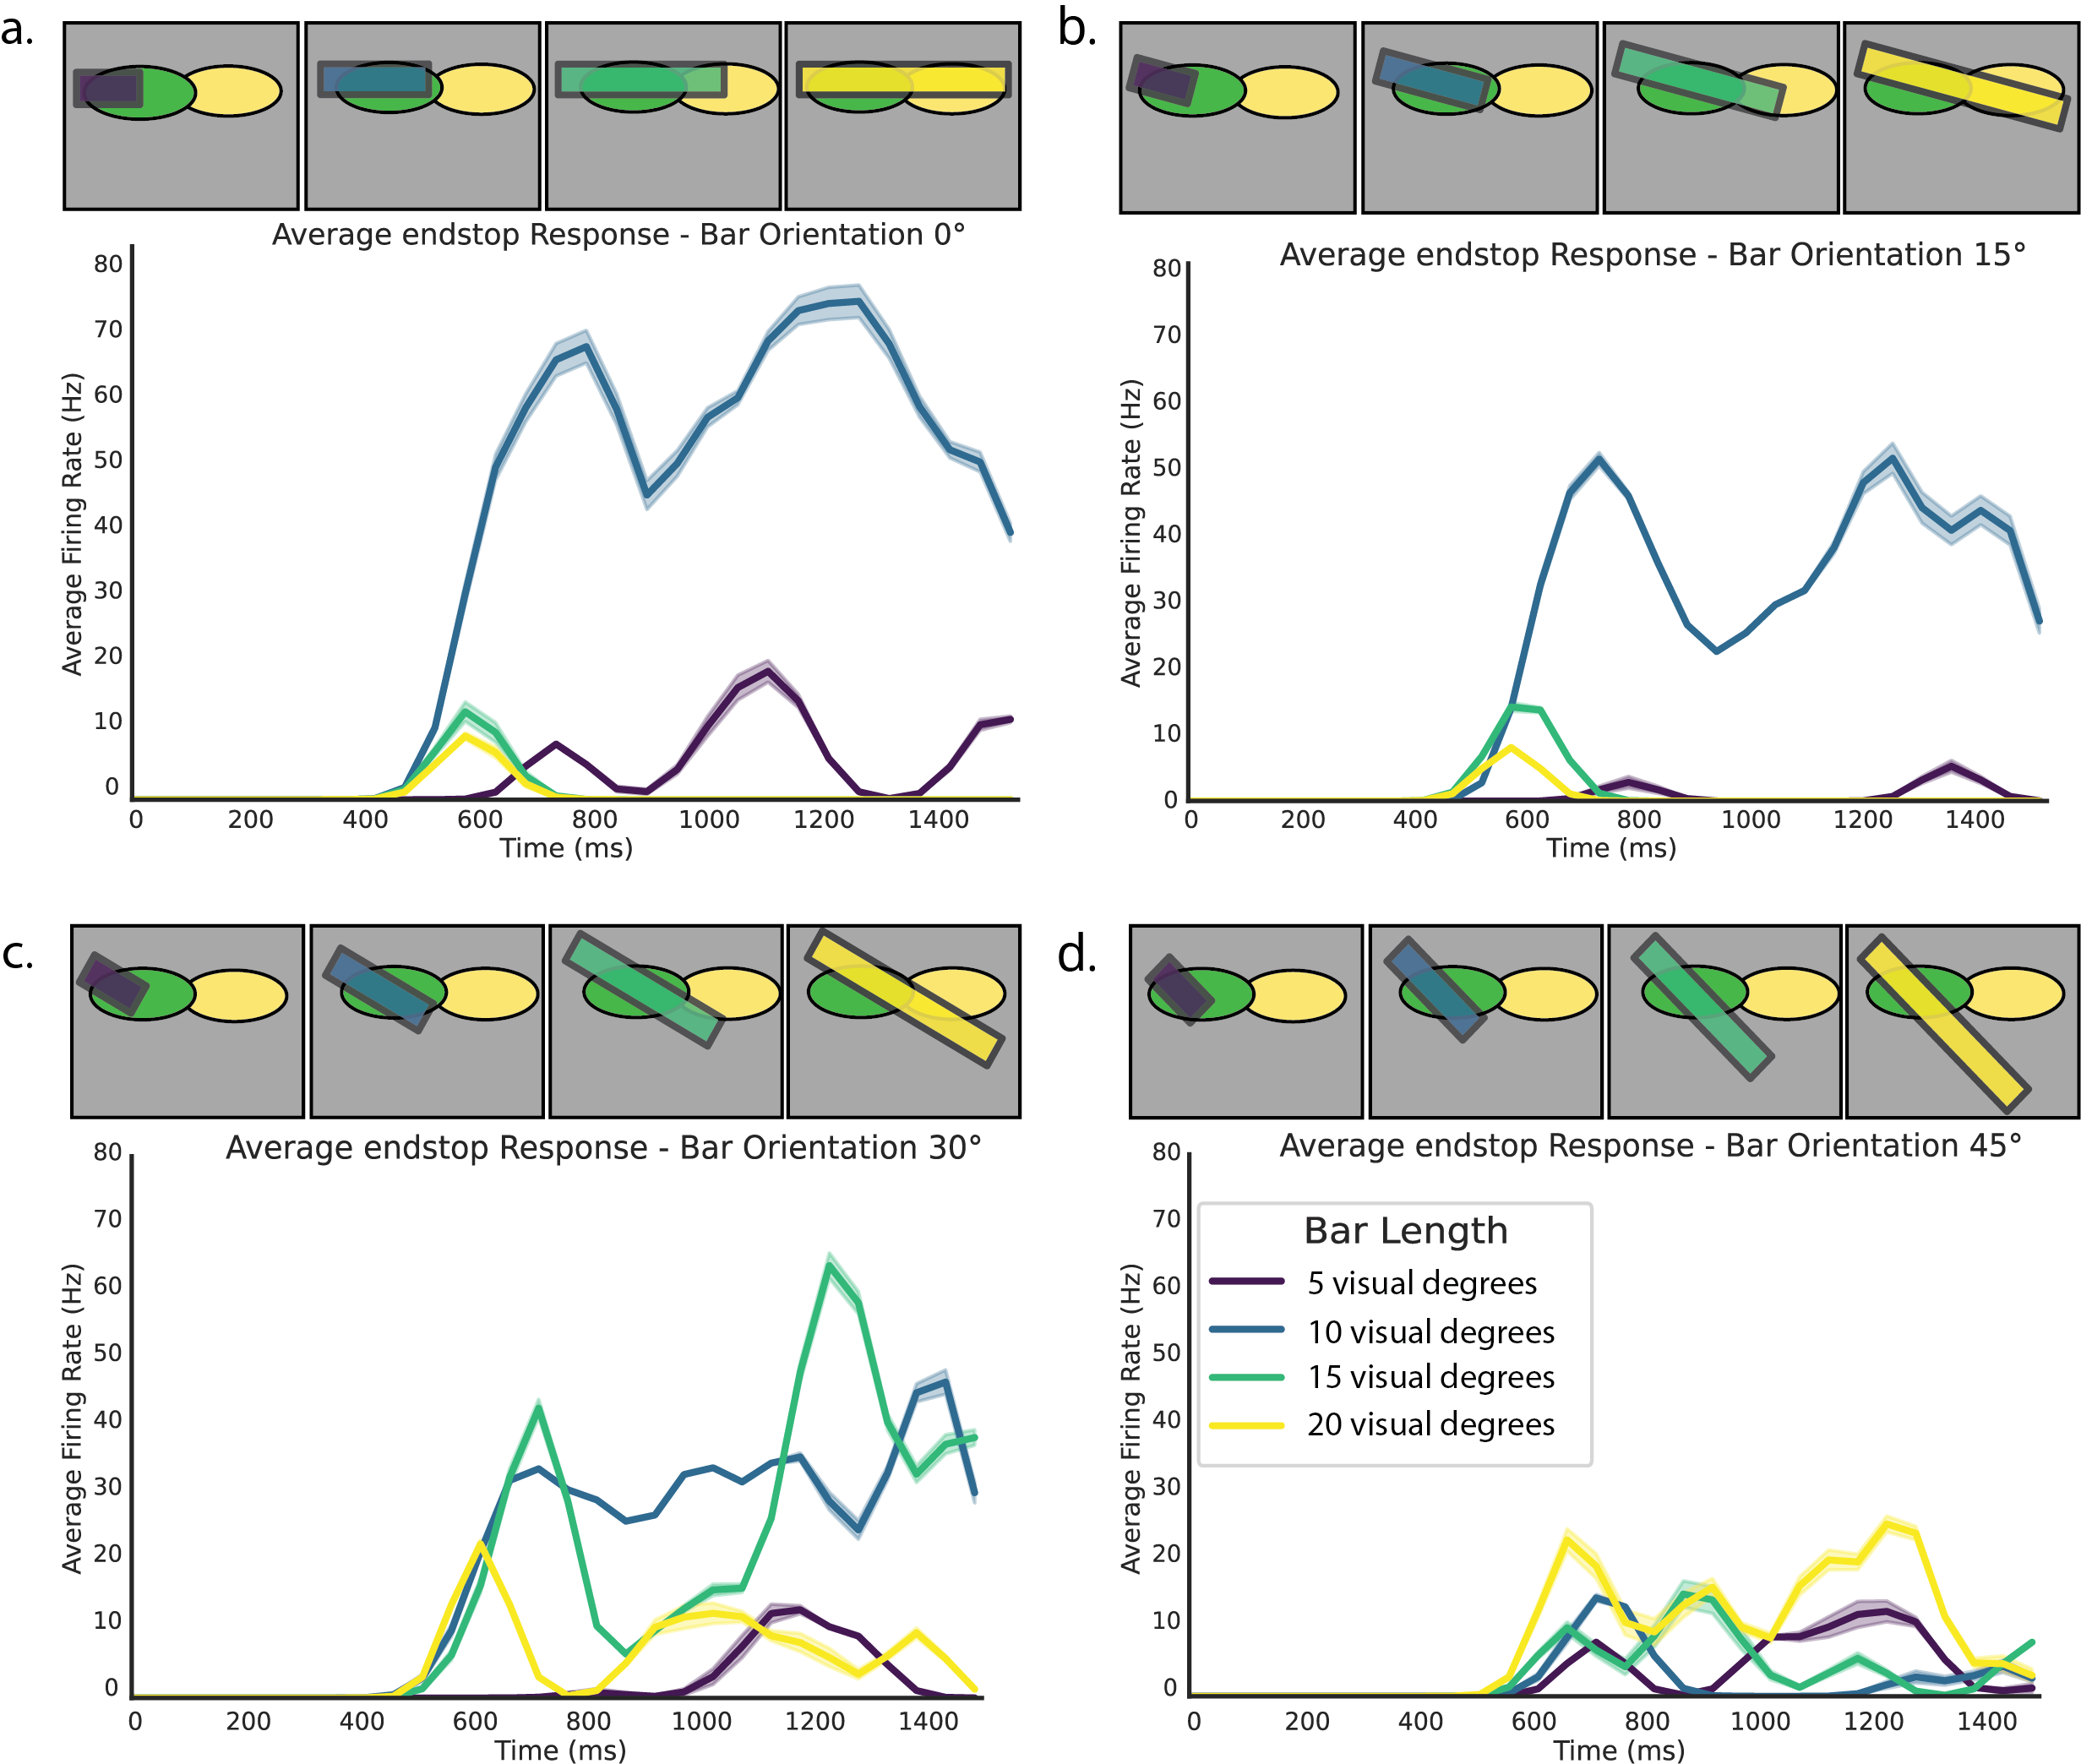
\includegraphics[width=1.0 \textwidth]{./adjusted_figures/LIF_endstopping_length_orientation.png}
    \caption{Neural responses of the endstopped complex cells to line segments with different lengths: 5, 10, 15, 20 visual degrees, and orientations 0°, 15°, 30°, 45°. a. The optimal endstopped response to a line with orientation 0°. A large difference in peak activity between length 10 and 20 visual degrees. The x-axis represents the simulation time, and the y-axis represents the firing rate of the complex cell in spikes per second (Hz). The cell types are colour coded according to stimulus length, and presented in the legend of panel d. b. The relative difference decreases when the line segment is rotated away from the preferred orientation. c. Endstopping decreases further and responses are more similar to complex cells. d. Endstopping is completely decreased as the line segment does not activate the end zone.}
    \label{fig:endstopping}
\end{figure}

To gain a better understanding of the neural dynamics within the circuit, we also stimulated the model with a continuously growing bar. This approach allows us to visualise subtle differences related to the length of the bar at the population's preferred orientation, as shown in \hyperref[fig:endstopping_length]{figure 10a}. This figure illustrates the elicited response of endstopped neurons to a bar that starts at the beginning of the receptive field and extends progressively into the endstopping inhibitory endzone. The line plot on the left shows the average firing rate in spikes per second (Hz) of the endstopped neurons as a function of bar length in visual degrees. The shaded area represents the variability around the mean firing rate. As depicted, the average firing rate increases steadily as the bar lengthens from 0 to approximately 15 visual degrees, peaking around 70 Hz. This peak indicates the optimal bar length that maximally activates the endstopped neurons within the receptive field. Beyond this length, the firing rate starts to decline, reflecting the inhibitory effect as the bar extends into the adjacent complex cell's receptive field. Importantly, \hyperref[fig:endstopping_length]{figure 10b} is a hypercomplex cell from cat V1 and the receptive fields of those cells are smaller and more responsive compared to mice. The length of the input bar can be seen on the x-axis. The figures on the right side of the figure provide a visual representation of the bar's interaction with the receptive fields at different stages of its growth. The top inset shows the bar initially positioned within the receptive field of the endstopped neuron, eliciting a strong response. The middle inset illustrates the bar extending into the inhibitory zone, where the inhibitory feedback begins to reduce the firing rate. Finally, the bottom inset depicts the bar fully extending into the adjacent complex cell's receptive field, resulting in a significant reduction in the firing rate due to maximal inhibition. This figure effectively captures the dynamic response of endstopped neurons to varying bar lengths, highlighting the intricate balance between excitation and inhibition within the microcircuit. It reinforces the notion that recurrent inhibition plays a crucial role in modulating the activity of endstopped neurons, particularly in response to stimuli that extend beyond their classical receptive fields.

  \begin{figure}[H]
    \centering
    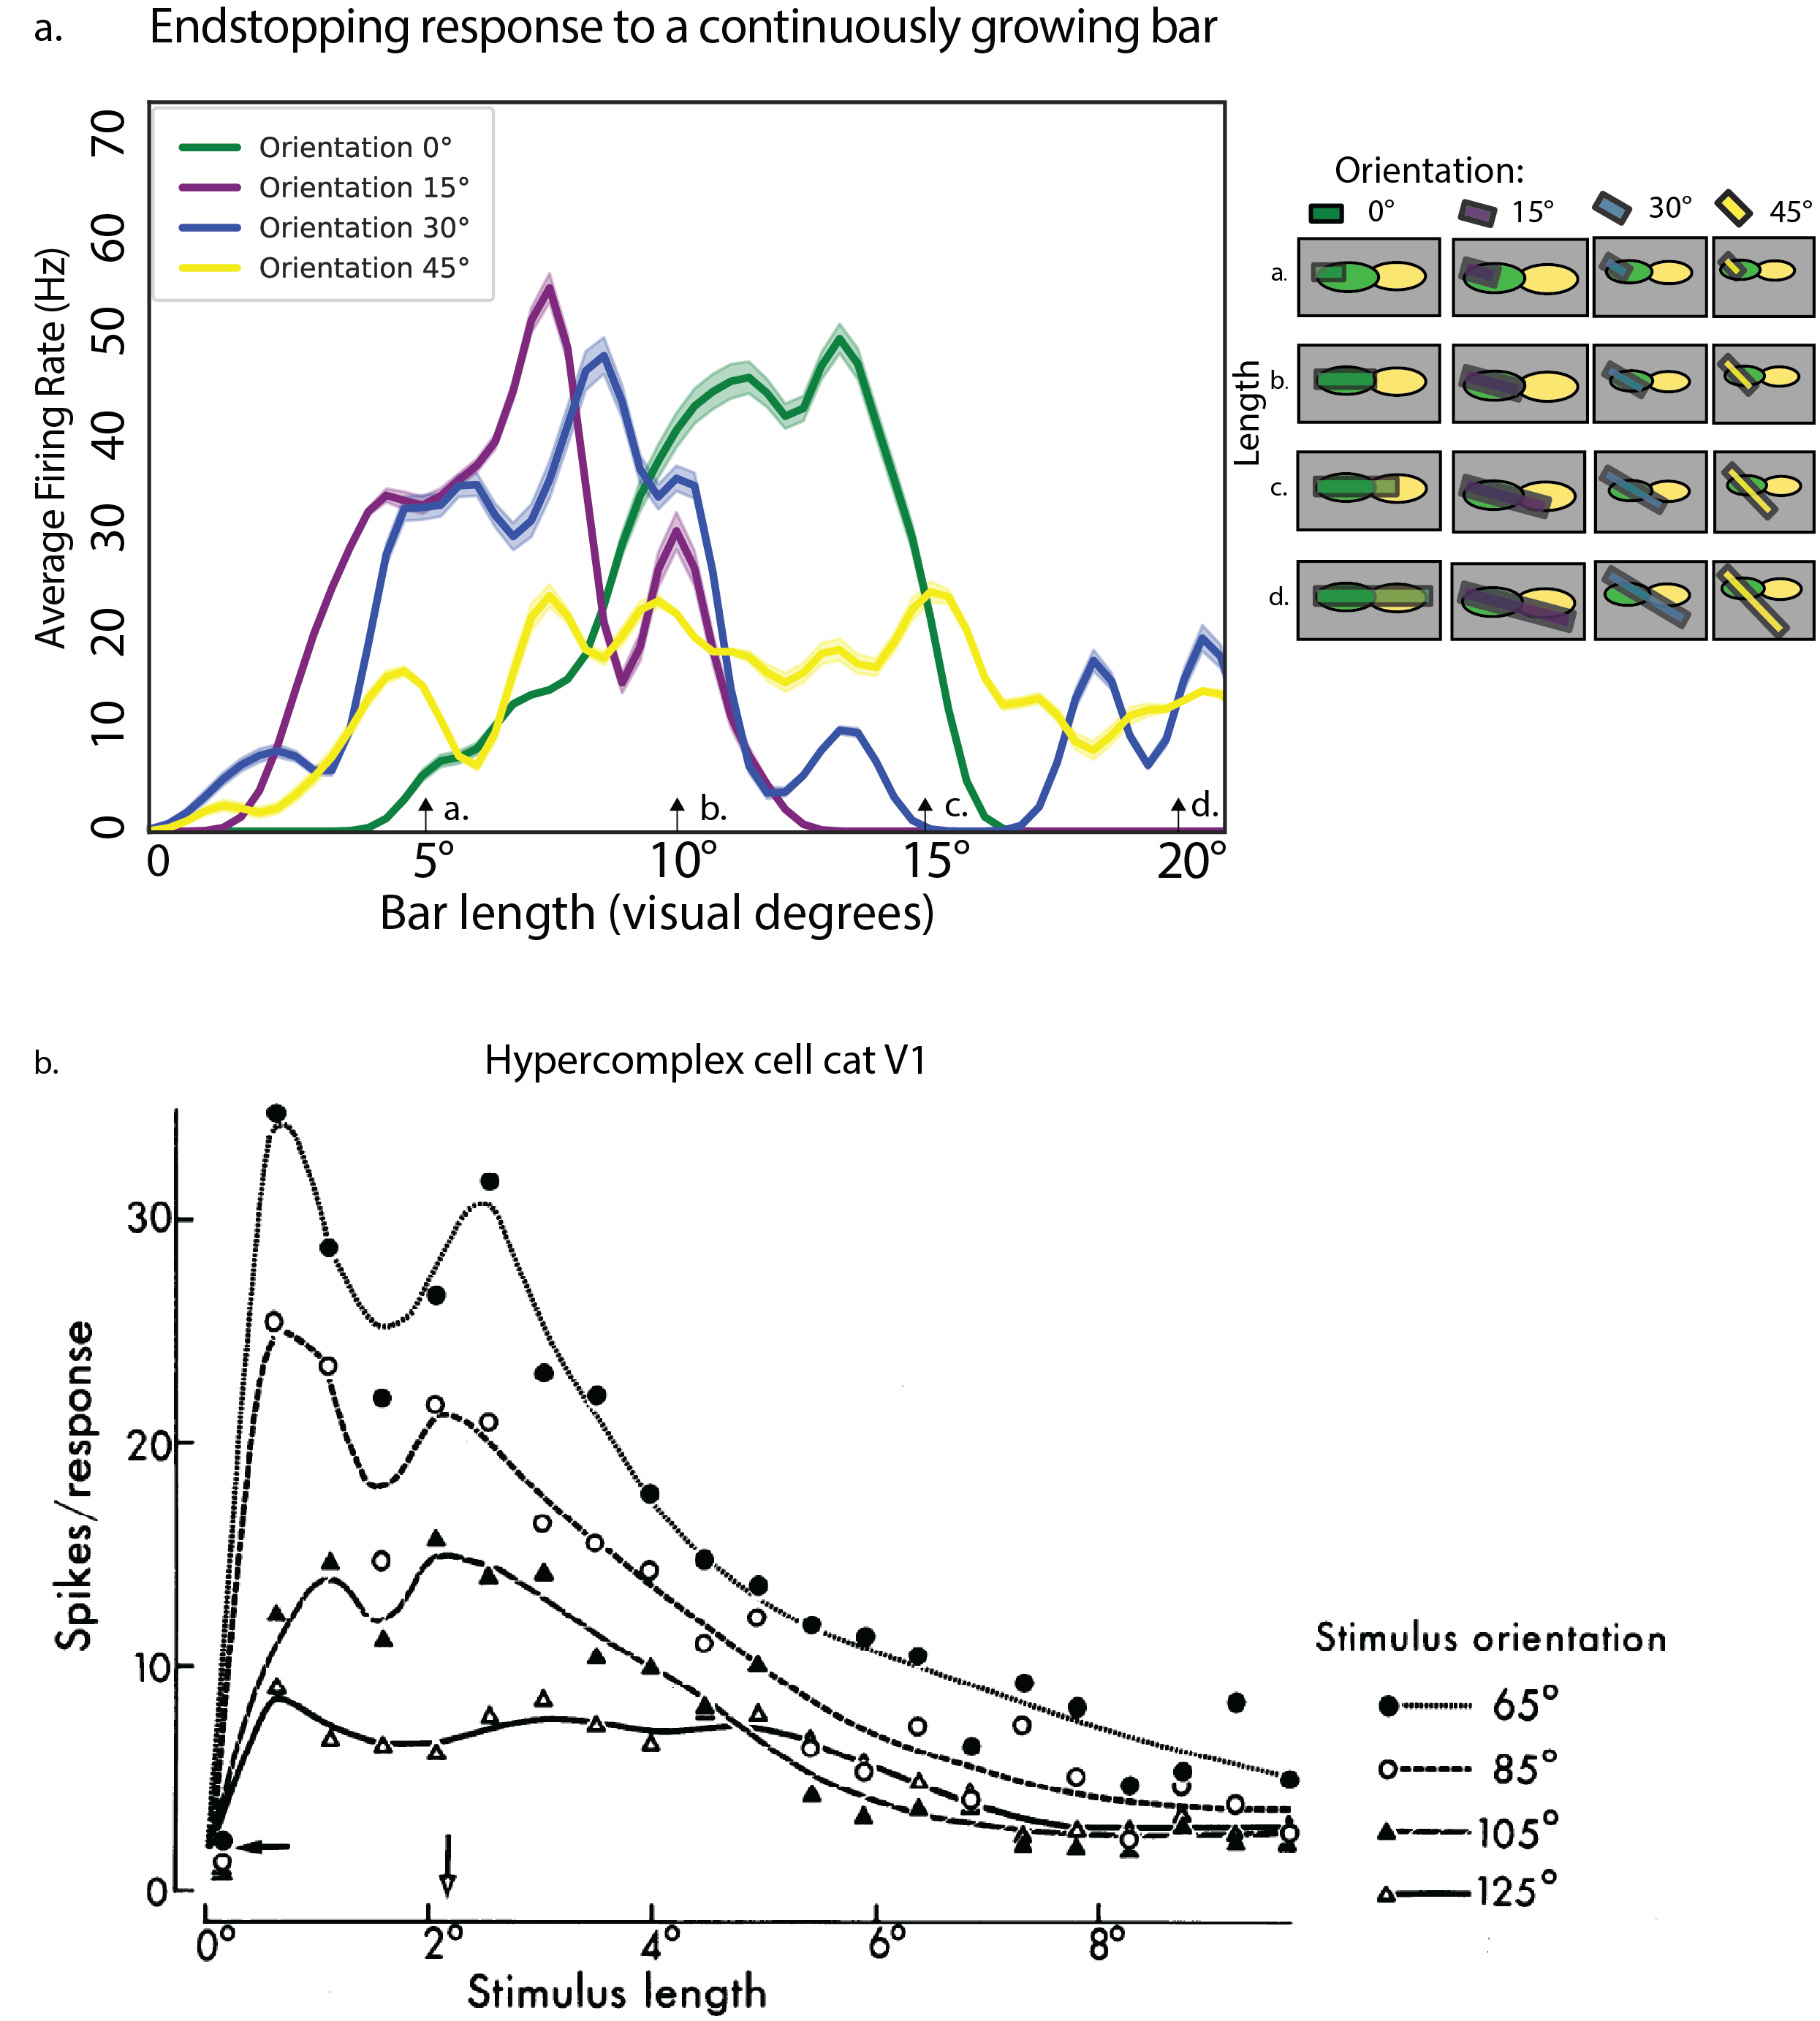
\includegraphics[width=1.0 \textwidth]{adjusted_figures/endstop_line_length_physiology.png}
    \caption{a. The responses of an endstopping population stimulated with a continuously growing bar. The population has a preferred orientation of 0°. The response to the 0° line segment shows that the firing rate slowly ramps up to a maximum of 50 Hz, to the line being around 12 visual degrees, after which firing rate is quickly decreased for longer inputs. b. The endstopped response of a physical hypercomplex or endstopped cell in cat V1. The receptive field sizes of cat V1 hypercomplex are smaller than that found in the mouse. Panel b. was taken from \textcite{orbanDimensionsPropertiesEndzone1979}.}
    \label{fig:endstopping_length}
  \end{figure}

  % To further quantify the endstopping mechanism as influenced by different cell types, we analysed the average endstopping responses of networks with varying compositions of endstopped cells. Specifically, we investigated networks with 1, 5, 10, 20, and 40 endstopped cells while adjusting the ratios of other cell types to observe the resulting endstopping responses \hyperref[fig:endstop_network]{figure 11}. Network 1, with a minimal configuration, included 1 endstopped cell, 1 complex cell, 20 simple cells, and 5 PV interneurons. In Network 5, the composition was adjusted to 5 endstopped cells, 5 complex cells, 50 simple cells, and 10 PV interneurons. Network 10 featured a balanced mix of 10 endstopped cells, 10 complex cells, 100 simple cells, and 20 PV interneurons. Network 20, which demonstrated the highest endstopping accuracy, consisted of 20 endstopped cells, 20 complex cells, 500 simple cells, and 50 PV interneurons. Finally, Network 40, the largest configuration, was composed of 40 endstopped cells, 40 complex cells, 1000 simple cells, and 200 PV interneurons. Among these configurations, Network 20 achieved the highest endstopping accuracy, with an \( r^2 \) value of 0.65. Notably, this network maintained a PV to simple cell ratio of 1:10, suggesting the optimal balance between PV and simple cells for endstopping accuracy in our LIF model.
To further quantify the endstopping mechanism influenced by different cell types, we analysed the average endstopping responses of networks with varying compositions of endstopped cells. We investigated networks with 1, 5, 10, 20, and 40 endstopped cells while adjusting the ratios of simple cells to PV cells to observe the resulting endstopping responses. Specifically, Network 1 included 1 endstopped cell, 1 complex cell, 20 simple cells, and 10 PV interneurons (1:2). In Network 5, the composition was adjusted to 5 endstopped cells, 5 complex cells, 50 simple cells, and 10 PV interneurons (1:5). Network 10 featured a balanced mix of 10 endstopped cells, 10 complex cells, 100 simple cells, and 20 PV interneurons (1:5). Network 20, which demonstrated the highest endstopping accuracy, consisted of 20 endstopped cells, 20 complex cells, 500 simple cells, and 50 PV interneurons (1:10). Finally, Network 40 was composed of 40 endstopped cells, 40 complex cells, 1000 simple cells, and 50 PV interneurons (1:20).

The Mann-Whitney U test results revealed significant differences in SNR values between several network configurations, with Network 20 showing particularly notable differences. Specifically, comparisons between Network 20 and other networks indicated significant differences: Network 1 vs. Network 20 ($U = 0.0$, $p = .026$), Network 5 vs. Network 20 ($U = 0.0$, $p < .001$), Network 10 vs. Network 20 ($U = 0.0$, $p < .001$), and Network 20 vs. Network 40 ($U = 800.0$, $p < .001$). These results suggest that the SNR values in Network 20 are distinctly different from those in Networks 1, 5, 10, and 40. Among these configurations, Network 20 achieved the highest endstopping accuracy, with an $r^2$ value of 0.67, maintaining a PV to simple cell ratio of 1:10, indicating the optimal balance between PV and simple cells for endstopping accuracy in our LIF model.

\begin{figure}[H]
  \centering
  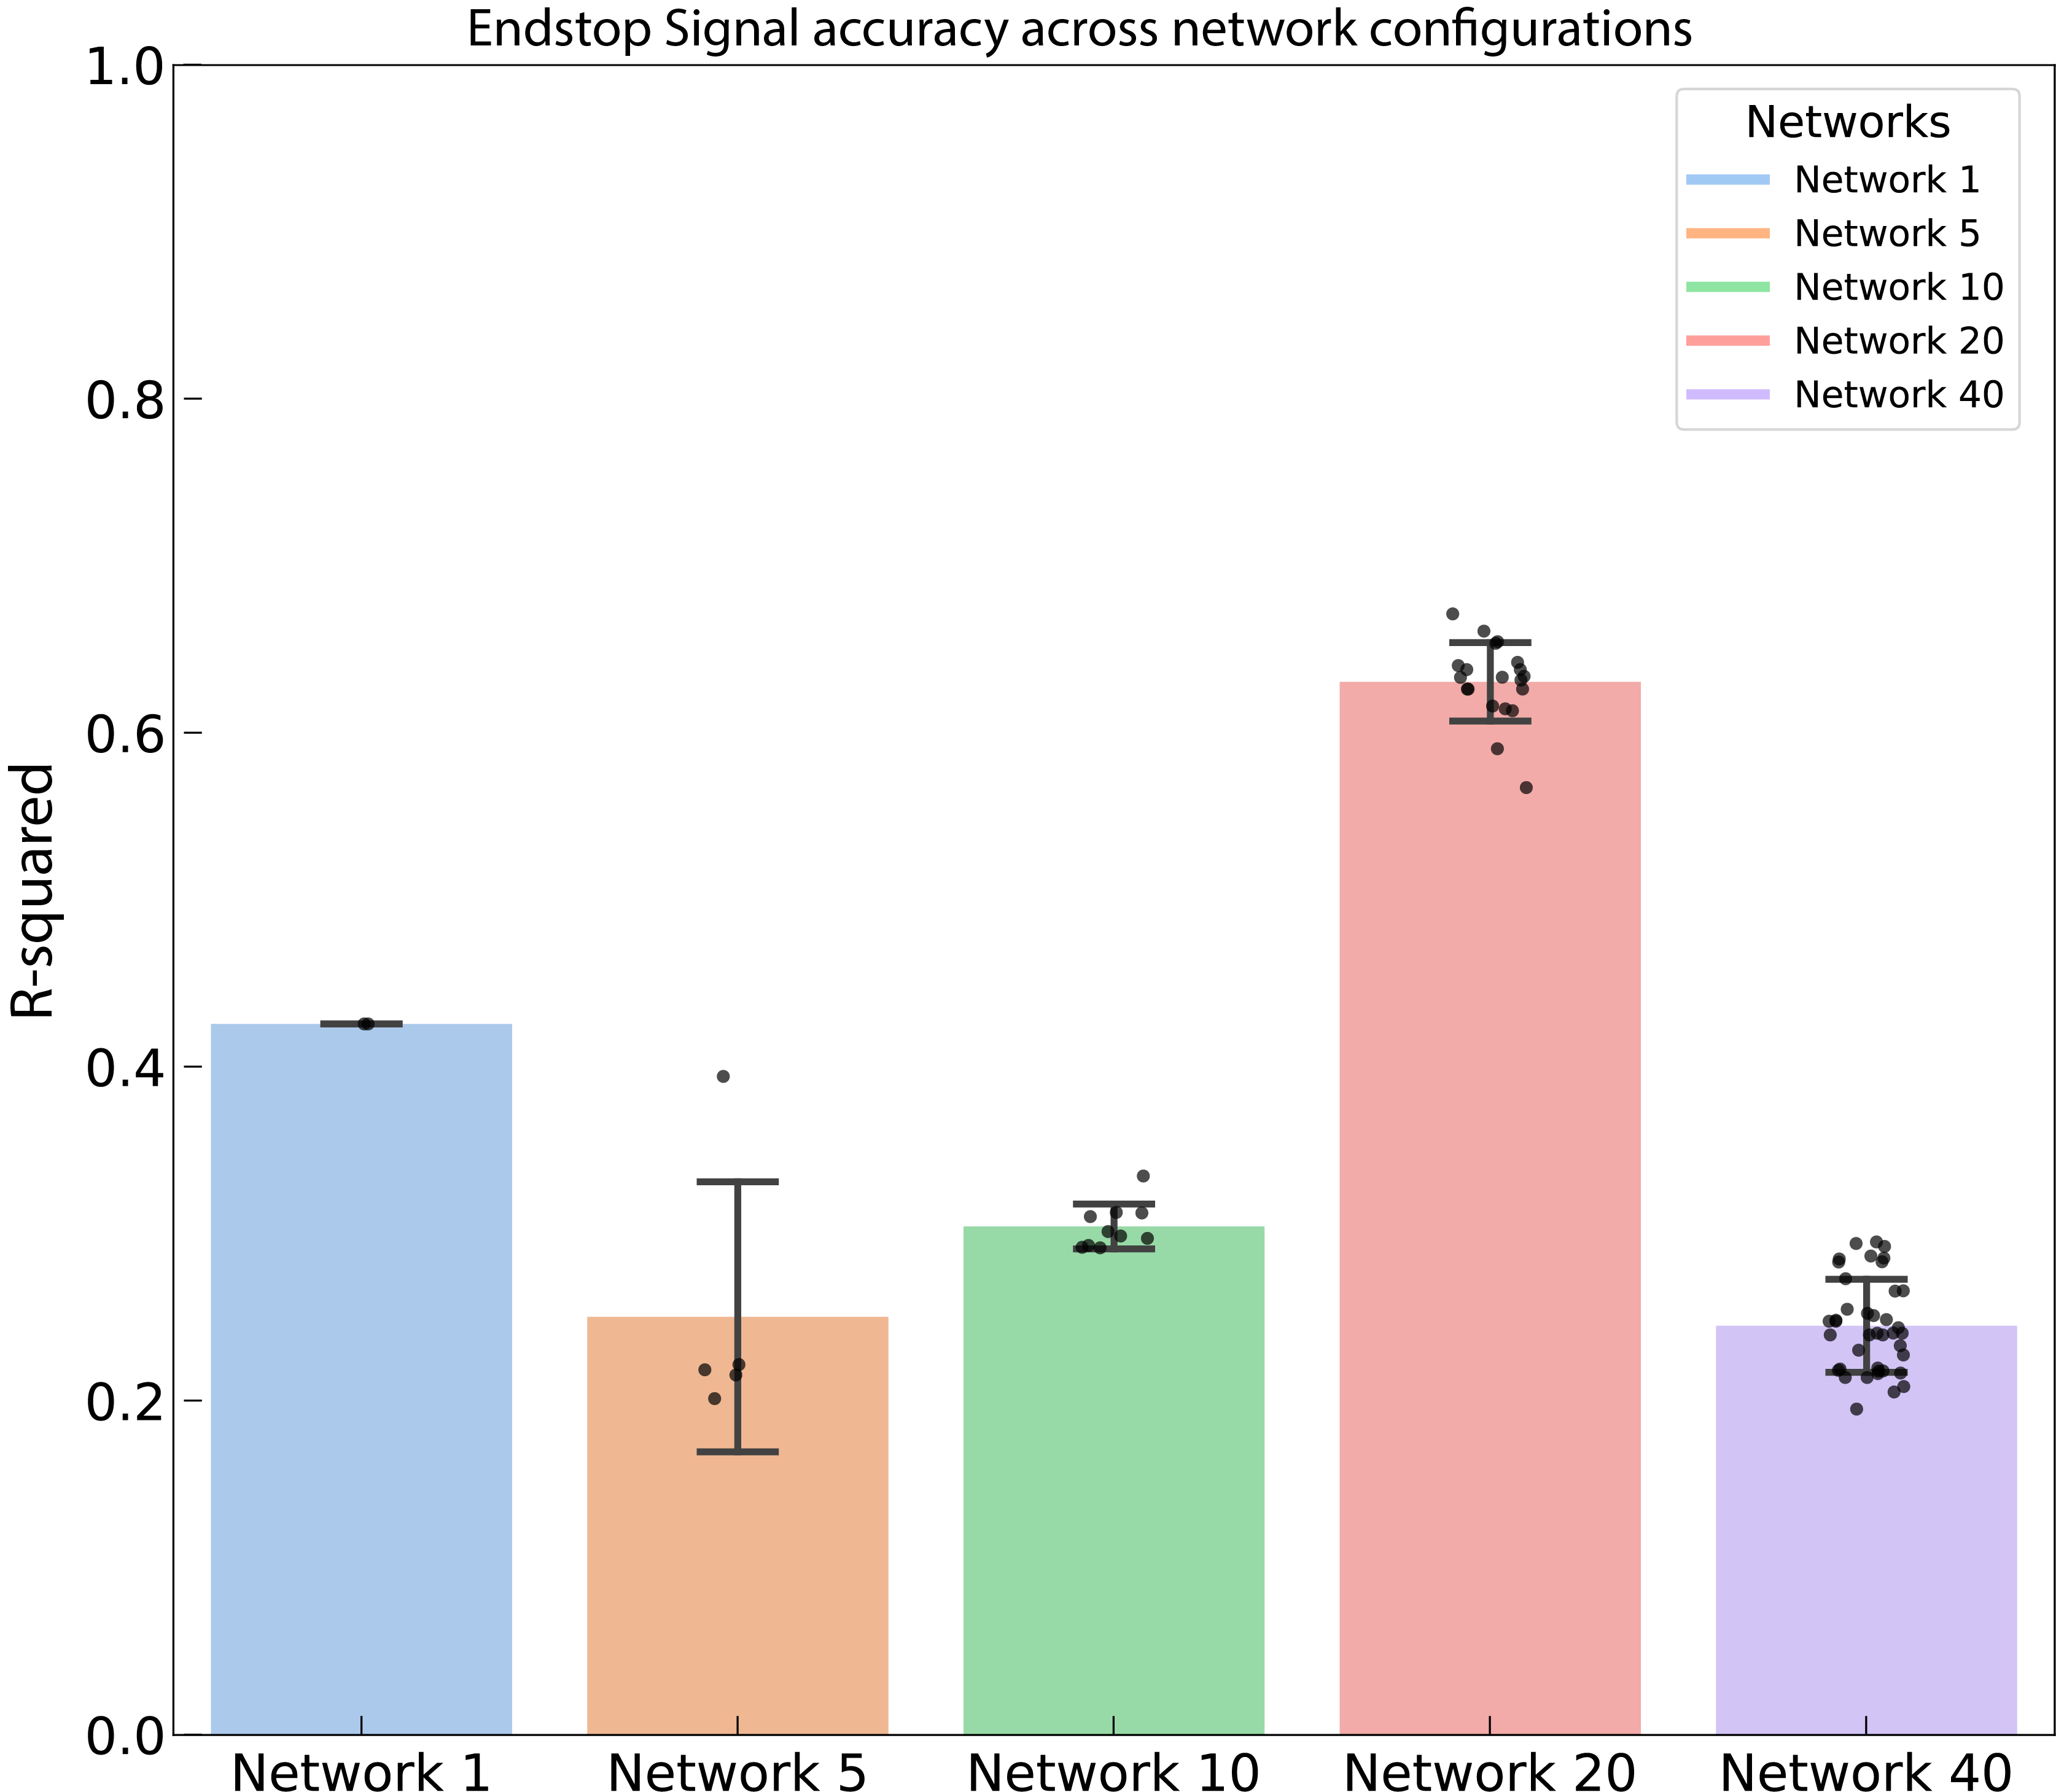
\includegraphics[width=1.0 \textwidth]{adjusted_figures/figure_networks_bar.png}
  \caption{The average endstopping responses of networks with 1, 5, 10, 20, and 40 endstopped cells were analysed. Endstopping accuracy was quantified by fitting a quadratic polynomial to the smoothed PSTH response to a bar continuously increasing in length along the cell's preferred orientation. The network with 20 endstopped cells exhibited the highest endstopping accuracy, with a PV to simple cell ratio of 1:10.}
  \label{fig:endstop_network}
\end{figure}
  %ToDo rewrite population model description
%\subsection{Population activity illusory contours}
Next, we examined whether our population model reflected results found during physiological experiments done with the abutting grating illusion \autocite{vonderheydtMechanismsContourPerception1989}. They showed that the illusory contour breaks down when a gap is introduced misaligning the horizontal inducers. Additionally, they demonstrated that when a bar crosses the illusory line illusory responses decreased as well. Figure \ref{fig:population_contours} showcases the responses of different cell types to visual stimuli designed to induce the perception of illusory contours. The left panels of each sub-figure (a, b, and c) display the mean firing rates of various cell populations, including complex cells tuned to 90 degrees for the illusory response, complex cells tuned to 0 degrees that are tuned for the inducers and to create endstopped cells, and pattern cells used to integrate signals from the endstopped cells. The right panels depict the spatial arrangement and the type of stimulus presented, which varies across the sub-figures.
\bigbreak
% In subfigure (a), the stimulus arrangement created a strong illusion of contours aligned with the orientation preference of the complex 90 cells. This is evidenced by the robust mean firing rate of the complex cells tuned to 90 degree orientations peaking at around 30 Hz, indicating a high level of activity in response to the perceived illusory contours. The elevated firing rates suggest that these cells are effectively encoding the illusion, signaling the presence of a boundary where none exists in the physical stimulus. When the stimulus is altered to disrupt the illusion, as seen in subfigures (b) and (c), the activity of the complex 90 cells changes significantly. In subfigure (b), the stimulus modification appears to partially disrupt the illusory contour. This is reflected in the reduced firing rate of the complex cells tuned to 0 degree input compared to subfigure (a), though the response remains notable. This partial disruption suggests that the illusory contour is weakened but not entirely broken, resulting in a moderate decrease in the encoding efficiency of these cells.

In subfigure (a), the stimulus created a strong illusion because inducers were horizontally matching the orientation preference of complex 0° endstopped cells and were vertically aligned, so the pattern cell was maximally stimulated. The robust mean firing rate of the complex 90° cells, peaking around 40 Hz, suggested effective encoding of the perceived illusory contours. When the stimulus is modified in sub-figures (b) and (c) to disrupt the illusion, the complex 90° cells' activity changes significantly. Sub-figure (b) shows a partial disruption of the illusion, reflected in a reduced firing rate of the complex cells, though the response remained around baseline, indicating a potential for illusory contour but not enough to effectively activate the pattern cell population.
\bigbreak
In sub-figure (c), the stimulus is further modified, to completely break the illusion. The firing rate of the complex 90° cells drops significantly compared to sub-figures (a) and (b). This substantial reduction in activity indicates that the complex 90 cells are no longer effectively encoding the illusory contour, as the stimulus no longer supports the perception of such a contour. The response of these cells now aligns more closely with their response to an actual absence of contours, highlighting their role in specifically detecting and encoding illusory boundaries. The right panels of each sub-figure visually illustrated the stimulus configurations, showing how the spatial arrangement of elements impacts the perception of illusory contours. The colour coding indicates the average firing rates, with warmer colours representing higher activity levels. The complex cells (dotted outlines) and end-stop cells (solid outlines) are shown in their spatial positions, providing a visual representation between cell type, location, and stimulus-induced activity.
\bigbreak
In summary, the complex 90 cells are crucial for encoding illusory contours, as evidenced by their high firing rates in response to stimuli that induce such perceptions. When the stimulus is altered to disrupt the illusion, the activity of these cells decreases accordingly. This suggests that the complex 90 cells are finely tuned to detect and encode the presence of contours, whether real or illusory, and their activity is a direct reflection of the strength of the perceived illusion. These findings underscore the importance of specific neural populations in the higher-order processing of visual information, particularly in the context of perceptual phenomena like illusory contours.

\begin{figure}[H]
  \centering
  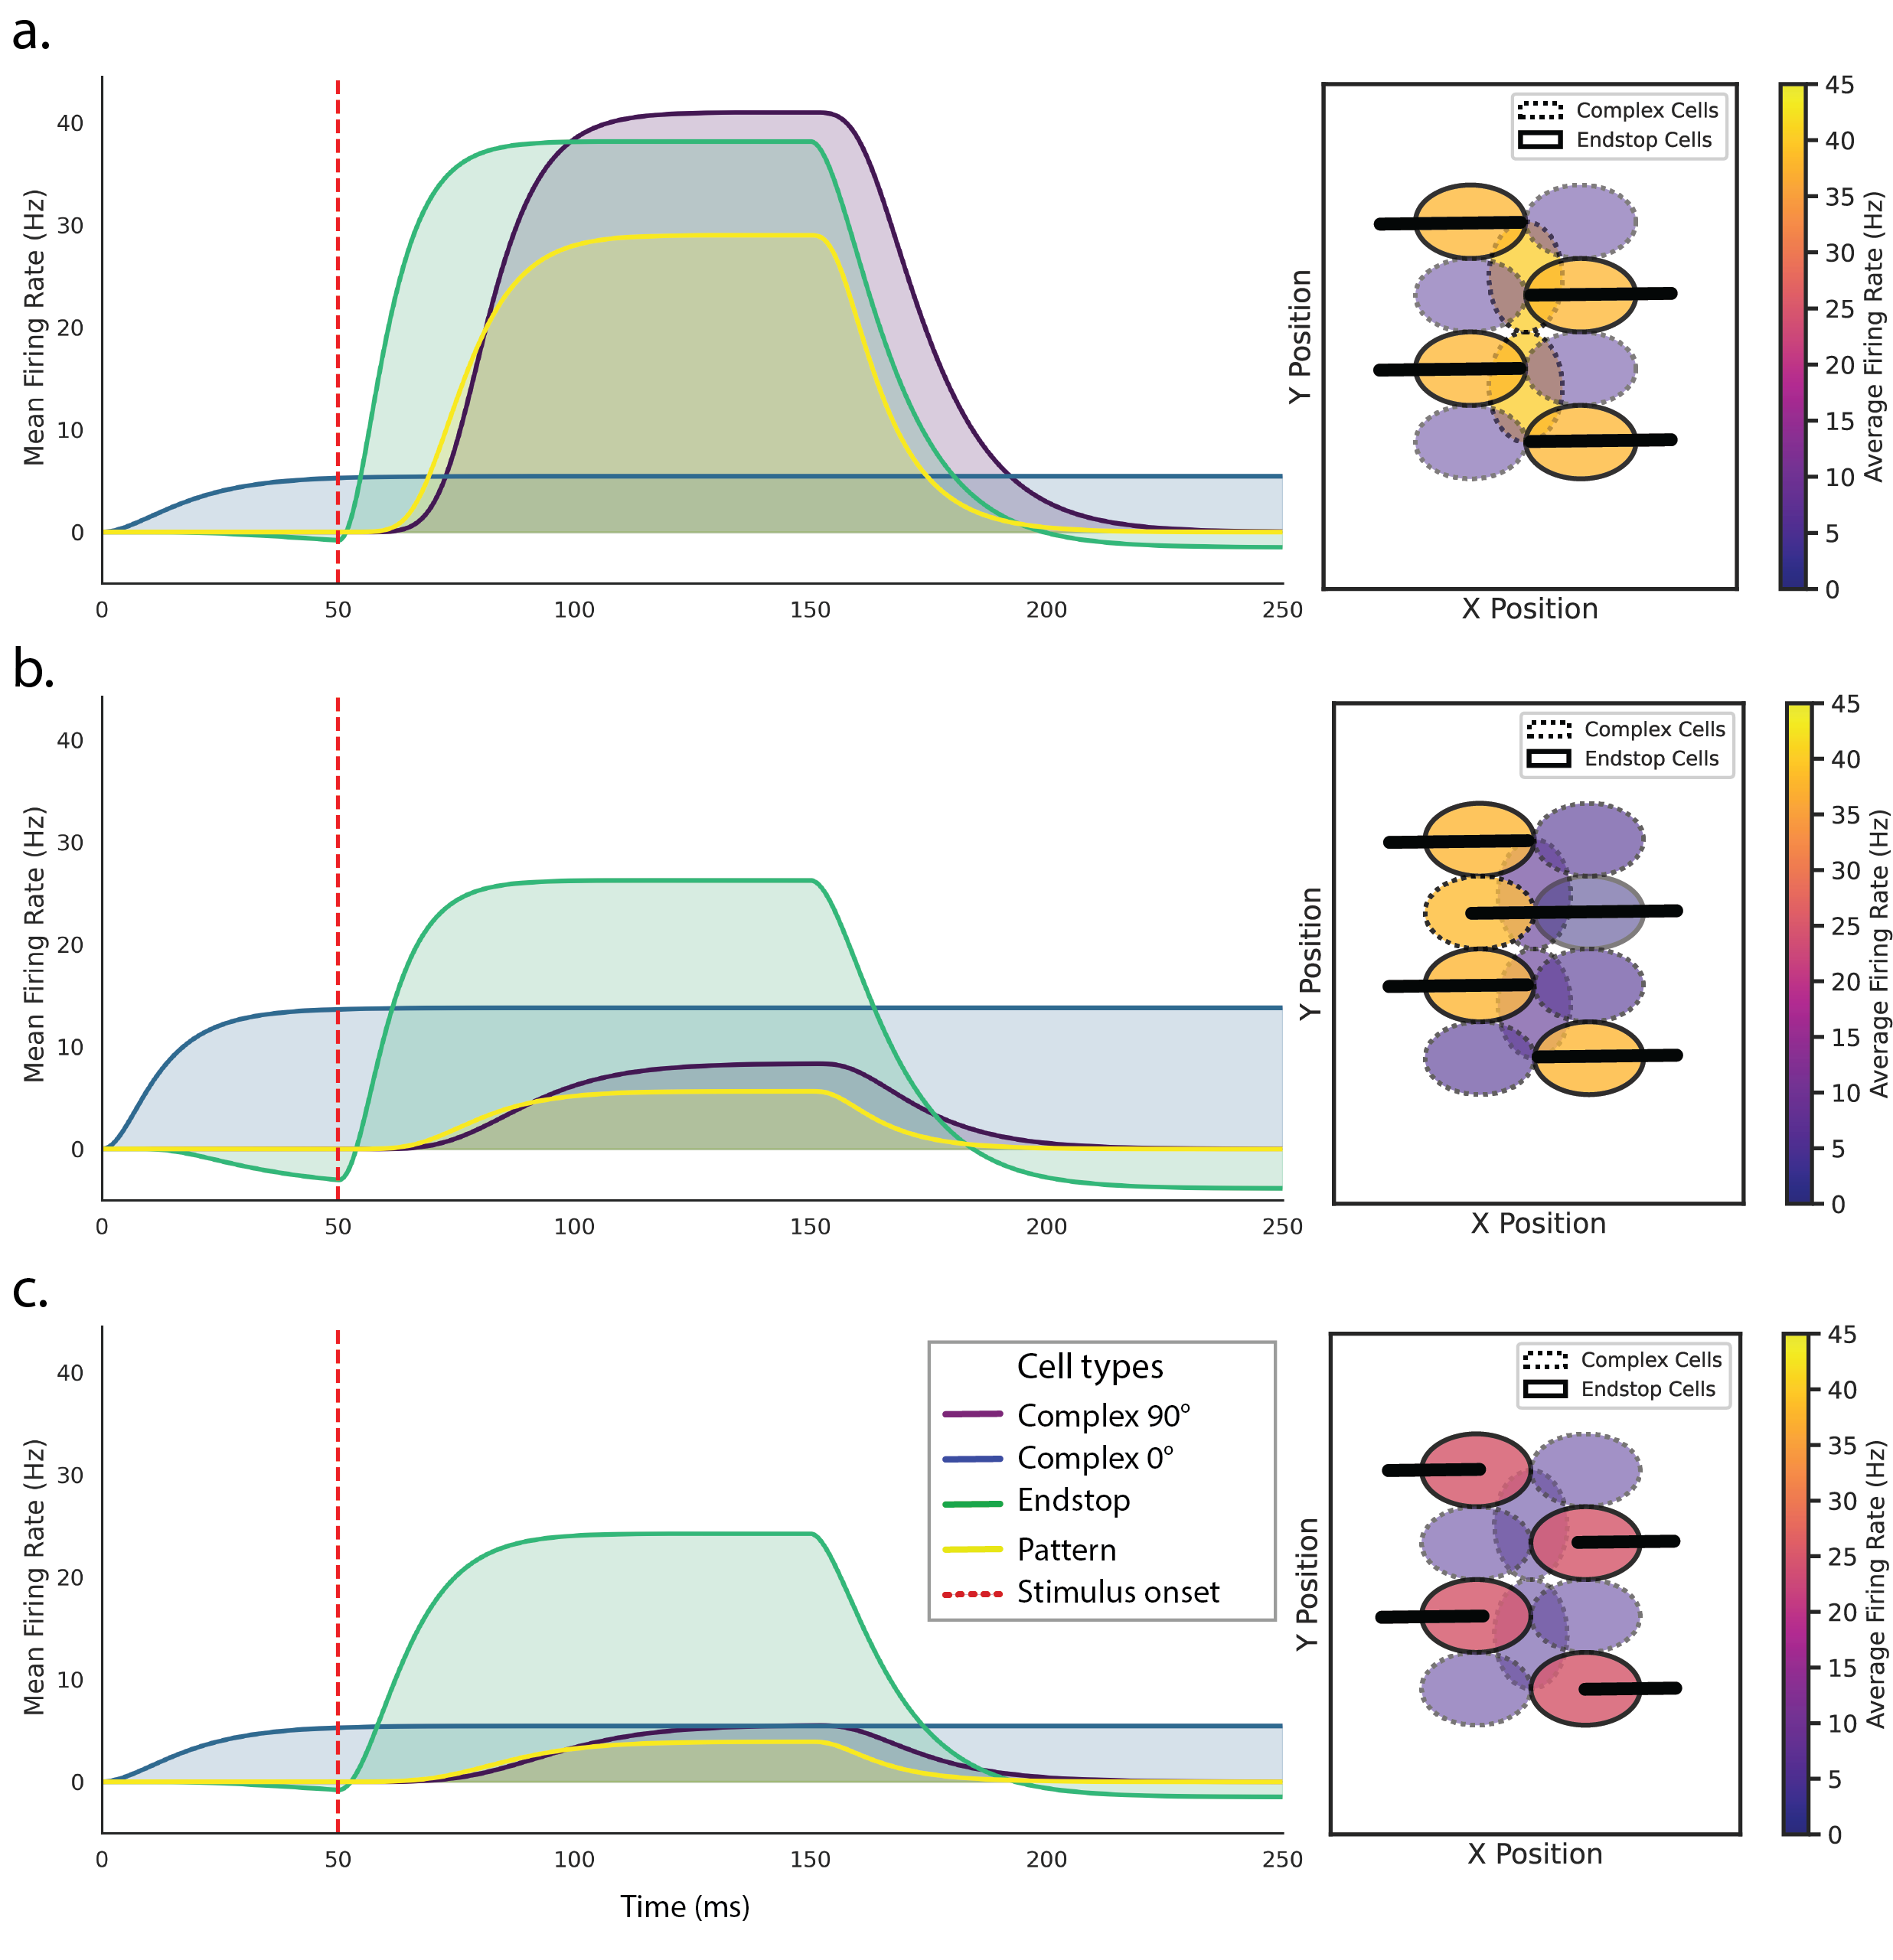
\includegraphics[width=1.0 \textwidth]{adjusted_figures/Figure_Population.png}
  \caption{Population responses to the abutting grating illusion. a. The optimal input is given to the model, all inducers are the preferred orientation and are spatially aligned. All endstopped populations are very active, and the complex end zones are not active, thus resulting in maximum representation of the illusory contour. b. In this example one of the inducers crosses the illusory contour, resulting in the abolishment of the illusion. The complex end zones increase in activity and thus the activity of the endstopped cell also decreased, and no illusory contour is formed. c. Similarly, in this figure the inducer lines are not aligned enough the form a strong illusory contour. The complex end zones are not activated, but also the endstopped cells are not maximally stimulated. Therefore, the pattern cell is not stimulated and no illusory contour is formed.}
  \label{fig:population_contours}
\end{figure}

\newpage
\section*{Discussion}
\setlength{\parindent}{12pt}  
The current models demonstrated that endstopping can be generated through recurrent inhibitory connectivity and can be effectively integrated by higher visual areas to drive recurrent contour completion. We modelled endstopped cells by creating a LIF-microcircuit of two adjacent populations of complex cells connected through inhibitory feedback on the simple cell level. The inhibitory feedback resulting in a decrease in firing whenever a stimulus edge is extended beyond the excitatory endstop receptive field into the inhibitory end zone. This LIF-model demonstrated that the endstopped cells are a critical first step for the detections of illusionary inducing local features. To examine how the global representation of the abutting grating illusion is formed we used a second model that implemented population firing rate model equations. This population model had a similar architecture as that was used in the LIF-model, but with the extension to a higher visual area LM. The abstraction from point neurons to neural populations ensured a stable firing rate without the need for extensive weight tuning between individual cells. Still, the population model had a similar architecture as compared to the LIF-model; in which endstopping microcircuits were made from combined simple, complex, and inhibitory cells. Results from the population model demonstrated that endstopped signals can be used to group retinotopically aligned inducers into a global illusory representation by recurrently amplifying feedback signals originating from LM. 
\setlength{\parindent}{0pt}
\bigbreak

% Inhibition plays a vital role in both the LIF and population models, where PV interneurons play a major role in visual processing, shaping how sensory information is processed. In the context of the LIF model, endstopped cells are influenced by direct excitation from feedforward inputs and indirect inhibition through recurrent feedback connections. These inputs form distinct receptive fields, a feedforward classical receptive field and a retinotopically offset receptive field that functions as an inhibitory endzone. In alignment with observations from \textcite{sillitoContributionExcitatoryInhibitory1977}, inhibitory influences are not exerted directly at the level of the endstopped cells. We propose that the segregation of inhibition serves a functional purpose to generate stable endstopping. Current results showed by varying the stimulus length and orientation that endstopping is gradually reduced when stimuli diverged from its optimal configuration, and we propose that PV interneurons play a pivotal role in modulating excitatory and inhibitory interactions. The indirect inhibitory feedback, facilitated by PV interneurons, allows for a more adaptable and nuanced modulation of the excitatory signals depending on the visual context. This adaptive modulation is crucial, especially when the visual stimuli vary in length and orientation, leading to changes in the perceived endstopping effect. The dynamic regulation by PV interneurons helps maintain a balance that can prevent excessive excitatory activity that might otherwise lead to neural saturation or noise dominance in the signal processing.

% Moreover, the organisation of synaptic weights in PV interneurons, as described by \textcite{znamenskiyFunctionalSpecificityRecurrent2024}, highlights the functional benefits of indirect inhibition used in the current model. By preferentially inhibiting those pyramidal neurons that share similar visual selectivities and provide strong excitatory feedback, PV interneurons not only suppress potential excitatory overshoots but also enhance the overall selectivity and sharpness of neural responses. This targeted inhibition is essential for refining the output of neural assemblies, ensuring that the response patterns are both specific and contextually appropriate. Furthermore, the ability of endstopped cells to adjust their firing patterns based on contrast variations could offer insights into the mechanisms underpinning contrast sensitivity in their second order spiking features, suggesting a complex interplay between inhibition and sensory perception.

Inhibition plays a vital role in both the LIF and population models, with PV interneurons being crucial in visual processing by shaping how sensory information is managed. In the context of the LIF model, endstopped cells are influenced by direct excitation from feedforward inputs and indirect inhibition through recurrent feedback connections. These inputs form distinct receptive fields: a feedforward classical receptive field and a retinotopically offset receptive field functioning as an inhibitory endzone. As observed by \textcite{sillitoContributionExcitatoryInhibitory1977}, inhibitory influences are not exerted directly at the level of the endstopped cells. The segregation of inhibition serves a functional purpose in generating stable endstopping. Current results showed that varying the stimulus length and orientation gradually reduces endstopping when stimuli diverge from its optimal configuration \hyperref[fig:endstopping_length]{figure 10 a}, highlighting the role of PV interneurons in modulating excitatory and inhibitory interactions.

The indirect inhibitory feedback facilitated by PV interneurons allows for adaptable and nuanced modulation of excitatory signals depending on the visual context. This adaptive modulation is crucial when visual stimuli vary in length and orientation, leading to changes in the perceived endstopping effect. The dynamic regulation by PV interneurons helps maintain a balance, preventing excessive excitatory activity that might otherwise lead to neural saturation or noise dominance in signal processing. Furthermore, the organisation of synaptic weights in PV interneurons, as described by \textcite{znamenskiyFunctionalSpecificityRecurrent2024}, underscores the functional benefits of indirect inhibition used in the current model. By preferentially inhibiting pyramidal neurons that share similar visual selectivities and provide strong excitatory feedback, PV interneurons suppress potential excitatory overshoots and enhance the overall selectivity and sharpness of neural responses.

This targeted inhibition is essential for refining the output of neural assemblies, ensuring that response patterns are specific and contextually appropriate. Additionally, the ability of endstopped cells to adjust their firing patterns based on contrast variations offers insights into the mechanisms underpinning contrast sensitivity in their second-order spiking features, suggesting a complex interplay between inhibition and sensory perception. Overall, PV interneurons provide stability to network dynamics by maintaining a balanced excitatory-inhibitory interaction, essential for precise and reliable sensory processing.

The ratio of 1:10 PV interneurons to simple cells roughly fits the observation of 10\% to 15\% of the primary visual cortex in the mouse \autocite{meyerInhibitoryInterneuronsCortical2011}. In the mouse primary visual cortex, this ratio is critical for maintaining the delicate balance between excitation and inhibition that is necessary for stable and accurate sensory processing. The relatively sparse population of PV interneurons compared to the more numerous simple cells allows for targeted and efficient inhibitory control. This configuration ensures that PV interneurons can effectively regulate the excitatory activity of a larger population of simple cells, thereby preventing runaway excitation and maintaining the stability of network dynamics.

Moreover, this specific ratio allows for precise temporal and spatial control over excitatory inputs, facilitating the sharp tuning of visual responses. By inhibiting specific pyramidal neurons and modulating their activity based on the visual context, PV interneurons contribute to the overall selectivity and responsiveness of the visual cortex. This selective inhibition is essential for processing complex visual stimuli and for the formation of accurate and contextually appropriate visual perceptions. The 1:10 ratio thus reflects an optimised balance that supports the functional architecture of the primary visual cortex, enabling mice to efficiently process and respond to their visual environment.


%Talking about the comparison to physiology endstopped cells of the cat


%\subsection{Recurrent inhibition can provide endstopped cells with information about sign of contrast.} % simple cell \autocite{yazdanbakhshEndStoppingV12006}
\textbf{ Endstopping is observed in both simple and complex cells within the visual cortex, presenting a paradox within complex cells where it is traditionally assumed that information about the sign of contrast has already been pooled making this information inaccessible for later stages \autocite{yazdanbakhshEndStoppingV12006}. This presents a challenge since endstopping at the complex cell level, crucial for visual interpretation. Despite this presumed pooling, complex cells exhibit sensitivity to the sign of contrast, distinguishing between reversed contrast conditions at stimulus junctions \autocite{yazdanbakhshEndStoppingV12006}. This capability is vital for accurately identifying the end of a contour, essential for processing scenes with complex visual elements like shadows, transparency, occlusion, and neon colour spreading, where contrast distinctly change at junctions. A possible resolution of this paradox may lie in the role of recurrent inhibition, which in our model modulates the responses of complex cells and allows for endstopping. If endstopped cells are capable of transmitting information about sign of contrast that would enhance the visual system's ability for surface segregation and border ownership, ultimately interpreting visual scenes correctly without explicit junction detectors. In the current model the inhibitory endzones of the endstopped cells are governed by complex cells, however functional studies have also found simple cells that exhibit length tuning \autocite{andersonMembranePotentialConductance2001}. Within the structure of mouse V1 where simple and complex cells are found in all layers, endstopped cells can also get recurrent inhibitory signals from simple cells instead of only complex. If this is the case the recurrent inhibition would be tuned to a particular contrast and would give the endstopped cell the information needed to interpret sign of contrast. This would allow the visual system's to easier segment an image in three-dimensions enhancing neuronal grouping and determining border ownership. More research is needed to determine the exact inputs that an endstopped cell receives. Also, to further examine how the convergence of endstopped cells can facilitate illusory contours it is necessary to examine the processing and feedback projections from higher visual areas.}


%\subsection{Excitatory recurrent connections drive feature specific boundary completion}
  % (Population) LM pattern cell grouping local features to build robust representation, driven by recurrent excitation of endstopped cells.}
% In addition to local inhibitory recurrent connections in V1, there are also excitatory recurrent connections found between area LM and V1 \autocite{muirSpecificExcitatoryConnectivity2017}. The research conducted by \textcite{muirSpecificExcitatoryConnectivity2017} provides compelling insights into the excitatory recurrent pathways between LM and V1, illustrating how these excitatory recurrent connections are not merely simplistic like-to-like mappings but rather engage in feature-binding responses to plaid stimuli, suggesting that a network of local recurrent circuitry allows for dynamically shaping perceptual outputs based on composite visual inputs. Additionally, in work by \textcite{marquesFunctionalOrganizationCortical2018}, they observed that feedback connections from LM to V1 preferentially targeted retinotopically matching location, however that orientation selective axons spread around the location perpendicularly to their preferred orientation. These findings are in line with predictions from the current model that highlights how direct feedback from LM to V1 could induce a perpendicular illusory contour if there is sufficient local recurrent activity. Complementing this, the study by \textcite{shinRecurrentPatternCompletion2023} extends our understanding by demonstrating the functional significance of these recurrent pathways in the processing of illusory contours within V1. Their experimental evidence shows that V1 neurons are integral not only in responding to direct sensory inputs but also in actively reconstructing visual information through recurrent interactions. These neurons enhance the perception of illusory contours, effectively recreating V1 activity in the absence of explicit external cues, thereby highlighting the essential role of recurrent connectivity in supporting sensory illusions and perceptual consistency of occluded figures. Feedback would in this case be orientation specific, however it might be physiologically beneficial for feedback projections to be broadly tuned.
% % Ji, Gamanut, Burkhalter, 2015. Modularity in the organisation of mouse V1; no clustering retinotopic equivalence but integrating distant
% Additionally, the population mass neuron model predicts that complex cells, rather than  inhibitory V1 cells are the primary target of feedback signals that are responsible for the resulting illusory boundary completion. Additionally, population models demonstrated accurate responses to stimulus configurations that are close to eliciting an illusory response, however are varied, so they should not. Altogether, these findings indicate that recurrent activity induced by endstopping cells is essential for the robust segmentation of the abutting grating illusion. Additionally, population models showed that endstopped signals are sufficient to guide population activity to fill in details that are not present in the local feedforward input, but have behavioural relevance due to the collective meaning of the stimulus configuration, such as the representation of a visually occluded object.

In addition to local inhibitory recurrent connections in V1, there are also excitatory recurrent connections found between area LM and V1 \autocite{muirSpecificExcitatoryConnectivity2017}. The research conducted by \textcite{muirSpecificExcitatoryConnectivity2017} provides compelling insights into these excitatory recurrent pathways. Their study explored how local excitatory connections in mouse V1 are not just simple like-to-like mappings but engage in complex feature-binding responses to visual stimuli. Specifically, they examined responses to plaid stimuli, which consist of overlapping grating patterns, to test different connectivity models. By comparing computational models with in vivo recordings, they discovered that the responses to plaid stimuli were better explained by a feature-binding connectivity scheme rather than simple like-to-like connectivity. This scheme suggests that local recurrent circuits in V1 selectively group neurons with differing visual properties to form excitatory subnetworks. These subnetworks dynamically amplify and integrate multiple feedforward inputs, allowing for more complex and selective visual processing than would be possible with simple like-to-like connections. This feature-binding mechanism allows V1 to generate facilitatory responses to plaid stimuli that are not predictable from responses to individual grating components, highlighting the role of local recurrent circuitry in shaping perceptual outputs based on composite visual inputs. Additionally, in work by \textcite{marquesFunctionalOrganizationCortical2018}, they observed that feedback connections from LM to V1 preferentially targeted retinotopically matching location, however that orientation selective axons spread around the location perpendicularly to their preferred orientation. These findings are in line with predictions from the current model that highlights how direct feedback from LM to V1 could induce a perpendicular illusory contour if there is sufficient local recurrent activity. Complementing this, the study by \textcite{shinRecurrentPatternCompletion2023} extends our understanding by demonstrating the functional significance of these recurrent pathways in the processing of illusory contours within V1. Their experimental evidence shows that V1 neurons are integral not only in responding to direct sensory inputs but also in actively reconstructing visual information through recurrent interactions. These neurons enhance the perception of illusory contours, effectively recreating V1 activity in the absence of explicit external cues, thereby highlighting the essential role of recurrent connectivity in supporting sensory illusions and perceptual consistency of occluded figures. Feedback would in this case be orientation specific, however it might be physiologically beneficial for feedback projections to be broadly tuned to allow for the curved interpolation between points.

%\subsection{Broadly tuned feedback allows for the representation of curved illusory contours}
The current architecture of our population model utilises feedback connections that exhibit a highly selective, like-to-like connectivity pattern. Although this scheme is effective for basic feature detection, it potentially limits the model's capacity to integrate complex visual stimuli into coherent perceived objects. Inspired by the computational findings of \textcite{muirSpecificExcitatoryConnectivity2017}, we propose an expansion of this framework that incorporates a more dynamical feedback mechanism that integrates more broadly. Their seminal work illustrated how specific orientations could converge through recurrent connections and hierarchical processing to integrate different orientation bars into a unified plaid pattern. Emphasising the potential for sophisticated integration strategies beyond simple feature alignment. Expanding upon this, our proposed model modification involves broadening the feedback projections to encompass a wider range of orientations within a specific retinotopic area. By doing so, recurrent excitation could be leveraged to amplify the interactions between overlapping orientations, thereby enriching the model's ability to generate and interpolate complex visual structures. This feedback mechanism would allow for the formation of curved surfaces and the interpolation between non-orthogonal points—capabilities that are currently absent in our model but are crucial for mimicking a more realistic and robust visual perception process. This approach not only aligns with the physiological evidence suggesting that the visual cortex utilises broad, integrative feedback mechanisms to refine perceptual outputs but also opens new avenues for modeling how the brain interprets and reconstructs complex visual scenes from sparse inputs. By enabling the model to interpolate illusory contours more effectively, we anticipate a significant improvement in its ability to reconstruct detailed and continuous visual experiences from fragmented or partially occluded stimuli. 

%\subsection{Improving network stability with deep learning optimisation strategies}
  % Deep learning strategies can help present many input, have the receptive fields be created through deep learning. To test hypothesis define the feedforward input architecture and find out what feedback structure the model comes up with when creating illusory contours.}
A limitation of the current models is that most of the tuning was done by hand. This makes it increasingly hard to tune recurrent connections and complicated feedback mechanisms. To prevent this in future research deep learning strategies have to be utilised in order to tune weights by presenting large datasets as input to the model. By harnessing the power of neural networks, researchers can explore how visual systems interpret incomplete information to form coherent percepts and allow the data to learn from the data. This will allow for creative solutions that would be impossible to create by hand. At the heart of the current models lies the concept of recurrent endstopping, this feedforward model can be specified as an initial condition for the algorithms to be lead into a particular direction. Thereby providing a foundational framework for constructing deep learning models that simulate this complex perceptual task in a way that is biologically plausible.
\\
In a typical deep learning framework designed to capture the essence of illusory contour detection, a convolutional neural network (CNN) can be employed due to its efficacy in handling image data and its architectural mimicry of the hierarchical structure of the visual cortex. The CNN can be structured to simulate the layered processing of visual information, with initial layers capturing basic features like edges and orientations, and deeper layers integrating these features to form higher-level representations such as illusory contours. The challenge, however, lies in training such a network to recognise and reconstruct these contours accurately from fragmented or incomplete visual inputs.
\\
To achieve this, the model would initially require a phase of intensive training involving a vast dataset of images containing both explicit and implicit boundaries, along with their corresponding labelled outputs that define the presence of illusory contours. This training process involves adjusting the weights of the network through backpropagation, where the loss function is designed to minimise the difference between the network's output and the ground truth labels of illusory contours. The complexity of illusory contour detection makes it necessary to employ advanced regularisation techniques and possibly custom layers that explicitly model the inhibitory and excitatory interactions seen in biological neural networks, particularly mimicking the function of endstopped cells.\\
\\
The use of endstopping in a deep learning model could be conceptualised by integrating layers that specifically target the feedforward mechanism of these cells. For instance, layers could be engineered to have receptive fields that activate maximally to specific features such as line ends or corners, which are critical in the perceptual inference of contours and edges. This could be further refined using techniques like spatial transformer networks, which allow the network to focus on invariant spatial relationships within the visual field, enhancing the model's ability to generalise across various inputs where the illusory contours might not be explicitly defined \autocite{jaderbergSpatialTransformerNetworks2015}.
\\
Moreover, the tuning of the network's weights based on a substantial volume of input data allows the model to learn the complicated patterns and relationships that define illusory contours. This aspect of deep learning is pivotal because it embodies the principle of experience-driven plasticity seen in biological systems, where exposure to a range of visual environments fine-tunes the perceptual capabilities of the system. The iterative process of weight adjustment and optimisation through techniques such as gradient descent enables the model to progressively enhance its accuracy and efficiency in predicting illusory contours. 
\\
Furthermore, the integration of recurrent connections within the CNN can emulate the feedback mechanisms in the visual cortex, crucial for refining perceptual outputs based on higher-level cognitive inputs and expectations. These recurrent layers can help to model the dynamic and iterative nature of visual processing, where earlier and later stages of processing interact to resolve ambiguities and enhance perceptual clarity. This is especially relevant in the context of illusory contours, where initial guesses about the contour need to be continuously updated and refined based on broader contextual information from the input image.
\\
\textbf{The use of deep learning to model illusory contour representation presents a more generalisable and automatic way of finding structural network solution for a particular stimulus configuration. By leveraging large datasets and advanced neural network architectures, these models not only enhance our understanding of visual perception but also push the boundaries of what artificial systems can achieve in terms of mimicking inferential perceptual tasks. Through continuous refinement and adaptation of network parameters, deep learning models can progressively approximate the complex mechanisms underlying visual processing.}
\newpage
\section*{Conclusion}
In conclusion, the current study establishes that the convergent activity of endstopped cells projected to higher visual areas, such as the lateromedial area, provide vital  local cues that can be integrated to generate nonphysical perceptual boundaries corresponding to illusory contours. Recurrent feedback pathways significantly amplify this process, underscoring their indispensable role in complex visual information processing. The current thesis lays a foundation for future inquiries into the cortical mechanisms of visual inference, and how recurrent amplification can refine feature specific input. 

%test
% For the spatial filtering of the receptive fields, we employed a Gaussian filter characterised by its spatial size and rotation. The default spatial size was set to 5.0 spatial degrees, which means the filter covered a 5-degree area in both the horizontal and vertical directions. The rotation of the filter was set to 0.0 degrees, indicating no rotation and ensuring alignment with the primary axes.

% Temporal filtering was managed using a double cosine filter, which incorporates two cosine waves to model the time-dependent response of the neurons. This filter is defined by several key parameters: weights, k-peaks, and delays. The weight parameter controlled the amplitude of the two peaks in the cosine filter. The first peak had a higher amplitude (weights[0]) compared to the second peak (weights[1]). This reflects the biological observation that the initial response to a stimulus is typically stronger than subsequent responses. The k-peaks parameter determined the spread or width of the peaks. The first peak, associated with the initial response, had a narrower spread, while the second peak, representing the later response, was negative and had a broader spread. This setup ensures that the initial peak is sharp and quick, capturing rapid changes, whereas the second peak is more prolonged, capturing sustained responses.

% The delay parameter controlled the timing of the peaks. The first delay (delays[0]) set the timing for the initial, larger peak, and the second delay (delays[1]) set the timing for the secondary, smaller peak. A smaller value for delays[0] resulted in a quicker initial response to changes in brightness, indicating that the neuron reacts promptly to the onset of a stimulus. Conversely, a larger value meant a slower initial response. Similarly, the value of delays[1] determined how quickly the secondary response occurred, with smaller values indicating quicker secondary responses and larger values indicating slower ones. By carefully configuring these parameters—weights for amplitude, k-peaks for spread, and delays for timing—we ensured that the dLGN cells accurately modelled the sustained neural responses to both ON and OFF inputs necessary for our study.

% \begin{table}[H]
%   \centering
%   \caption{Parameters and Weights for LGN Cells}
%   \begin{tabular}{lll}
%   \toprule
%   \textbf{Cell Type} & \textbf{Parameter} & \textbf{Description} \\
%   \midrule
%   \multirow{4}{*}{LGN} 
%       & Optimised weight      & (7, -1) \\
%       & Delays   & (0, 0) \\
%       & K-peaks   & (30, 55) \\
%   \bottomrule
%   \end{tabular}
% \end{table}

% The leaky integrate-and-fire (LIF) neuron model was used to represent the V1 cells. The dynamics of the membrane potential \(V(t)\) of the neuron are described by the following differential equation:

% \begin{equation}
% \tau_m \frac{dV(t)}{dt} = - (V(t) - V_{\text{rest}}) + R_m I(t),
% \label{eq:LIF}
% \end{equation}

% where \(\tau_m\) is the membrane time constant, representing the rate at which the membrane potential decays to the resting potential in the absence of input. It is given by \(\tau_m = R_m C_m\), where \(R_m\) is the membrane resistance and \(C_m\) is the membrane capacitance. The term \(V(t)\) is the membrane potential at time \(t\), \(V_{\text{rest}}\) is the resting membrane potential, which is the potential across the membrane in the absence of any synaptic input, \(R_m\) is the membrane resistance, which determines how much the membrane potential changes in response to a given synaptic current, and \(I(t)\) is the synaptic input current at time \(t\).

% The LIF model also includes a mechanism to generate spikes. When the membrane potential \(V(t)\) reaches a certain threshold \(V_{\text{th}}\), a spike is generated, and the membrane potential is reset to a reset potential \(V_{\text{reset}}\):

% \begin{equation}
% \text{if } V(t) \geq V_{\text{th}} \text{ then } \begin{cases}
% V(t) \rightarrow V_{\text{reset}}, \\
% t \rightarrow t + t_{\text{ref}},
% \end{cases}
% \end{equation}

% where \(V_{\text{th}}\) is the threshold potential at which a spike is generated, \(V_{\text{reset}}\) is the reset potential to which the membrane potential is set after a spike, and \(t_{\text{ref}}\) is the refractory period during which the neuron is unable to fire another spike immediately after generating one. During this period, the membrane potential is held at \(V_{\text{reset}}\).

% \begin{table}[H]
%   \centering
%   \caption{Parameters for V1 Cells}
%   \begin{tabular}{lll}
%   \toprule
%   \textbf{Cell Type} & \textbf{Parameter} & \textbf{Values} \\
%   \midrule
%   \multirow{8}{*}{$\text{V1}_{\text{LIF}}$} 
%       & External current         & 0.0 nA \\
%       & Membrane time constant        & 44.9 ms \\
%       & Membrane capacitance          & 239.0 pF \\
%       & Membrane resistance           & 188.29 M$\Omega$ \\  % Calculated as tau_m / C_m
%       & Refractory period       & 3.0 ms \\
%       & Resting potential          & -78.0 mV \\
%       & Threshold potential         & -43.0 mV \\
%       & Reset potential      & -55.0 mV \\
%   \bottomrule
%   \end{tabular}
% \end{table}
%--------------------------------------------------------------------------------------------------------------------------------------------------------------------------
%Idea is: no direct inhibition (check the original paper: silito 1977), why not? recurrent inhibition plays a role in balancing activation  \autocite{znamenskiyFunctionalSpecificityRecurrent2024}, \autocite{hanselMechanismOrientationSelectivity2012}

% If inhibition balances endstopping behaviour in the local circuit, why is integration of featuers excitatory? All endstopped cells are excitatory in nature (Endstopping V1 sensitive to contrast, excitatory subfield change to inhibitory, due to simple cell \autocite{yazdanbakhshEndStoppingV12006}), Also recurrent excitatory connection have been found in V1 \autocite{muirSpecificExcitatoryConnectivity2017}. 
%--
%Excitatory endstopped cells. Recurrent interactions to bind spatial features
% The current model predicts that endstopped cells are excitatory cells that have complex responses as well as functional inhibitory endzones. Local excitatory recurrency has been demonstrated in other computational models to explain V1 responses to a overlapping plaid stimulus \autocite{muirSpecificExcitatoryConnectivity2017}. They found that a feedforward like to like scheme is not sufficient for the representation of a plaid stimulus. They examined how simple second-order relationships between neurons could sustain feature binding. 

% \autocite{shinRecurrentPatternCompletion2023}.

 
% \begin{itemize}
%   \item Endstopped cells are not directly inhibited by PV cells but recurrently in current model, why: Inhibitory feedback plays a crucial role in the balancing of feedforward input, not achievable in strictly feedforward networks. \autocite{znamenskiyFunctionalSpecificityRecurrent2024}, \autocite{hanselMechanismOrientationSelectivity2012} check recurrency inhibiton
%   \item All endstopped cells are excitatory in nature (Endstopping V1 sensitive to contrast, excitatory subfield change to inhibitory, due to simple cell \autocite{yazdanbakhshEndStoppingV12006}), Also recurrent excitatory connection have been found in V1 \autocite{muirSpecificExcitatoryConnectivity2017}
% \end{itemize}

% \subsubsection{Population model predictions}
% \begin{itemize}
%   \item LM grouping local features to build global perceptions, integration of FF and FB in L2/3  % Ji, Gamanut, Burkhalter, 2015. Modularity in the organisation of mouse V1; no clustering retinotopic equivalence but integrating distant
%   \item Recurrent input filling in informaton, population internal recurrency; increased firing during stable input
%   \item ...
% \end{itemize}

% %\subsection{Limitations.}
% \begin{itemize}
%   \item Deep learning optimisation
%   \item Integrating illusory contours of curved inducers
%   \item Real vs illusory contour representation, laminar dominance illusion (L2/3)
%   \item ...
% \end{itemize}
%---
%LIF model prediction
  %
  % Demonstrating how inhibitory feedback plays a crucial role in balancing feedforward input, which is not achievable in a strict feedforward network.

% Population model predictions
  % Population activity grouping into global percept, Feedforward and feedback integration in L2/3 visual cortex
    % Ji, Gamanut, Burkhalter, 2015. Modularity in the organisation of mouse V1; no clustering retinotopic equivalence but integrating distant
    % Bastos Predictive coding canonical column.

  % Recurrent input can fill in information (Population internal recurrency)
    % The feedback from pattern cells makes it possible to integrate multiple weak inputs to a strong output because of internal recurrency

% Lastly, the prediction that IC encoders are complex cells rather than inhibitory cells is supported by models of visual processing. Grossberg (1998) proposed that complex cells play a pivotal role in encoding illusory contours, integrating local edge information into a global perceptual framework. Fan et al. (2023) further demonstrated that deep neural networks incorporating recurrent connections could better represent illusory contours, suggesting that complex cells, with their ability to integrate and process recurrent signals, are the primary encoders of these visual phenomena. This distinction is crucial for understanding the neural mechanisms underlying illusory contour perception, as it highlights the role of complex cells in integrating local and global visual information through recurrent processing.
%----

% %\subsection{Limitations}
% \subsubsection{Deep learning optimisation}
% The current model was tuned by hand to achieve the desired endstopping behaviour, combining multiple hierarchical levels of neuronal complexity. In future work, deep learning optimization techniques could be employed to automatically tune the model parameters and connectivity weights to achieve the desired endstopping behaviour. This would allow for a more systematic exploration of the parameter space and potentially uncover novel configurations that enhance the model's performance. Additionally, the use of deep learning optimization could help identify the most critical parameters and connections that contribute to endstopping, providing valuable insights into the underlying neural mechanisms. 

% This would make it possible to formulate a model consisting only of LIF cells in contrast to the mass neural models used in the current model. Additionally, the use of deep learning optimisation would make it possible to simulate the model on a larger scale, but also to simulate network responses to more continuously altered input configuration, testing it's robustness better.

% \subsubsection{Recurrent activity target}
% In the current model feedback from LM targets endstopped cells and complex cells but it is possible to also have another feedback loop to the simple cells for better spatial resolution. 

%   \subsubsection{Real vs illusory contour representation}
%   Electrophysiological it seems that the L4 simple cells are dominated by feedforward input and thus should not directly be influenced by illusory contours, the current model is indeed setup so that from L2/3 the endstopped cells converge onto higher visual areas and which send feedback to deeper layers of the visual cortex. 
%   Electrophysiology, deeper layers more active or superficial layers? should be feedback, normally feedback from higher visual areas target deeper layers, but in the case of illusory contours, it seems that feedback from higher visual areas target superficial layers. (need to check this in the literature, done in mice: Wyatte, filling in process; Shin IC encoder where?, Pak et al. 2019, feedback from LM to V1 superficial layers)

%   Shins et al. 2023 found IC encoder neurons that do boundary completion locally through feedback. We do it through feedback population. with the use of deep learning we could set the LIF weights in order to train instead of direct population feedback. 

%   This recurrent activity locally can be used to interpolate curves
%   \subsubsection{Feedback allows for orientation interpolation for curved surfaces.}
% As seen in the results with current mass models it is possible to instruct orientation specific illusory contours, however in other electrophysiological studies it is clear that there are cases in which the illusory contour is curved. This is not possible with the current model, but it is possible to extend the model to include feedback from higher visual areas to V1 to allow for orientation interpolation. This would allow for the model to generate curved illusory contours, which would be a more accurate representation of the visual system. A possible neuronal mechanism that would result in curved illusory contour is a broad feedback response that integrates multiple orientations around the inducing orientation. In other words, the orientation selective feedforward input from the endstopped cells to the higher visual Pattern cells would be integrated and give feedback to closely matched cells instead of only the same orientation tuning as in the current model. Additionally, known feedback mechanisms to local inhibitory cells in L2/3 could also be included for a more rich feedback response that fills in between occluding visual features.

 




% Illusory contours are a product of excitatory propagation in the visual system. While endstopping in V1 can initially occur through feedforward signals, feedback mechanisms are crucial for activating inhibitory end zones. Ferster and Miller (2000) demonstrated that orientation selectivity and endstopping in V1 are influenced by both feedforward and feedback processes. Shushruth et al. (2012) expanded on this by showing that recurrent processing within and between visual areas refines these responses, ensuring that the visual system can accurately detect and represent illusory contours. This dual mechanism underscores the complexity of visual processing, where initial excitatory signals are fine-tuned by inhibitory feedback to achieve precise perceptual outcomes.

% ...


 

% %\subsection{Model predictions; results in the literature.}
%   \subsubsection{Recurrent inhibitory activty balances activity needed for stable endstopping.}

%   - Endstopped cells are crucial for the representation of illusory contours, and their orientation tuning is modulated by feedback signals from higher visual areas.

%   - Illusory contours are a product of excitatory propagation: Endstopping in V1 can occur through feedforward signals, but feedback mechanisms are essential for activating inhibitory end zones.

%   - Recurrent activity is essential for robust image segmentation, allowing the integration of local and global visual features.
%   - Recurrent connectivity between lower and higher visual areas (HVAs) helps refine visual representations, particularly in cases where feedforward information is ambiguous or incomplete.

%   - prediction: IC encoders are complex cells and not inhibitory cells. 

% %\subsection{Limitations}
% \subsubsection{Deep learning optimisation}
% The current model was tuned by hand to achieve the desired endstopping behaviour, combining multiple hierarchical levels of neuronal complexity. In future work, deep learning optimization techniques could be employed to automatically tune the model parameters and connectivity weights to achieve the desired endstopping behaviour. This would allow for a more systematic exploration of the parameter space and potentially uncover novel configurations that enhance the model's performance. Additionally, the use of deep learning optimization could help identify the most critical parameters and connections that contribute to endstopping, providing valuable insights into the underlying neural mechanisms. 

% This would make it possible to formulate a model consisting only of LIF cells in contrast to the mass neural models used in the current model. Additionally, the use of deep learning optimisation would make it possible to simulate the model on a larger scale, but also to simulate network responses to more continuously altered input configuration, testing it's robustness better.

% \subsubsection{Recurrent activity target}
% In the current model feedback from LM targets endstopped cells and complex cells but it is possible to also have another feedback loop to the simple cells for better spatial resolution. 

%   \subsubsection{Real vs illusory contour representation}
%   Electrophysiological it seems that the L4 simple cells are dominated by feedforward input and thus should not directly be influenced by illusory contours, the current model is indeed setup so that from L2/3 the endstopped cells converge onto higher visual areas and which send feedback to deeper layers of the visual cortex. 
%   Electrophysiology, deeper layers more active or superficial layers? should be feedback, normally feedback from higher visual areas target deeper layers, but in the case of illusory contours, it seems that feedback from higher visual areas target superficial layers. (need to check this in the literature, done in mice: Wyatte, filling in process; Shin IC encoder where?, Pak et al. 2019, feedback from LM to V1 superficial layers)

%   Shins et al. 2023 found IC encoder neurons that do boundary completion locally through feedback. We do it through feedback population. with the use of deep learning we could set the LIF weights in order to train instead of direct population feedback. 

%   This recurrent activity locally can be used to interpolate curves
%   \subsubsection{Feedback allows for orientation interpolation for curved surfaces.}
% As seen in the results with current mass models it is possible to instruct orientation specific illusory contours, however in other electrophysiological studies it is clear that there are cases in which the illusory contour is curved. This is not possible with the current model, but it is possible to extend the model to include feedback from higher visual areas to V1 to allow for orientation interpolation. This would allow for the model to generate curved illusory contours, which would be a more accurate representation of the visual system. A possible neuronal mechanism that would result in curved illusory contour is a broad feedback response that integrates multiple orientations around the inducing orientation. In other words, the orientation selective feedforward input from the endstopped cells to the higher visual Pattern cells would be integrated and give feedback to closely matched cells instead of only the same orientation tuning as in the current model. Additionally, known feedback mechanisms to local inhibitory cells in L2/3 could also be included for a more rich feedback response that fills in between occluding visual features.

% The feedback from pattern cells makes it possible to integrate multiple weak inputs to a strong output because of internal recurrency, 

\newpage
\printbibliography

\end{document}
